\RequirePackage{mmap}  % make PDF copy and paste-able
\documentclass[7pt, twocolumn]{extarticle}
\usepackage{setspace}
\usepackage{amsmath, amsthm, amssymb,mathtools}
\usepackage{nccmath}
\usepackage{tikz}
\usetikzlibrary{calc,trees,positioning,arrows,fit,shapes,calc,patterns,positioning,fit,intersections, shadows,matrix,shapes.symbols,decorations.pathreplacing,backgrounds}
\usepackage{standalone}
\usepackage{pifont}% http://ctan.org/pkg/pifont
\usepackage{mathrsfs}
\usepackage[normalem]{ulem}
\usepackage{bm}
\usepackage{svg}
\usepackage[fontsize=7pt]{fontsize}
% for tables
\usepackage{multirow,graphicx}
\usepackage{enumitem}
\usepackage{array, caption, floatrow, tabularx, makecell, booktabs}%
\usepackage{tabularray}
\usepackage[all]{tcolorbox}

\usepackage{XCharter}
\usepackage{fouriernc}
\usepackage{atkinson}
\usepackage{cascadia-code}


%\usepackage{charter}
\usepackage[utf8]{inputenc}
\usepackage[T1]{fontenc}
\usepackage{cellspace}
\setlength{\cellspacetoplimit}{2pt}
\setlength{\cellspacebottomlimit}{2pt}
\usepackage{colortbl}
\usepackage{graphics}
\usepackage{graphicx}
% \usepackage{pgfplots}
% \usepackage{rotating}
% \usepackage{nicematrix}
\usepackage{tikz-3dplot}
% \pgfplotsset{width=9cm,compat=1.18}
\usepackage{hhline}
\usepackage{tkz-berge}
\usepackage{listings}
%\usetikzlibrary{matrix}
\usepackage{fontawesome}
\usepackage{textcomp}
\usepackage[normalem]{ulem}
\usepackage{soul}
\usepackage{nicefrac,xfrac}
\usepackage{parskip}


%\definecolor{underlinered}{cmyk}{0, 0.95, 0.88, 0.23}
\definecolor{offblack}{cmyk}{0, 0.00, 0.00, 0.9}

\colorlet{soulred}{red!93}
\setulcolor{soulred} 
\setul{0.35ex}{0.15ex}

\tcbuselibrary{skins,xparse,listings}

\usepackage[letterspace=150]{microtype}

\usepackage{hyperref}
\hypersetup{
    pdftitle={EECS 280 F24 Exam 1 Sheet},
    pdfauthor={Hugo Kim},
    pdfcreator={Hugo Kim},
} % Set up 

\newcommand{\Omicron}{\mathcal{O}}

\definecolor{big_o_great}{HTML}{53d000}

\definecolor{big_o_good}{HTML}{bceb00}

\definecolor{big_o_ok}{HTML}{ffff00}

\definecolor{big_o_poor}{HTML}{FFC543}

\definecolor{big_o_bad}{HTML}{ff8989}

\definecolor{keyword}{HTML}{8f08c4}

\definecolor{amber}{HTML}{f5bd00}

\newcommand\mystrut{\rule[-0.5pt]{0pt}{.8em}} %inline code blocks

\newcommand{\code}[1]{\mbox{%
    \fontsize{5pt}{6}\ttfamily\mystrut
    \tcbox[
        on line,
        boxsep=0.0pt, left=1.25pt, right=1.25pt, top=1pt, bottom=1pt,
        toprule=0pt, rightrule=0pt, bottomrule=0pt, leftrule=0pt,
        oversize=0pt, enlarge left by=0pt, enlarge right by=0pt,
        colframe=black!10, colback=black!10,arc=1.5pt,boxrule=0.0pt,fontupper={\ttfamily\mystrut}
    ]{#1}%
}%
}



%\definecolor{bash}{cmyk}{0, .79, .25, .81}
\definecolor{bash}{RGB}{48,10,36}

\definecolor{vscode_green}{cmyk}{93, .0, .34, .47}
\definecolor{delimit_red}{cmyk}{0, .86, .86, .11}

% VS2017 C++ color scheme
\definecolor{clr-background}{RGB}{255,255,255}
\definecolor{clr-text}{RGB}{0,0,0}
\definecolor{clr-string}{RGB}{163,21,21}
\definecolor{clr-namespace}{RGB}{0,0,0}
\definecolor{clr-preprocessor}{RGB}{128,128,128}
\definecolor{clr-keyword}{RGB}{0,0,255}
%\definecolor{clr-type}{RGB}{43,145,175}
%\definecolor{clr-type}{RGB}{36, 122, 148}
\definecolor{clr-type}{cmyk}{0.75, 0.17, 0, 0.31}
\definecolor{clr-variable}{RGB}{0,0,0}
\definecolor{clr-constant}{RGB}{111,0,138} % macro color
\definecolor{clr-comment}{RGB}{0,128,0}
\definecolor{operator}{RGB}{0,85,85}
\definecolor{clr-function}{RGB}{116,83,31}
\definecolor{clr-include}{RGB}{95, 95, 95}
\definecolor{clr-escape}{RGB}{183, 118, 251}

\newcommand\mydelimcode{\textcolor{clr-keyword}{class}\color{clr-type}\aftergroup\{}

\newcommand\otherdelimcode{\textcolor{clr-keyword}{struct}\color{clr-type}\aftergroup\{}

\newcommand\typenamedelimcode{\textcolor{clr-keyword}{typename}\color{clr-type}\aftergroup>}

%\newcommand\doublequotedelimcode{\textcolor{delimit_red}{"}\color{clr-string}\aftergroup"\textcolor{delimit_red}}

%\newcommand\newdelimcode{\textcolor{clr-keyword}{ \textcolor{black}{:} \textcolor{clr-keyword}{public} }\color{clr-type}\aftergroup\{}

%code snippet styling%
\definecolor{codegreen}{rgb}{0,0.6,0}
%\definecolor{codegray}{rgb}{0.5,0.5,0.5}
\definecolor{codegray}{HTML}{7a7a7a}
\definecolor{codepurple}{rgb}{0.58,0,0.82}
\definecolor{backcolour}{HTML}{fafafa}
\definecolor{codeborder}{HTML}{e1e4e5}
\lstdefinestyle{mystyle}{
    language = C++,
    basicstyle=\scriptsize\ttfamily,
    backgroundcolor=\color{backcolour},   
    commentstyle=\color{clr-comment},
    keywordstyle={[2]\color{clr-constant}},
numberstyle=\ttfamily\scriptsize\color{codegray},
    stringstyle=\color{clr-string},
    identifierstyle=\color{clr-variable},
    keywordstyle={\color{clr-keyword}},
    morekeywords = {override,size_t,nullptr, NULL},
    %deletekeywords = {class,struct},
    keywordstyle=[2]{\color{clr-type}},
    morekeywords = [2]{vector,iterator,string,istringstream,ostringstream,istream,ostream,ifstream,ofstream,array,list,map,set,pair},%,vector,iterator,string,istringstream,ostringstream,istream,ostream,ifstream,ofstream
    deletekeywords = {for, if, else, while, return, continue, break},
    keywordstyle=[3]{\color{codepurple}},
    morekeywords = [3]{for, if, else, while, return, continue, break},
    keywordstyle=[4]\color{clr-constant},
    morekeywords= [4]{assert},
    moredelim = [s][\color{clr-include}]{\#}{e},
    %deletekeywords = {>>,<<},
    %keywordstyle=[4]{\color{red}},
    %morekeywords = [4]{',"},
    %keywordstyle = [3]{\color{orange}},
    % keywordstyle = [4]{\color{purple}},
    % otherkeywords = {;,<<,>>,++,return},
    % morekeywords = [2]{override},
    % morekeywords = [3]{<<, >>},
    % morekeywords = [4]{++, return},
    breakatwhitespace=false,         
    breaklines=true,                 
    captionpos=b,                    
    keepspaces=true,                 
    numbers=left,                    
    numbersep=3pt,                  
    showspaces=false,                
    showstringspaces=false,
    showtabs=false,                  
    tabsize=2,
    moredelim=**[is][\mydelimcode]{class}{ \{},
    moredelim=**[is][\otherdelimcode]{struct}{ \{},
    moredelim=**[is][\typenamedelimcode]{typename}{>},
}

\lstdefinestyle{inlinestyle}{
    language = C++,
    basicstyle=\ttfamily,
    %backgroundcolor=\color{grey},   
    keywordstyle=\color{black},
    basicstyle=\color{black}
    deletekeywords = {const},
}

\newcommand{\myinline}[1]{\lstinline[basicstyle={\fontsize{5pt}{6}\ttfamily}]{#1}}

% \newcommand{\myinline}[1]{\scalebox{0.95}{\lstinline[basicstyle={\footnotesize\ttfamily}]{#1}}}

\newcommand{\myinlinewhite}[1]{\lstinline[deletekeywords = {const,override},keywordstyle=\color{white},basicstyle={\ttfamily}]{#1}}

% The command below changes the color of inline code 
\lstset{style=inlinestyle,upquote=true}

\newcommand*{\codered}{\lstinline[keywordstyle=\color{red}, basicstyle=\color{red}]}

% \usetikzlibrary{arrows.meta} 
% \usepackage{lmodern} % from http://tex.stackexchange.com/a/115089/121234
% \usepackage[margin=0.1in]{geometry}
\usepackage[left=0.25cm,right=0.25cm,top=0.25cm,bottom=0.25cm]{geometry}

\setlength{\parskip}{0.35ex}
\usepackage[document]{ragged2e}
  \setlength{\RaggedRightParindent}{0em}

\setlength{\columnseprule}{0.1pt}

\usepackage{url}
\usepackage{listings}
\lstset{%
  basicstyle=\scriptsize\ttfamily,  % the size of the fonts 
  columns=fixed,          % anything else is horrifying
  showspaces=false,       % show spaces using underscores?
  showstringspaces=false, % underline spaces within strings?
  showtabs=false,         % show tabs within strings?
  xleftmargin=1.5em,      % left margin space
}
\lstdefinestyle{inline}{basicstyle=\ttfamily}

\usetikzlibrary{arrows.meta,
                chains,
                quotes,
                positioning,
                shapes.geometric}
\tikzset{
        arr/.style = {-{Stealth[length=8pt]}, semithick},   % <--- defined arrows heads style
      base/.style = {draw, thick, % <---
                    text width=42mm, minimum height=8mm,
                     font=\large, align=center},
 startstop/.style = {base, rounded corners},    %, fill=red!30
   process/.style = {base, rectangle},          %, fill=orange!30
        io/.style = {base, trapezium, trapezium stretches body,
                     trapezium left angle=70, trapezium right angle=110,
                     },                         %fill=blue!30
  decision/.style = {base, diamond, aspect=1.6, %fill=green!30,
                     inner xsep=-3pt},
        }

\usepackage[dvipsnames]{xcolor}
  \definecolor{headcolor}{cmyk}{1.00, 0.65, 0.05, 0.05, 1.00} % British racing green {E34234}  % vermillion
\usepackage{titlesec}
% \titleformat{ command }[ shape ]{ format }{ label }{ sep }{ before-code }[ after-code ]
% \titlespacing*{ command }{ left }{ before-sep }{ after-sep }[ right-sep ]
% \titleformat{\section}[runin]{\color{headcolor}\bf}{}{0em}{}
%  \titlespacing*{\section}{0em}{0.65ex}{0.67em}

\definecolor{limegreen}{HTML}{51e600}

\tikzset{
   memory/.style={
        matrix of nodes, name=M,
        every node/.append style={
               font=\tt, outer xsep=.4ex,
               anchor=base},
        column 2/.append style={
               every node/.append style=
                    {draw,fill=white, 
                     minimum width=#1, 
                     minimum height=1.5em}
                }, 
          row sep=-.4pt,
       },
   memory/.default=1.1cm,
   break above/.style={shape=tape, tape bend top=in and out, tape bend bottom=none},
   break below/.style={shape=tape, tape bend top=none, tape bend bottom=in and out},
   !!/.style={fill=green!20},
   pointer/.style = {font=\tt, anchor=base, inner sep=2pt},
}


% TODO
\definecolor{backgray}{HTML}{f6f6f6}
\definecolor{true-green}{cmyk}{0.70, 0.00, 0.70, 0.35, 1.00}
\definecolor{dark-green}{cmyk}{1.00, 0.00, 1.00, 0.50, 1.00}
\definecolor{false-red}{cmyk}{0.00, 0.84, 0.84, 0.22, 1.00}
\definecolor{em-red}{cmyk}{0.10, 1.00, 1.00, 0.35, 1.00}
\definecolor{fade}{cmyk}{0.20, 0.20, 0.20, 0.20, 1.00}
\definecolor{orangered}{cmyk}{0.13, 0.79, 0.93, 0.13, 1.00}
\definecolor{em-blue}{cmyk}{0.95, 0.52, 0.00, 0.10, 1.00}
\definecolor{answer-blue}{cmyk}{1.00, 0.73, 0.00, 0.00, 1.00}
\definecolor{lemma-box}{cmyk}{0.04, 0.04, 0.04, 0.04, 1.00}
\definecolor{deep-blue}{cmyk}{0.88, 0.58, 0.00, 0.00, 1.00}
\definecolor{navy}{cmyk}{1.00, 0.57, 0.00, 0.13, 1.00}
\definecolor{info}{cmyk}{0.81, 0.27, 0, 0.06}
\definecolor{warning}{cmyk}{0, 0.21, 1.00, 0.36}
\definecolor{error}{cmyk}{0, 0.89, 0.74, 0.15}
\definecolor{darkyellow}{cmyk}{0, 0.11, 0.99, 0.31}

%set colors
% \definecolor{set-red}{cmyk}{0.00, 1.00, 1.00, 0.00, 0.50}
% \definecolor{set-blue}{cmyk}{1.00, 0.50, 0.00, 0.00, 0.50}
% \definecolor{set-purp}{cmyk}{0.75, 0.75, 0.25, 0.00, 0.50}

\definecolor{c1}{RGB}{62,91,90}
\definecolor{c2}{RGB}{103,152,149}
\definecolor{c3}{RGB}{194,214,213}

\newcommand\ml[1]{\multicolumn{1}{|l|}{#1}}
\newcommand\mcc[1]{\multicolumn{2}{c}{#1}}

\newcommand{\mybar}[3]{%
    \mathrlap{\hspace{#2}\overline{\scalebox{#1}[1]{\phantom{\ensuremath{#3}}}}}\ensuremath{#3}
}

\newcommand{\Mod}[1]{\ \mathrm{mod}\ #1}
\newcommand{\PMod}[1]{\ (\mathrm{mod}\ #1)}

\newcommand{\cmark}{\ding{51}}%
\newcommand{\xmark}{\ding{55}}%

\pagestyle{empty}

\tikzset{
  basic/.style  = {draw, text width=2.7cm, drop shadow, rectangle},
  root/.style   = {basic, rounded corners=2pt, thin, align=center, fill=white},
  level-2/.style = {basic, rounded corners=3pt, thin,align=center, fill=white, text width=2.2cm},
  level-3/.style = {basic, thin, align=center, fill=white, text width=1.5cm}
}

\tcbset{colbacktitle=black!55!white,coltitle=white,colframe=black!70!white}

\lstdefinestyle{DOS}
{
    backgroundcolor=\color{white},
    basicstyle=\scriptsize\color{black}\ttfamily,
    frame=single,
    aboveskip=-2pt,
    belowskip=0pt,
    xleftmargin=0pt,
    xrightmargin=0pt
}


\begin{document}

%\thispagestyle{empty}

\newtcblisting{ubuntu}{halign title=flush right,
fonttitle=\scriptsize\bfseries\sffamily,
sharp corners,
rounded corners=northeast,
rounded corners=northwest,
boxrule=0.5pt,
arc=2pt,
top=-2pt,bottom=-2pt,left=-10pt,right=-2pt,colback=bash,
colupper=white,colframe=gray!65!black,listing only,
listing options={style=tcblatex,language=sh,escapeinside=``,},
%title={{\textcolor{gray!50!white}{\normalsize{$\bullet\bullet$}}\textcolor{orange}{\normalsize{$\bullet$ }}}},
title={
\hspace{0.43\linewidth} Terminal \hfill {\textcolor{gray!50!white}{\large{$\bullet\bullet$}}\textcolor{orange}{\large{$\bullet$ }}}
},
every listing line={\scriptsize\bfseries\MyUbuntuPrompt}}
\pgfkeys{/ubuntu/.cd,
user/.code={\gdef\MyUbuntuUser{#1}},user={},
host/.code={\gdef\MyUbuntuHost{#1}},host={},
color/.code={\gdef\MyUbuntuColor{#1}},color=white,
prompt char/.code={\gdef\MyUbuntuPromptChar{#1}},prompt char=\$,
root/.style={user=hugokim,host=ubuntu,color=lime!90!white,prompt char=\$},
bob/.style={user=bob,host=remotehost,color=cyan},
}
\newcommand{\SU}[1]{\pgfkeys{/ubuntu/.cd,#1}%
\gdef\MyUbuntuPrompt{\textcolor{\MyUbuntuColor}{\scriptsize\ttfamily\bfseries \MyUbuntuUser@\MyUbuntuHost{\scriptsize \textcolor{white}:}\textcolor{cyan!60}{\texttt{\char`\~}}{\textcolor{white}\MyUbuntuPromptChar} }}}
\newcommand{\StartConsole}{\gdef\MyUbuntuPrompt{}}

\SU{user=hugokim,host=ubuntu,color=lime!90!white}

\setstretch{0.98}
%\NiceMatrixOptions{cell-space-limits = 2.5pt}

\setlength{\belowcaptionskip}{2mm}

% less space before itemize/enumerate
\setlist{topsep=0pt}

\begin{small}
\RaggedRight 
\raggedbottom
% \begin{center}
%   {\large\color{black}}\textbf{EECS 203 SP24 - Final Exam Sheet}  \\
% \end{center}

% \begin{center}
%   {\footnotesize \color{black}Hugo S. Kim | hugokim | EECS 280 F24 | Midterm Sheet v1.7} 
% \end{center}
% \vspace*{-\baselineskip}
%\smallskip

\begin{tcolorbox}[boxrule=0pt,left=1mm,right=1mm,top=0.75mm,bottom=0.75mm,boxsep=0mm,colback=red!75!offblack,frame empty,arc=0mm,fontupper=\large\sffamily\bfseries]
\begin{center}
\small{\textcolor{white}{\textbf{Fundamentals and Machine Model}}}
\end{center}
\end{tcolorbox}
        
%\textcolor{headcolor}{\textbf{Types, Casting, and Control Structures}}
%\vspace{0pt}

%\textbf{Break and continue}: a \myinline{break} statement in a loop immediately exits the loop; a \myinline{continue} statement skips the rest of that iteration. (With nested loops, \myinline{break} and \myinline{continue} don't affect the outer loops.) 

% \begin{itemize}[leftmargin=*,align=parleft]
% \setlength\itemsep{0pt}
% \item[\textcolor{info}{{\faInfoCircle}}] \myinline{if}/\myinline{else} statements and \myinline{for}/\myinline{while} loops technically don't require braces if their body is only one line.
% \end{itemize}

% \begin{itemize}[leftmargin=*,align=parleft]
% \setlength\itemsep{0pt}
% \item[\textcolor{info}{{\faInfoCircle}}] The following casts are supposed by default: integral (e.g. \myinline{int}) $\leftrightarrow$ floating point (e.g. \myinline{double}); any built-in type $\rightarrow$ \myinline{bool}; 
% \end{itemize}

\textcolor{headcolor}{\textbf{Machine/Memory Model and the Function Call Stack}}

\textbf{Object}: a piece of data that's stored at a particular location in memory during runtime.

\textbf{Variable}: a \textit{name} in source code that is associated with an object at compile time.
\begin{itemize}[leftmargin=*,align=parleft]
    \setlength\itemsep{0pt}
    \item[\textcolor{info}{{\faInfoCircle}}] Not all objects are associated with variables; e.g. dynamically-stored objects and string literals are not.
    
    \item[\textcolor{error}{\faExclamationCircle}] The value stored by a variable's memory object may change, but the association between a variable and an object itself can only change when the variable goes out of \textbf{scope}.
\end{itemize} \smallskip
% \begin{itemize}[leftmargin=*,align=parleft]
%     \setlength\itemsep{0pt}
%     \item[\textcolor{error}{\faExclamationCircle}] The value stored by a variable's memory object may change, but the association between a variable and an object itself can only change when the variable goes out of \textbf{scope}.
%     %(This applies to reference variables, too.) 
% \end{itemize}

% \textcolor{headcolor}{\textbf{Object Storage Durations}}

%\smallskip
\begin{minipage}{0.23 \textwidth}
%\vspace*{-\baselineskip}
%\begin{figure}[H]
    %\centering
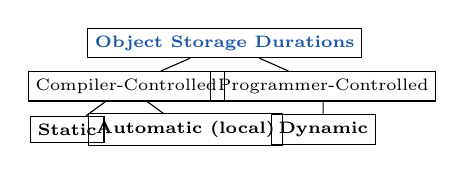
\begin{tikzpicture}[level distance=0.55cm,
  level 1/.style={sibling distance=2.5cm},
  level 2/.style={sibling distance=1.5cm},every node/.style={shape=rectangle,draw,align=center}]
  \node {\small \textcolor{headcolor}{\textbf{Object Storage Durations}}}
    child {node {\small Compiler-Controlled}
      child {node {\small \textbf{Static}}}
      child {node {\small \textbf{Automatic (local)}}}
    }
    child {node {\small Programmer-Controlled}
    child {node {\small \textbf{Dynamic}}}
    };
\end{tikzpicture}
%\end{figure}
\end{minipage}
\hspace{3pt}
\begin{minipage}{0.25 \textwidth}
    \small %Objects have \textit{lifetimes}, determined by storage duration, during which they're legal to use. 
    %Object lifetimes are determined by storage durations.
    %\smallskip
    Static objects "live" for essentially a program's runtime. Local objects' lifetimes are tied to scope (e.g. a block of code or pair of curly braces). Dynamic objects are manually created/destroyed.
    %\smallskip
    % \begin{itemize}[leftmargin=*,align=parleft]
    % \setlength\itemsep{0pt}
    %     \item Static: lifetime is essentially a program's runtime.
    %     \item Local: lifetime tied to scope (e.g. a block of code).
    %     \item Dynamic: must be explicitly created/destroyed.
    % \end{itemize}
    \smallskip
    \begin{itemize}[leftmargin=*,align=parleft]
    \setlength\itemsep{0pt}
    \item[\textcolor{info}{{\faInfoCircle}}] Objects declared in a loop body (between the \code{\{\}}) are created/destroyed each time the loop repeats.
\end{itemize}
    
    %Static = lifetime is essentially a program's entire runtime. Local = lifetime tied to scope (e.g. a block of code/pair of {\lstinline |{}|}). Dynamic = must be explicitly created/destroyed.
\end{minipage}


% \begin{itemize}[leftmargin=*,align=parleft]
%     \setlength\itemsep{0pt}
%     \item[\textcolor{info}{{\faInfoCircle}}] Objects created in a loop body (between the \myinline{\{\}}) are created/destroyed each time the loop repeats.
% \end{itemize}

%\myinline{new} \textbf{and} \myinline{delete} \textbf{operators}: used to allocate/deallocate large objects to dynamic (heap) memory. Note that the \myinline{new} keyword evaluates to a pointer (example syntax: \myinline{Matrix *m_ptr = new Matrix;})
% \begin{itemize}[leftmargin=*,align=parleft]
%     \setlength\itemsep{0pt}
%     \item[\textcolor{info}{{\faInfoCircle}}] Local objects are destroyed in the opposite order that they were created in.
% \end{itemize}
\smallskip

\textbf{Atomic (primitive) types}: objects that can't be subdivided into smaller objects; includes \code{int}, \code{double}, \code{bool}, \code{float}, \code{char}, and all pointer types. Atomic objects are default-initialized to undefined values. 

% \begin{itemize}[leftmargin=*,align=parleft]
%     \setlength\itemsep{0pt}
%     \item[\textcolor{info}{{\faInfoCircle}}] Division of integral types ignores remainders. E.g. \myinline{(5 / 2) == 2} and \myinline{(13 / 3) == 3}.
% \end{itemize}
\smallskip

%\textbf{Casting}: converting a value of one data type to a value of another type in an operation. Examples of type casts are: integral (e.g. \myinline{int}) $\leftrightarrow$ floating point (e.g. \myinline{double}), or any built-in type $\rightarrow$ \myinline{bool}. C++ supports both \textit{explicit} and \textit{implicit} up and down-casts.

%\vspace{-2pt}

% \begin{tcbraster}[raster columns=2, sharp corners, raster after skip=3pt, raster before skip=0pt,
%                   raster equal height, raster column skip=-.5mm]

% \begin{tcolorbox}[top=-5pt,bottom=-5pt,left=-1pt,right=-1pt,center title,toptitle=-0.6mm,
%   bottomtitle=-0.6mm,boxrule=0.5pt,arc=0pt]
% {\lstset{literate=% Colors the digits
%    *{0}{{{\color{vscode_green!100!black}0}}}1
%     {1}{{{\color{vscode_green!100!black}1}}}1
%     {2}{{{\color{vscode_green!100!black}2}}}1
%     {3}{{{\color{vscode_green!100!black}3}}}1
%     {4}{{{\color{vscode_green!100!black}4}}}1
%     {5}{{{\color{vscode_green!100!black}5}}}1
%     {6}{{{\color{vscode_green!100!black}6}}}1
%     {7}{{{\color{vscode_green!100!black}7}}}1
%     {8}{{{\color{vscode_green!100!black}8}}}1
%     {9}{{{\color{vscode_green!100!black}9}}}1
%     %{<<}{{{\color{operator}<\/<}}}2
% }
%               \begin{lstlisting}[style = mystyle]
% // Four different ways to initialize an int to 5
% int a = 5; int b(5); int c{5}; int d = {5};
% \end{lstlisting}
% }
% \end{tcolorbox}
% \begin{tcolorbox}[top=-5pt,bottom=-5pt,left=-1pt,right=-1pt,center title,toptitle=-0.6mm,
%   bottomtitle=-0.6mm,boxrule=0.5pt,arc=0pt]
% {\lstset{literate=% Colors the digits
%    *{0}{{{\color{vscode_green!100!black}0}}}1
%     {1}{{{\color{vscode_green!100!black}1}}}1
%     {2}{{{\color{vscode_green!100!black}2}}}1
%     {3}{{{\color{vscode_green!100!black}3}}}1
%     {4}{{{\color{vscode_green!100!black}4}}}1
%     {5}{{{\color{vscode_green!100!black}5}}}1
%     {6}{{{\color{vscode_green!100!black}6}}}1
%     {7}{{{\color{vscode_green!100!black}7}}}1
%     {8}{{{\color{vscode_green!100!black}8}}}1
%     {9}{{{\color{vscode_green!100!black}9}}}1
%     %{<<}{{{\color{operator}<\/<}}}2
% }
%               \begin{lstlisting}[style = mystyle]
% // Explicitly cast an int 'd' to a double 'e'
% double e = static_cast<double>(d);
% \end{lstlisting}
% }
% \end{tcolorbox}
% \end{tcbraster}

%\vspace{-2pt}
% \begin{itemize}[leftmargin=*,align=parleft]
% \setlength\itemsep{0pt}
% \item[\textcolor{info}{{\faInfoCircle}}] The syntax for explicit \textit{type-casting} is: \myinline{int x = static_cast<int>(my_double);}
% \end{itemize}


%Objects in C++ are \textbf{statically-typed}. Although an object may evaluate to a different type in an expression, the type of an object itself cannot change (class objects obey this rule too).


%\textcolor{headcolor}{\textbf{Stack Frames and the Activation Record/Call Stack}}

%The memory allocated for function data in a program (parameters and local variables) are stored in \textbf{stack frames}, a.k.a. activation records. 

%Functions require varying amounts of memory at runtime to store their parameters and local variables (and less importantly, temp objects, return addresses, etc). 

An \textbf{lvalue} is an object at some address in memory; an \textbf{rvalue} is a \textit{value} with no meaningful address.

The memory allocated to store a function's parameters and local variables during runtime is called a \textbf{stack frame} or activation record. The memory frame for the most-recently called function is added to the "top" of the \textbf{function call stack} and is destroyed when the function returns ("Last In First Out" ordering).
\smallskip
%(the memory frame for the last-called function is added to the top of the stack and is always the first frame to be destroyed). \smallskip

%Objects have \textit{lifetimes} during which it is legal to use them. In other words, all objects are created and destroyed at some point. An object's lifetime is determined by its storage duration.


%How to identify storage duration:

%\textcolor{info}{{\faInfoCircle}} An object that has dynamic storage duration is not associated with a variable at all. \smallskip

%\smallskip
%\textcolor{headcolor}{\textbf{Reference/Value Semantics}}

%The statement {\lstinline |x = y|} changes the value of {\lstinline |x|} to a \textit{copy} of {\lstinline |y|}'s data (\textbf{value semantics}). The statement {\lstinline |int &x = y|} makes {x} and {y} refer to the same object—in other words, that statement aliases {\lstinline |x|} to {\lstinline |y|} (\textbf{reference semantics}). Ref semantics are \textit{only} supported during initialization.

%\smallskip
% \begin{tcolorbox}[boxrule=0pt,left=1mm,right=1mm,top=0.75mm,bottom=0.75mm,boxsep=0mm,colback=orange!70!black,frame empty,arc=0mm,fontupper=\large\sffamily\bfseries]
% \begin{center}
%     \small{\textcolor{white}{\textbf{Procedural Abstraction, Testing, and Program Design}}}
% \end{center}
% \end{tcolorbox}
%\smallskip
\textcolor{headcolor}{\textbf{Procedural Abstraction and Program Design}}

%\textbf{Abstraction}: the principle of separating what something does (interface) from how it works (implementation) in order to manage complexity and hide details (guarding against mistakes). 

\textbf{Procedural Abstraction} involves using functions to break down a complex procedure into sub-tasks and separate the interface of a procedure (what it does) from implementation (how it works).

\textbf{Interface examples}: declarations in \code{.h} files, valid/invalid inputs, RME statements, \textit{signature} (function name and parameter types), return type, and ADT representation invariants.

\textbf{Implementation examples}: definitions in \code{.cpp} files and code/comments inside function bodies.

%TODO: include diagram

%Stack frames are created when a function is invoked and destroyed (thus freeing up memory) as soon as a function returns. 

%So if the same function is called three times over a program's runtime, three stack frames in total will be created for that function over the the program's runtime.

%(so if the same function is called twice over a program's runtime, \textit{two} stack frames for that function are created over the program's runtime). 

%\textcolor{headcolor}{\textbf{Organizing Code}}
%\textcolor{headcolor}{\textbf{RMEs}}


%Abstraction is the principle of separating how something works from what it does. 
%\textbf{Procedural abstraction}: breaking a complex task down into subtasks.

%Abstractions should be substitutable (an interface should work regardless of implementation details) and 
% \vspace*{-\baselineskip}
% \smallskip

% \begin{table}[h]
% %\resizebox{\textwidth}{!}{%
%  \footnotesize
% \def\arraystretch{1.0}
% \begin{tabular}{ |Sc|Sc|Sc| }
% % \hline
%     \hline 
%     \cellcolor{gray!8} Interface (What) & \cellcolor{gray!8} Implementation (How) \\
%     %\textcolor{headcolor}{\textbf{Mod Identities}} \\
%     \hline 
%      Function declaration in {\lstinline |.h|} file &  Function definition in {\lstinline |.cpp|} file \\
%      \hline 
%      Valid/invalid input values for the function &  Code inside function's curly braces \\
%      \hline 
%      RME clause before function declaration in {\lstinline |.h|} file &  Clarifying comments inside function \\
%     %\hline
%     %$(ab) \equiv (a \Mod{m})(b \Mod{m}) \Mod{m}$\\
%     \hline
% \end{tabular}
% %}
% \end{table}
% \vspace*{-\baselineskip}

%\textbf{REQUIRES}: requirements for a function to work properly. The implementation should assume these are met (it's good to \myinline{assert} that the conditions are met, but don't implement "fixes" for RME violations).
%and ADT representation invariants.

% \begin{itemize}[leftmargin=*,align=parleft]
%     \setlength\itemsep{0pt}
%     \item[\textcolor{info}{{\faInfoCircle}}] It's good practice—though not strictly necessary—to \myinline{assert} that the REQUIRES clause conditions are met in the function implementation (need to \myinline{#include <cassert>} for this).
% \end{itemize}

% \textbf{MODIFIES}: lists the entities \textit{outside the function} that might be modified (side effects). Ex: pass-by-ref parameters, I/O streams (e.g. \myinline{cout}, \myinline{cin}, file streams), global variables, etc. 

% \textbf{EFFECTS}: describes what the function actually does (but not how it works), what it returns, etc.

%\textcolor{headcolor}{\textbf{Writing Good Unit Tests}}

%\textbf{Unit tests} test individual pieces of code (e.g., functions). \textbf{System tests} test entire codebases at once, while \textbf{regression tests} are sets of unit and system tests that run whenever code is updated.

%Don't write unit tests that the compiler would catch, that don't compile, that violate the RME conditions, that target "unrealistic" bugs, or that break an interface. Do write test cases for simple cases and edge cases, make test cases specific, and use relatively "small" test cases (except for large input edge tests).

%Includes details about what modifications (if any) are made, and what the return value (if any) means.

% \begin{minipage}[t]{4.5cm}
%     \footnotesize
%     \center{\underline{Good Tests}} \smallskip
%     \begin{itemize}[leftmargin=*,align=parleft]
%         \item[\textcolor{blue}{{\faThumbsUp}}] Checks a mix of general and special (edge/stress) cases.
%         \item[\textcolor{blue}{{\faThumbsUp}}] Prioritizes realistic bugs
%         \item[\textcolor{blue}{{\faThumbsUp}}] Correct implementation = guaranteed pass
%     \end{itemize}
% \end{minipage}
% %\hspace{0pt}
% \begin{minipage}[t]{4.5cm}
%     \footnotesize
%     \center{\underline{Bad Tests}} \smallskip
%     \begin{itemize}[leftmargin=*,align=parleft]
%         \item[\textcolor{blue}{{\faThumbsDown}}] Violates R, M, or E of RME clause
%         \item[\textcolor{blue}{{\faThumbsDown}}] Tests bugs that a compiler would catch
%         \item[\textcolor{blue}{{\faThumbsDown}}] Does not respect interface
%     \end{itemize}
% \end{minipage}

%\smallskip
\begin{tcolorbox}[boxrule=0pt,left=1mm,right=1mm,top=0.75mm,bottom=0.75mm,boxsep=0mm,colback=orange!75!black,frame empty,arc=0mm,fontupper=\large\sffamily\bfseries]
\begin{center}
    \small{\textcolor{white}{\textbf{Pointers, Arrays and References}}}
\end{center}
\end{tcolorbox}

%\textcolor{headcolor}{\textbf{Pointers and their Uses}}

A \textbf{pointer} is a type of object that stores another object's memory address as its value.
\begin{itemize}[leftmargin=*,align=parleft]
    \setlength\itemsep{0pt}
    \item[\textcolor{error}{\faExclamationCircle}] An \code{int*} pointer can \textit{only} point to an \code{int}; an \code{int**} pointer can \textit{only} point to an \code{int*}; and so on. (Trying to, for example, make an \code{int*} pointer point to a \code{double} will cause a compile error.)
    %\smallskip
\end{itemize}

% \vspace*{-\baselineskip}
% \begin{figure}[H]
\smallskip
\begin{minipage}[h]{4.5cm}
      \small \textbf{Dereferencing}: getting the object at an address. Note that the \code{*} operator is used both to declare pointers and to dereference them (and the \code{\&} operator is used both to get an object's address and to declare references).
      
      %To the right, \myinline{ptr} is dereferenced with the \myinline{*} operator on lines \myinline{3} and \myinline{5}.
      %(Note that the star on line {\lstinline |3|} is not being used to dereference anything, it's being used to declare a pointer.)

% \begin{itemize}[leftmargin=*,align=parleft]
%       \setlength\itemsep{0pt}
%     \item[\textcolor{info}{{\faInfoCircle}}] The \myinline{&} operator is used both to get an object's address and to create a reference.
% \end{itemize}

   \end{minipage}
   \hspace{0pt}
   \begin{minipage}[h]{5.7cm}
   \begin{tcolorbox}[top=-5pt,bottom=-5pt,left=-1pt,right=-1pt,boxrule=0.5pt,arc=0pt]
              {\lstset{
    escapeinside=@@,
    literate=% Colors the digits
   *{0}{{{\color{vscode_green!100!black}0}}}1
    {1}{{{\color{vscode_green!100!black}1}}}1
    {2}{{{\color{vscode_green!100!black}2}}}1
    {3}{{{\color{vscode_green!100!black}3}}}1
    {4}{{{\color{vscode_green!100!black}4}}}1
    {5}{{{\color{vscode_green!100!black}5}}}1
    {6}{{{\color{vscode_green!100!black}6}}}1
    {7}{{{\color{vscode_green!100!black}7}}}1
    {8}{{{\color{vscode_green!100!black}8}}}1
    {9}{{{\color{vscode_green!100!black}9}}}1
    %{<<}{{{\color{operator}<\/<}}}2
}
              \begin{lstlisting}[style = mystyle]
int x = 3; int y = 4;
int* @ptr1@ = &x; int* @ptr2@ = &y; 
int** @ptr1\_ptr@ = &@ptr1@;
@ptr2@ = @ptr1@; // copies x's address from ptr1 to ptr2
@ptr1@ = &y; // ptr1 now points at y
**@ptr1\_ptr@ = 6; // now y == 6
*@ptr2@ = 2; // ptr2 still points to x, so now x == 2

\end{lstlisting}
}
%cout << *ptr; // dereferences ptr/prints 3
   \end{tcolorbox}
    \end{minipage}
    %\smallskip
% \end{figure}

% \vspace*{-\baselineskip}
% \smallskip
% \vspace*{-\baselineskip}
%\begin{figure}[H]
%\smallskip

\begin{minipage}[h]{2.95cm}
      \small \begin{itemize}[leftmargin=*,align=parleft]
      \setlength\itemsep{0pt}
    \item[\textcolor{info}{{\faInfoCircle}}] Printing a non-\code{char} pointer prints an address. (\code{char} pointers get printed as C-strings.)
    
    \item[\textcolor{info}{{\faInfoCircle}}] A reference to a reference is really another reference for the "original" object.
    %\item[\textcolor{info}{{\faInfoCircle}}] The \myinline{&} operator is used both to get an object's address and to create a reference.
    %{\lstinline |cout << &y << endl;|} would print {\lstinline |0x2714|}, and {\lstinline |cout << &x << endl;|} would print {\lstinline |0x2710|}. (Also, {\lstinline |cout << y << endl;|} would print {\lstinline |0x2710|}, and if {\lstinline |cout << &*ptr << endl;|} were added to the end of the program, it would print {\lstinline |0x2714|}).
\end{itemize}
   \end{minipage}
   \hspace{0pt}
   \begin{minipage}[h]{5.25cm}
   \begin{tcolorbox}[top=-5pt,bottom=-5pt,left=-1pt,right=-1pt,boxrule=0.5pt,arc=0pt]
              {\lstset{literate=% Colors the digits
   *{0}{{{\color{vscode_green!100!black}0}}}1
    {1}{{{\color{vscode_green!100!black}1}}}1
    {2}{{{\color{vscode_green!100!black}2}}}1
    {3}{{{\color{vscode_green!100!black}3}}}1
    {4}{{{\color{vscode_green!100!black}4}}}1
    {5}{{{\color{vscode_green!100!black}5}}}1
    {6}{{{\color{vscode_green!100!black}6}}}1
    {7}{{{\color{vscode_green!100!black}7}}}1
    {8}{{{\color{vscode_green!100!black}8}}}1
    {9}{{{\color{vscode_green!100!black}9}}}1
    %{<<}{{{\color{operator}<\/<}}}2
}
              \begin{lstlisting}[style = mystyle]
int x = 5;
int* y = &x; // creates pointer to x
int* z = y; // creates another pointer to x
int* &b = z; // creates reference b to pointer z
cout << *b << endl; // Prints 5
cout << y << endl; // prints 0x2710
cout << &(*z) << endl; // equiv. to cout << &x
cout << *(&z) << endl; // equiv. to cout << z
\end{lstlisting}
}
%cout << &y << endl; // prints 0x2714
   \end{tcolorbox}
    \end{minipage}
   \begin{minipage}[h]{1.75cm}
       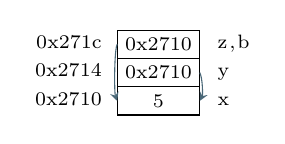
\begin{tikzpicture}[stack/.style={rectangle split, rectangle split parts=#1,draw, anchor=center}]
\node(s)[stack=3]  {
                 {\lstinline |0x2710|}    % text
\nodepart{two}   {\lstinline |0x2710|}     % two
\nodepart{three} {\lstinline |5|}      % three
};
% Adding comments and pointers
\node[anchor=mid west] at (s.one east){{\lstinline | z,b|}};
\node[anchor=mid west] at (s.two east){{\lstinline | y|}};
\node[anchor=mid west] at (s.three east){{\lstinline | x|}};
\node[anchor=mid east] at (s.one west){{\lstinline |0x271c |}};
\node[anchor=mid east] at (s.two west){{\lstinline |0x2714 |}};
\node[anchor=mid east] at (s.three west){{\lstinline |0x2710 |}};
\draw[cyan!40!black,->,>=stealth](s.two east) .. controls ($(s.two split)+(16pt,3pt)$) 
  and ($(s.two split)+(16pt,-3pt)$) .. (s.three east);
  \draw[cyan!40!black,->,>=stealth](s.one west) .. controls ($(s.one split)+(-16pt,3pt)$) 
  and ($(s.two split)+(-16pt,-2pt)$) .. (s.three west);

       \end{tikzpicture}
   \end{minipage}%
% \end{figure}
% \vspace*{-\baselineskip} 
% \smallskip

%\smallskip

% \begin{itemize}[leftmargin=*,align=parleft]
%     \item[\textcolor{warning}{{\faWarning}}] Watch out: the {\lstinline |&|} and {\lstinline |*|} symbols mean different things depending on context. 
% \end{itemize}

\smallskip
\textbf{Null pointer}: a pointer that holds address \code{0x0} (which no object can be located at) and implicitly converts to \code{false}. Any pointer can be nulled by setting it equal to \code{nullptr} (or \code{0}, or \code{NULL}).

% \begin{itemize}[leftmargin=*,align=parleft]
% \setlength\itemsep{0pt}
% \item[\textcolor{info}{{\faInfoCircle}}] The conditionals \myinline{if (ptr != nullptr)} and \myinline{if (ptr)} both evaluate to \myinline{true} for non-null pointers.
% \end{itemize}

% \begin{itemize}[leftmargin=*,align=parleft]
%     \item[\textcolor{info}{{\faInfoCircle}}] \textit{Any} pointer variable (regardless of type) can be set equal to {\lstinline |nullptr|}.
% \end{itemize}

\smallskip
\textcolor{headcolor}{\textbf{Common Pointer/Reference Errors}}
\begin{itemize}[leftmargin=*,align=parleft]
    \setlength\itemsep{0.0pt}
    %\item[\textcolor{warning}{{\faWarning}}] Uninitialized pointer variables do \textit{not} have a {\lstinline |nullptr|} value by default; \underline{like all atomic objects}, pointers that aren't explicitly initialized are default initialized to an undefined value, i.e. junk data.
    \item[\textcolor{warning}{{\faWarning}}] Dereferencing an uninitialized pointer results in undefined behavior, as (like all atomic objects) pointers that aren't explicitly initialized are default-initialized to an undefined value (\textit{not} \code{nullptr}).
    \vspace{0pt}
    %(the program may or may not crash, the pointer may take on a random value, etc).
    
    \item[\textcolor{warning}{{\faWarning}}] Dereferencing a null pointer also leads to undefined behavior (almost always a program crash).
    \vspace{0pt}

     \item[\textcolor{error}{{\faExclamationCircle}}] An uninitialized reference or a reference-to-non-\code{const} that's bound to an rvalue won't compile.
    
     \item[\textcolor{warning}{{\faWarning}}] If a function returns a pointer or reference to one of its local variables (which die when the function returns), dereferencing that pointer or using that reference produces undefined behavior. 
     %Functions should only return pointers or references to objects whose lifetimes extend beyond the function call.
     %(functions should only return references/pointers to objects that will outlive the function call).
     %\item[\textcolor{warning}{{\faWarning}}] A function that returns a pointer or reference to a local variable (which dies when the function returns) is a common source of undefined behavior.
\end{itemize}

%\smallskip
\begin{tcbraster}[raster columns=2, sharp corners, raster before skip=3pt, raster after skip=3pt,
                  raster equal height, raster column skip=-.5mm]
\begin{tcolorbox}[top=-5pt,bottom=-5pt,left=-1pt,right=-1pt,center title,toptitle=-0.6mm,
  bottomtitle=-0.6mm,boxrule=0.5pt,arc=0pt]
{\lstset{
escapeinside=@@,
literate=% Colors the digits
   *{0}{{{\color{vscode_green!100!black}0}}}1
    {1}{{{\color{vscode_green!100!black}1}}}1
    {2}{{{\color{vscode_green!100!black}2}}}1
    {3}{{{\color{vscode_green!100!black}3}}}1
    {4}{{{\color{vscode_green!100!black}4}}}1
    {5}{{{\color{vscode_green!100!black}5}}}1
    {6}{{{\color{vscode_green!100!black}6}}}1
    {7}{{{\color{vscode_green!100!black}7}}}1
    {8}{{{\color{vscode_green!100!black}8}}}1
    {9}{{{\color{vscode_green!100!black}9}}}1
    %{<<}{{{\color{operator}<\/<}}}2
}
              \begin{lstlisting}[style = mystyle]
int* danglingPtr(int x) { return &x; } // BUG
\end{lstlisting}
}
\end{tcolorbox}
\begin{tcolorbox}[top=-5pt,bottom=-5pt,left=-1pt,right=-1pt,center title,toptitle=-0.6mm,
  bottomtitle=-0.6mm,boxrule=0.5pt,arc=0pt]
{\lstset{
escapeinside=@@,
literate=% Colors the digits
   *{0}{{{\color{vscode_green!100!black}0}}}1
    {1}{{{\color{vscode_green!100!black}1}}}1
    {2}{{{\color{vscode_green!100!black}2}}}1
    {3}{{{\color{vscode_green!100!black}3}}}1
    {4}{{{\color{vscode_green!100!black}4}}}1
    {5}{{{\color{vscode_green!100!black}5}}}1
    {6}{{{\color{vscode_green!100!black}6}}}1
    {7}{{{\color{vscode_green!100!black}7}}}1
    {8}{{{\color{vscode_green!100!black}8}}}1
    {9}{{{\color{vscode_green!100!black}9}}}1
    %{<<}{{{\color{operator}<\/<}}}2
}
              \begin{lstlisting}[style = mystyle]
int& danglingRef(int x) { return x; } // BUG
\end{lstlisting}
}
\end{tcolorbox}
% \begin{tcolorbox}[top=-5pt,bottom=-5pt,left=-1pt,right=-1pt,center title,toptitle=-0.6mm,
%   bottomtitle=-0.6mm,boxrule=0.5pt,arc=0pt]
% {\lstset{
% escapeinside=@@,
% literate=% Colors the digits
%    *{0}{{{\color{vscode_green!100!black}0}}}1
%     {1}{{{\color{vscode_green!100!black}1}}}1
%     {2}{{{\color{vscode_green!100!black}2}}}1
%     {3}{{{\color{vscode_green!100!black}3}}}1
%     {4}{{{\color{vscode_green!100!black}4}}}1
%     {5}{{{\color{vscode_green!100!black}5}}}1
%     {6}{{{\color{vscode_green!100!black}6}}}1
%     {7}{{{\color{vscode_green!100!black}7}}}1
%     {8}{{{\color{vscode_green!100!black}8}}}1
%     {9}{{{\color{vscode_green!100!black}9}}}1
%     %{<<}{{{\color{operator}<\/<}}}2
% }
%               \begin{lstlisting}[style = mystyle]
% int* returnPtr(int &x ) 
%   { return &x; } // Ok
% \end{lstlisting}
% }
% \end{tcolorbox}
\end{tcbraster}

% \begin{itemize}[leftmargin=*,align=parleft]
%     \setlength\itemsep{0pt}
%     \item[\textcolor{error}{{\faExclamationCircle}}] All references must be explicitly initialized, and only references to \myinline{const} can bind to "literal" values.
% \end{itemize}

% \begin{minipage}[c]{0.45 \linewidth}
%    \begin{tcolorbox}[top=-5pt,bottom=-5pt,left=-1pt,right=-1pt,boxrule=0.5pt,arc=0pt,center title,toptitle=-0.6mm,
%   bottomtitle=-0.6mm,boxrule=0.5pt,arc=0pt,adjusted title={\footnotesize {\faThumbsDown } Dangling Pointer Bug},fonttitle=\large\sffamily\bfseries]
%               {\lstset{literate=% Colors the digits
%    *{0}{{{\color{vscode_green!100!black}0}}}1
%     {1}{{{\color{vscode_green!100!black}1}}}1
%     {2}{{{\color{vscode_green!100!black}2}}}1
%     {3}{{{\color{vscode_green!100!black}3}}}1
%     {4}{{{\color{vscode_green!100!black}4}}}1
%     {5}{{{\color{vscode_green!100!black}5}}}1
%     {6}{{{\color{vscode_green!100!black}6}}}1
%     {7}{{{\color{vscode_green!100!black}7}}}1
%     {8}{{{\color{vscode_green!100!black}8}}}1
%     {9}{{{\color{vscode_green!100!black}9}}}1
%     %{<<}{{{\color{operator}<\/<}}}2
% }
%               \begin{lstlisting}[style = mystyle]
% int* get_address(int x) { return &x; }
% // oops, x is a local object!

% void print(int val) {cout << val << endl;}

% int main() {
%   int a = 3;
%   int *dangling_ptr = get_address(a);
% } // value of dangling_ptr is undefined
% \end{lstlisting}
% }
%    \end{tcolorbox}
%     \end{minipage}
%     \hspace{0pt}
%    \begin{minipage}[c]{0.53 \linewidth}
%    \centering
%    \small
%        \begin{itemize}[leftmargin=*,align=parleft]
%                \item[\textcolor{warning}{{\faWarning}}] A pointer can outlive the object it points at. Here, \myinline{dangling_ptr} is initialized to the address of the local variable \myinline{x}, which is destroyed when  \myinline{get_address} returns (resulting in undefined behavior.) \smallskip
%                %so {\lstinline |*ptr|} ends up pointing to a dead object, causing undefined behavior.
               
%                THE FIX: pass \myinline{get_address}'s parameter by reference instead of by value—i.e., change the parameter to \myinline{get_address(int\& x)}. This would alias \myinline{x} to \myinline{a} in \myinline{main} (which doesn't "die" when \myinline{get_address} returns).
%                %instead of creating a local variable \myinline{x}.
%                %so \myinline{get_address} would instead return the address of \myinline{a}. 
%                %(which doesn't go out of scope when {\lstinline |get_address|} returns).
% \end{itemize}
%    \end{minipage} \smallskip
   % \begin{minipage}[c]{0.35 \linewidth}
   %    \footnotesize Pictured to the left are a code block and its (stack) memory diagram. In the memory diagram, {\lstinline |x|} is a variable and an object of type int (note that objects != variables).
   % \end{minipage}
% \end{figure}

% \vspace*{-\baselineskip}

%References and pointers both enable working between stack frames (across scopes) and indirection. \smallskip
%A number swap function that uses pointers and its stack diagram are shown below.

% \vspace*{-\baselineskip}
% \begin{figure}[H]
%\smallskip
%\smallskip
\begin{minipage}[h]{6.1cm} \small
\textcolor{headcolor}{\textbf{Pointers vs References}}

References and pointers both enable working between stack
frames (scopes) and indirection. Some ways they’re different:

    \begin{itemize}[leftmargin=*,align=parleft]
    \setlength\itemsep{0pt}
    \vspace{1pt}
    \item References are simply aliases for existing objects, while pointers are distinct objects with distinct values.
    \item Pointers must be dereferenced to access the objects they point at, while references are used "as-is".
    \item You can change what a (non-\code{const}) pointer points to, but a reference's binding to an object can't be changed.
    %\item A pointer is an object itself, a reference is simply a name/alias for an existing object.
    %(so reference semantics are only supported at initialization).
    %\item Pointers often take on null or undefined values, but references typically don't during normal programming.

    %references \textit{must} be explicitly initialized upon declaration, unlike pointers. Pointers must be dereferenced to access the objects they point at (references are used "as-is"). You can change the object that a pointer points to, while a reference's binding to an object cannot be changed (which also means a reference will always have the same value as the object it's aliased to). Lastly, pointers can be null or undefined, while constructing invalid/null references isn't something that normally happens.
\end{itemize}
        %Pointers can be null or undefined, while constructing invalid/null references isn't something that typically happens.

   % \centering\includegraphics[width=\linewidth]{fig67.png}
    \end{minipage}
    \hspace{0pt}
    \begin{minipage}[h]{4.1cm}
   \begin{tcolorbox}[top=-5pt,bottom=-5pt,left=-1pt,right=-1pt,center title,toptitle=-0.6mm,
  bottomtitle=-0.6mm,boxrule=0.5pt,arc=0pt,adjusted title={\footnotesize Using Pointers in a Function},fonttitle=\large\sffamily\bfseries]
              {\lstset{literate=% Colors the digits
   *{0}{{{\color{vscode_green!100!black}0}}}1
    {1}{{{\color{vscode_green!100!black}1}}}1
    {2}{{{\color{vscode_green!100!black}2}}}1
    {3}{{{\color{vscode_green!100!black}3}}}1
    {4}{{{\color{vscode_green!100!black}4}}}1
    {5}{{{\color{vscode_green!100!black}5}}}1
    {6}{{{\color{vscode_green!100!black}6}}}1
    {7}{{{\color{vscode_green!100!black}7}}}1
    {8}{{{\color{vscode_green!100!black}8}}}1
    {9}{{{\color{vscode_green!100!black}9}}}1
    %{<<}{{{\color{operator}<\/<}}}2
}
\begin{lstlisting}[style = mystyle]
int computeRange(int arr[], int N) {
  int* end = (arr + N);
  int* min = arr; int *max = arr;
  while (arr != end) {
    if (*arr < *min) { min = arr; }
    if (*arr > *max) { max = arr; }
    ++arr;
  }
  return (*max - *min);
}
\end{lstlisting}
}
% void swap_nums(int *x, int *y) {
%   int tmp = *x;
%   *x = *y;
%   *y = tmp;
% }
   \end{tcolorbox}
    \end{minipage}
% \end{figure}

% \vspace*{-\baselineskip}

%They differ in a few ways: references \textit{must} be explicitly initialized upon declaration, unlike pointers. Pointers must be dereferenced to access the objects they point at (whereas references are used "as-is"). Pointers can be null or undefined, and you can change the object that a pointer points to. A reference's binding to an object cannot be changed (so a reference always has the same value as the object it's aliased to), and it's harder to accidentally construct a null reference.

%\begin{itemize}
    %\setlength\itemsep{0pt}
    % \item Reference variables \textit{must} be initialized upon declaration, pointers don't need to be.
    %\item The address value a pointer holds can be changed to a different address (making it point to a different object) after initialization. The association between a reference and its object cannot be broken (all you can do is change the value stored by the object). 
    %So the same pointer can be used to access different objects, whereas a reference can only ever refer to one object.
   % \item Pointers can be null or undefined, and you can change the object that a pointer points to. While it's also possible to make an invalid pointer, it's harder to do so by accident (e.g. the compiler won't let you initialize a null reference), and a reference's binding to an object can't be changed.
%\end{itemize}

%\textcolor{headcolor}{\textbf{Basic properties and syntax}}

%\textbf{Arrays}: fixed-size containers that store sequences of objects of the same type (and thus, same size) in contiguous memory. 

\smallskip
\textcolor{headcolor}{\textbf{Arrays and Pointer Arithmetic}}

\textbf{Arrays}: fixed-size containers that store objects of the same type (and same size) in contiguous memory.

%\vspace{-2pt}

\begin{tcbraster}[raster columns=13, sharp corners, raster after skip=3pt, raster before skip=3pt,
                  raster equal height, raster column skip=-.5mm]
\begin{tcolorbox}[top=-5pt,bottom=-5pt,left=-8pt,right=-1pt,center title,toptitle=-0.6mm,
  bottomtitle=-0.6mm,boxrule=0.5pt,arc=0pt,raster multicolumn=4]
{\lstset{
escapeinside=@@,
literate=% Colors the digits
   *{0}{{{\color{vscode_green!100!black}0}}}1
    {1}{{{\color{vscode_green!100!black}1}}}1
    {2}{{{\color{vscode_green!100!black}2}}}1
    {3}{{{\color{vscode_green!100!black}3}}}1
    {4}{{{\color{vscode_green!100!black}4}}}1
    {5}{{{\color{vscode_green!100!black}5}}}1
    {6}{{{\color{vscode_green!100!black}6}}}1
    {7}{{{\color{vscode_green!100!black}7}}}1
    {8}{{{\color{vscode_green!100!black}8}}}1
    {9}{{{\color{vscode_green!100!black}9}}}1
    %{<<}{{{\color{operator}<\/<}}}2
}
              \begin{lstlisting}[style = mystyle,numbers=none]
int A[3] = {1,2}; // {1,2,0}
int B[3] = {}; // {0,0,0}
int C[] = {1,2}; // size == 2
\end{lstlisting}
}
\end{tcolorbox}
\begin{tcolorbox}[top=-5pt,bottom=-5pt,left=-8pt,right=-1pt,center title,toptitle=-0.6mm,
  bottomtitle=-0.6mm,boxrule=0.5pt,arc=0pt,raster multicolumn=5]
{\lstset{
escapeinside=@@,
literate=% Colors the digits
   *{0}{{{\color{vscode_green!100!black}0}}}1
    {1}{{{\color{vscode_green!100!black}1}}}1
    {2}{{{\color{vscode_green!100!black}2}}}1
    {3}{{{\color{vscode_green!100!black}3}}}1
    {4}{{{\color{vscode_green!100!black}4}}}1
    {5}{{{\color{vscode_green!100!black}5}}}1
    {6}{{{\color{vscode_green!100!black}6}}}1
    {7}{{{\color{vscode_green!100!black}7}}}1
    {8}{{{\color{vscode_green!100!black}8}}}1
    {9}{{{\color{vscode_green!100!black}9}}}1
    %{<<}{{{\color{operator}<\/<}}}2
}
              \begin{lstlisting}[style = mystyle,numbers=none]
int D[][2] = {1,2,3}; // {{1,2},{3,0}}
int E[][3] = {1,2,3}; // {{1,2,3}}
int F[3]; // CAUTION: uninitialized!
\end{lstlisting}
}
\end{tcolorbox}
\begin{tcolorbox}[top=-5pt,bottom=-5pt,left=-8pt,right=-1pt,center title,toptitle=-0.6mm,
  bottomtitle=-0.6mm,boxrule=0.5pt,arc=0pt,raster multicolumn=4]
{\lstset{
escapeinside=@@,
literate=% Colors the digits
   *{0}{{{\color{vscode_green!100!black}0}}}1
    {1}{{{\color{vscode_green!100!black}1}}}1
    {2}{{{\color{vscode_green!100!black}2}}}1
    {3}{{{\color{vscode_green!100!black}3}}}1
    {4}{{{\color{vscode_green!100!black}4}}}1
    {5}{{{\color{vscode_green!100!black}5}}}1
    {6}{{{\color{vscode_green!100!black}6}}}1
    {7}{{{\color{vscode_green!100!black}7}}}1
    {8}{{{\color{vscode_green!100!black}8}}}1
    {9}{{{\color{vscode_green!100!black}9}}}1
    %{<<}{{{\color{operator}<\/<}}}2
}
              \begin{lstlisting}[style = mystyle,numbers=none]
int @\ul{G}@[]; // ERROR: unclear size
int H[2@\ul{][}@] = {1,2,3,4}; // Same
int @\ul{I}@[] = {}; // Same
\end{lstlisting}
}
\end{tcolorbox}
\end{tcbraster}
%\vspace{-2pt}

%An important property of arrays is that they do NOT have inherent values, so attempting to set one array equal to another will lead to a compile error.

% \textbf{Initializing arrays}: \myinline{int arr[3] = \{ 1, 2 \};} initializes \myinline{arr} to \myinline{\{ 1, 2, 0 \}}. Also, if you omit the left-most dimension of an array during declaration, the compiler infers it from the size of the initializer list.
% Elements left out of an array's initializer list get implicitly initialized (atomics are \textit{value-initialized} to \myinline{0}). Ex: \myinline{int arr[3] = \{ 1, 2 \};} initializes \myinline{arr} to \myinline{\{ 1, 2, 0 \}}. Also, if you omit the left-most dimension of an array during declaration, the compiler infers it from the size of the initializer list.

% \begin{itemize}[leftmargin=*,align=parleft]
% \setlength\itemsep{0pt}
% \item[\textcolor{info}{{\faInfoCircle}}] \myinline{int arr[4] = \{ 1, 2 \};} initializes \myinline{arr} to \myinline{\{ 1, 2, 0, 0 \}}. Also, \myinline{int arr[] = \{ 4, 5, 7 \};} creates an array that can hold at most \myinline{3} elements.
% %Elements left out of an array's initializer list get implicitly initialized (atomics are \textit{value-initialized} to \myinline{0}). Ex: \myinline{int arr[3] = \{ 1, 2 \};} initializes \myinline{arr} to \myinline{\{ 1, 2, 0 \}}. Also, if you omit the left-most dimension of an array during declaration, the compiler will infer it from the size of the initializer list.
% % \item[\textcolor{info}{{\faInfoCircle}}] If you omit the left-most dimension of an array during declaration, the compiler will infer it from the number of elements in the initializer list.
% \end{itemize}


% When an array's initializer list is smaller than the array's size (and >0), uninitialized elements are implicitly initialized (atomics are \textit{value-initialized} to \myinline{0}). Ex: \myinline{int arr[3] = \{ 1, 2 \};} initializes \myinline{arr} to \myinline{\{ 1, 2, 0 \}}. Also, you can omit the left-most dimension of an array during declaration.

% \begin{itemize}[leftmargin=*,align=parleft]
%     \item[\textcolor{info}{{\faInfoCircle}}] This is why the left-most dimension of an array can have its size omitted during declaration.
%     % the compiler will infer it based on the size of the initializer list.
%     %\item[\textcolor{info}{{\faInfoCircle}}] When an array is used as a function parameter, it is passed by reference by default(?), unlike other data types.
% \end{itemize}

%\textcolor{headcolor}{\textbf{Arrays and Pointers}}
%\smallskip
\textbf{Array decay}: using an array in a context where a value is required causes the compiler to convert the array into a pointer to its first element. Array decay is why it's necessary to pass an array's size separately from the array to a function (or to indicate the end of an array with a \textit{sentinel character} like C-strings do).

\begin{itemize}[leftmargin=*,align=parleft]
    \setlength\itemsep{0pt}
    \item[\textcolor{warning}{{\faWarning}}] Dereferencing a pointer that goes past the bounds of an array results in undefined behavior. But merely \textit{using} a pointer that goes just past the end of an array without dereferencing it is well-defined.
\end{itemize}

%\smallskip

    %\begin{itemize}[leftmargin=*,align=parleft]
    %\setlength\itemsep{0pt}
     %\item[\textcolor{error}{\faExclamationCircle}] Pointer comparisons and subtraction are prohibited if the pointers point to objects of different types.
    %\item[\textcolor{warning}{{\faWarning}}] Pointer arithmetic is mainly useful on pointers into the same array (since only elements of the same array are guaranteed to be in contiguous memory). Pointer comparisons are only well-defined on pointers into the same array or pointers constructed from arithmetic operations on one pointer.
    %\item[\textcolor{warning}{{\faWarning}}] Pointer arithmetic and comparisons should generally only be done with pointers into the same array (or that were formed from arithmetic operations on one pointer). %Pointer comparisons are only well-defined on pointers into the same array or that were constructed from arithmetic operations on one pointer.
    
    %\item[\textcolor{warning}{{\faWarning}}] Dereferencing a pointer that goes past the bounds of an array results in undefined behavior. (But merely \textit{using} a pointer that goes just past the end of an array without dereferencing it is well-defined.)
    %as only array elements are guaranteed to be stored in contiguous memory. Pointer comparisons are only well-defined on pointers to elements of the same array or pointers constructed from arithmetic operations on the same pointer. 
%\end{itemize}

% \begin{itemize}[leftmargin=*,align=parleft]
%     \item[\textcolor{warning}{{\faWarning}}] Dereferencing a pointer that goes past the bounds of an array results in undefined behavior. (But merely \textit{using} a pointer that goes just past the end of an array without dereferencing it is well-defined.)
%     %To keep track of where an array ends, either keep track of the length separately (with an integer size or by constructing a pointer that's just past the end of an array) or store a \textbf{sentinel value} at the end.
% \end{itemize}

%\textbf{Pointer arithmetic}: Adding an \myinline{int} to a pointer yields another pointer that's offset from the original. Adding/subtracting two pointers of the same type returns an \myinline{int} representing how many objects apart they are. Pointer arithmetic is in terms of number of elements, not bytes.
%A function that adds 5 to each element of an array is shown below.

% \begin{itemize}[leftmargin=*,align=parleft]
%     \setlength\itemsep{0pt}
%     \item[\textcolor{info}{{\faInfoCircle}}] Pointer subtraction can return a negative number depending on the order of subtraction.
% \end{itemize}

% \begin{itemize}[leftmargin=*,align=parleft]
%     \setlength\itemsep{0pt}
%     \item[\textcolor{info}{{\faInfoCircle}}] Accessing the {\lstinline |i|}th element of an array (where {\lstinline |i|} is an arbitrary index) is always $\Theta (1)$ time complexity.
% \end{itemize}

% \vspace*{-\baselineskip}
% \begin{figure}[H]
\begin{minipage}[h]{5.1cm}
\smallskip
   \begin{tcolorbox}[top=-5pt,bottom=-5pt,left=-1pt,right=-1pt,boxrule=0.5pt,arc=0pt]
              {\lstset{literate=% Colors the digits
   *{0}{{{\color{vscode_green!100!black}0}}}1
    {1}{{{\color{vscode_green!100!black}1}}}1
    {2}{{{\color{vscode_green!100!black}2}}}1
    {3}{{{\color{vscode_green!100!black}3}}}1
    {4}{{{\color{vscode_green!100!black}4}}}1
    {5}{{{\color{vscode_green!100!black}5}}}1
    {6}{{{\color{vscode_green!100!black}6}}}1
    {7}{{{\color{vscode_green!100!black}7}}}1
    {8}{{{\color{vscode_green!100!black}8}}}1
    {9}{{{\color{vscode_green!100!black}9}}}1
    %{<<}{{{\color{operator}<\/<}}}2
}
              \begin{lstlisting}[style = mystyle]
void reverseArray(int arr[], int size) {
  for (int i = 0; i < (size / 2); ++i) {
    int temp = arr[i]; // needed for swapping
    arr[i] = arr[(size - 1 - i)];
    arr[(size - 1 - i)] = temp;
  } // Note: arr[i] == *(arr + i) == i[arr]
}
\end{lstlisting}
}
   \end{tcolorbox}
    \end{minipage}
     \hspace{0pt}
   \begin{minipage}[h]{5.1cm} 
    \small 
    %To the left is an example function that adds 5 to every element of an array. 
    Passing an array by value passes a pointer to its first element by value, so functions with array parameters like this one actually have pointer parameters.
    %Also, \myinline{arr[i]}, \myinline{*(arr + i)}, and \myinline{i[arr]} are all equivalent.
    %\smallskip
    \begin{itemize}[leftmargin=*,align=parleft]  \small 
    \smallskip
    \setlength\itemsep{0pt}
    \item[\textcolor{info}{{\faInfoCircle}}] The number of elements in an array \code{arr} is equal to \code{(sizeof(arr) / sizeof(*arr))}.
    %In this example, \myinline{sizeof(arr)} alone would return 12, not 3. 
    %Note that \myinline{sizeof(arr)} doesn't cause \myinline{arr} to decay.
    %as \myinline{sizeof()} doesn't need to get the value of an object.
\end{itemize}
    \end{minipage}
% \end{figure}
% \vspace*{-\baselineskip}

%\textbf{Pointer arithmetic}: You can add/subtract an integer from/to a pointer to get another pointer that is offset from the original, or you can subtract two pointers (iff they're the same type) to get an integer representing how many objects apart they are. \underline{Pointer arithmetic is in terms of number of elements, not bytes.} 

% \vspace*{-\baselineskip} 
% \smallskip
% \begin{figure}[H]
\begin{minipage}[h]{2.1cm}
      \small \begin{itemize}[leftmargin=*,align=parleft]
      \setlength\itemsep{0pt}
    \item[\textcolor{info}{{\faInfoCircle}}] \code{cout <\/< \&arr[0]}, \code{cout <\/< arr}, and \code{cout <\/< \&arr} would all print \code{0x1008}.
\end{itemize}
   \end{minipage}
   \begin{minipage}[h]{4.9cm} %\smallskip
   \begin{tcolorbox}[top=-5pt,bottom=-5pt,left=-1pt,right=-1pt,boxrule=0.5pt,arc=0pt]
              {\lstset{literate=% Colors the digits
   *{0}{{{\color{vscode_green!100!black}0}}}1
    {1}{{{\color{vscode_green!100!black}1}}}1
    {2}{{{\color{vscode_green!100!black}2}}}1
    {3}{{{\color{vscode_green!100!black}3}}}1
    {4}{{{\color{vscode_green!100!black}4}}}1
    {5}{{{\color{vscode_green!100!black}5}}}1
    {6}{{{\color{vscode_green!100!black}6}}}1
    {7}{{{\color{vscode_green!100!black}7}}}1
    {8}{{{\color{vscode_green!100!black}8}}}1
    {9}{{{\color{vscode_green!100!black}9}}}1
    %{<<}{{{\color{operator}<\/<}}}2
}
\begin{lstlisting}[style = mystyle]
int foo = 7;
int& bar = foo; // value of bar is foo (7)
int* ptr = &foo;
int arr[3] = { 4, 5, 9 };
cout << arr << endl; // prints 0x1008 (decay)
cout << (arr + 2) << endl; // prints 0x1010
\end{lstlisting}
} %cout << (&foo + 1) << endl; // prints 0x1004
   \end{tcolorbox}
    \end{minipage}
   \begin{minipage}[h]{2.9cm}
       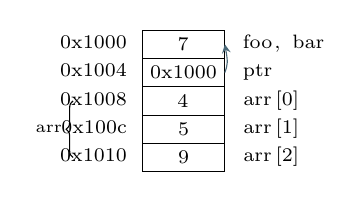
\begin{tikzpicture}[stack/.style={rectangle split, rectangle split parts=#1,draw, anchor=center}]
\node(s)[stack=5]  {
              {\lstinline |7|}    % one
\nodepart{two}                 {\lstinline |0x1000|}    % two
\nodepart{three}   {\lstinline |4|}     % three
\nodepart{four} {\lstinline |5|}      % four
\nodepart{five} {\lstinline |9|}      % five
};
% Adding comments and pointers
\node[anchor=mid west] at (s.one east){{\lstinline | foo, bar|}};
\node[anchor=mid west] at (s.two east){{\lstinline | ptr|}};
\node[anchor=mid west] at (s.three east){{\lstinline | arr[0]|}};
\node[anchor=mid west] at (s.four east){{\lstinline | arr[1]|}};
\node[anchor=mid west] at (s.five east){{\lstinline | arr[2]|}};
\node[anchor=mid east] at (s.one west){{\lstinline |0x1000 |}};
\node[anchor=mid east] at (s.two west){{\lstinline |0x1004 |}};
\node[anchor=mid east] at (s.three west){{\lstinline |0x1008 |}};
\node[anchor=mid east] at (s.four west){{\lstinline |0x100c |}};
\node[anchor=mid east] at (s.five west){{\lstinline |0x1010 |}};
%\draw[cyan!40!black,->,>=stealth](s.two east) .. controls ($(s.two split)+(16pt,3pt)$) 
  %and ($(s.two split)+(16pt,-3pt)$) .. (s.three east);
  %\draw[cyan!40!black,->,>=stealth](s.one west) .. controls ($(s.one split)+(-16pt,3pt)$) 
  %and ($(s.two split)+(-16pt,-2pt)$) .. (s.three west);
  \draw[black,decorate,decoration={brace,mirror,raise=25pt},thin] (s.three west) -- node[left,xshift= -26pt]{\footnotesize \lstinline |arr|} (s.five west);

    \draw[cyan!40!black,->,>=stealth](s.two east) .. controls ($(s.one split)+(16pt,-2pt)$) 
  and ($(s.two split)+(16pt,9pt)$) .. (s.one east);

       \end{tikzpicture}
   \end{minipage}
% \end{figure}
% \vspace*{-\baselineskip}

\smallskip
\begin{minipage}[h]{5.5cm}

\textbf{Pointer arithmetic}: adding an integer \code{n} to a pointer yields a pointer that is \code{n} \textit{objects} forward in memory. \smallskip

\textbf{Pointer subtraction}: Subtracting two pointers of the same type yields an integer (possibly a negative one) equal to the \textit{number of objects} between them. \smallskip

\textbf{Pointer comparison}: comparing pointers of the same type compares the addresses they store.

 % Adding an integer \myinline{n} to a pointer yields a pointer that's offset from the original by $n$ objects (not bytes). \smallskip
 
 % Subtracting two pointers of the same type yields an integer (not always a positive one) equal to the \textit{number of objects} of that type between them. \smallskip
 
 % Comparing pointers of the same type compares the addresses they store.
% \begin{itemize}[leftmargin=*,align=parleft]
%     \setlength\itemsep{0pt}
%     \item[\textcolor{info}{{\faInfoCircle}}] Pointer arithmetic is in terms of number of elements, not bytes.
% \end{itemize}
    \end{minipage}
    \hspace{0pt}
   \begin{minipage}[h]{4.7cm} 
      \begin{tcolorbox}[top=-5pt,bottom=-5pt,left=-1pt,right=-1pt,center title,toptitle=-0.6mm,
  bottomtitle=-0.6mm,boxrule=0.5pt,arc=0pt,adjusted title={\footnotesize Pointer Operations},fonttitle=\large\sffamily\bfseries]
              {\lstset{
    escapeinside=@@,
              literate=% Colors the digits
   *{0}{{{\color{vscode_green!100!black}0}}}1
    {1}{{{\color{vscode_green!100!black}1}}}1
    {2}{{{\color{vscode_green!100!black}2}}}1
    {3}{{{\color{vscode_green!100!black}3}}}1
    {4}{{{\color{vscode_green!100!black}4}}}1
    {5}{{{\color{vscode_green!100!black}5}}}1
    {6}{{{\color{vscode_green!100!black}6}}}1
    {7}{{{\color{vscode_green!100!black}7}}}1
    {8}{{{\color{vscode_green!100!black}8}}}1
    {9}{{{\color{vscode_green!100!black}9}}}1
    %{<<}{{{\color{operator}<\/<}}}2
}
              \begin{lstlisting}[style = mystyle]
// Mainly for pointers into the same array
double arr[4] = { 2.5, 5.0, 8.0, 7.0 };
double* ptr@1@ = &arr[0], *ptr@2@ = &arr[3];
cout << *arr << endl; // prints 2.5
cout << (ptr@2@ - ptr@1@) << endl; // prints 3
cout << (ptr@1@ - ptr@2@) << endl; // prints -3
(ptr@1@ > ptr@2@); // equates to false (0)
ptr@1@ += 2; // ptr1 now points at arr[2]
\end{lstlisting}
}
   \end{tcolorbox}
    \end{minipage}

    %\smallskip
    \begin{minipage}[h]{4.6cm} \small
    Using the \code{\&} operator on an array produces a pointer to the entire array, not a pointer to the first element or a pointer to a pointer (\code{\&} does not require a value, so it doesn't cause decay).
    %(as the \myinline{\&} operator doesn't require a value).
    %and arrays only decay when a value is required). \smallskip
    \end{minipage}
    \hspace{0pt}
    \begin{minipage}[h]{5.6cm} \small
   \begin{tcolorbox}[top=-5pt,bottom=-5pt,left=-1pt,right=-1pt,center title,toptitle=-0.6mm,
  bottomtitle=-0.6mm,boxrule=0.5pt,arc=0pt,
  %adjusted title={\footnotesize Creating/Using a Pointer to a Whole Array},fonttitle=\large\sffamily\bfseries
  ]
              {\lstset{literate=% Colors the digits
   *{0}{{{\color{vscode_green!100!black}0}}}1
    {1}{{{\color{vscode_green!100!black}1}}}1
    {2}{{{\color{vscode_green!100!black}2}}}1
    {3}{{{\color{vscode_green!100!black}3}}}1
    {4}{{{\color{vscode_green!100!black}4}}}1
    {5}{{{\color{vscode_green!100!black}5}}}1
    {6}{{{\color{vscode_green!100!black}6}}}1
    {7}{{{\color{vscode_green!100!black}7}}}1
    {8}{{{\color{vscode_green!100!black}8}}}1
    {9}{{{\color{vscode_green!100!black}9}}}1
    %{<<}{{{\color{operator}<\/<}}}2
}
              \begin{lstlisting}[style = mystyle]
int arr[4] = { 1, 2, 3, 4 };
int (*arr_ptr)[4] = &arr; // pointer to entire array
cout << (*arr_ptr)[2] << endl; // prints 3
// ++arr_ptr would increment by the size of 4 ints
\end{lstlisting}
}
   \end{tcolorbox}
   %\smallskip
\end{minipage}

\textbf{Traversal By Pointer}: arrays can be traversed by pointer (mostly used with C-strings and iterators).
\smallskip
%Traversal by index uses an {\lstinline |int|} index to access an array and modifies the index to traverse elements. Traversal by pointer involves "walking" a pointer across an array. \smallskip
% \begin{enumerate} 
%     \setlength\itemsep{0pt}
%     \item \textbf{By index}: use an {\lstinline |int|} index to access the array and modify the index to traverse through elements. This is the most common type of array traversal.
%     \item \textbf{By pointer}: "walk" a pointer across the elements of an array. These are applicable to traversing C-style strings and travel by iterator.
% \end{enumerate} \smallskip

% \vspace*{-\baselineskip} 
% \begin{figure}[H]
% \begin{minipage}[c]{3.6cm}
%    \begin{tcolorbox}[top=-5pt,bottom=-5pt,left=-1pt,right=-1pt,center title,toptitle=-0.6mm,
%   bottomtitle=-0.6mm,boxrule=0.5pt,arc=0pt,adjusted title={\footnotesize Traversal By Index},fonttitle=\large\sffamily\bfseries]
%               {\lstset{literate=% Colors the digits
%    *{0}{{{\color{vscode_green!100!black}0}}}1
%     {1}{{{\color{vscode_green!100!black}1}}}1
%     {2}{{{\color{vscode_green!100!black}2}}}1
%     {3}{{{\color{vscode_green!100!black}3}}}1
%     {4}{{{\color{vscode_green!100!black}4}}}1
%     {5}{{{\color{vscode_green!100!black}5}}}1
%     {6}{{{\color{vscode_green!100!black}6}}}1
%     {7}{{{\color{vscode_green!100!black}7}}}1
%     {8}{{{\color{vscode_green!100!black}8}}}1
%     {9}{{{\color{vscode_green!100!black}9}}}1
% }
%               \begin{lstlisting}[style = mystyle, language=C++]
% int const SIZE = 3;
% int arr[SIZE] = { -1, 7, 3 };

% for (int i = 0; i < SIZE; ++i) {
%   cout << arr[i] << endl;
% }

% \end{lstlisting}
% }
%    \end{tcolorbox}
%     \end{minipage}
   \begin{minipage}[h]{4.2cm} 
      \begin{tcolorbox}[top=-5pt,bottom=-5pt,left=-1pt,right=-1pt,center title,middle=-5pt,toptitle=-0.6mm,
  bottomtitle=-0.6mm,boxrule=0.5pt,arc=0pt,adjusted title={\footnotesize Traversal By Pointer: Pattern 1},fonttitle=\large\sffamily\bfseries]
              {\lstset{literate=% Colors the digits
   *{0}{{{\color{vscode_green!100!black}0}}}1
    {1}{{{\color{vscode_green!100!black}1}}}1
    {2}{{{\color{vscode_green!100!black}2}}}1
    {3}{{{\color{vscode_green!100!black}3}}}1
    {4}{{{\color{vscode_green!100!black}4}}}1
    {5}{{{\color{vscode_green!100!black}5}}}1
    {6}{{{\color{vscode_green!100!black}6}}}1
    {7}{{{\color{vscode_green!100!black}7}}}1
    {8}{{{\color{vscode_green!100!black}8}}}1
    {9}{{{\color{vscode_green!100!black}9}}}1
    %{<<}{{{\color{operator}<\/<}}}2
}
              \begin{lstlisting}[style = mystyle]
int const SIZE = 3;
int arr[SIZE] = {-1, 7, 2};
int *ptr = arr;
int *end = arr + SIZE; 
// int* end is "1-past-the-end" of arr
while (ptr < end) {
  cout << *ptr << endl;
  ++ptr; // "Walk" ptr across arr
} // Alternative to while loop below
\end{lstlisting}
}
\tcblower
\begin{lstlisting}[style = mystyle]
for (; ptr < end; ++ptr) { ... }
\end{lstlisting}
   \end{tcolorbox}
    \end{minipage}
    \hspace{0pt}
     \begin{minipage}[h]{6.0cm} 
      \begin{tcolorbox}[top=-5pt,bottom=-5pt,left=-1pt,right=-1pt,center title,toptitle=-0.6mm,
  bottomtitle=-0.6mm,boxrule=0.5pt,arc=0pt,adjusted title={\footnotesize Traversal by Pointer: Pattern 2 (C-String Sanitization)},fonttitle=\large\sffamily\bfseries]
              {\lstset{
    escapeinside=@@,
    literate=% Colors the digits
   *{0}{{{\color{vscode_green!100!black}0}}}1
    {1}{{{\color{vscode_green!100!black}1}}}1
    {2}{{{\color{vscode_green!100!black}2}}}1
    {3}{{{\color{vscode_green!100!black}3}}}1
    {4}{{{\color{vscode_green!100!black}4}}}1
    {5}{{{\color{vscode_green!100!black}5}}}1
    {6}{{{\color{vscode_green!100!black}6}}}1
    {7}{{{\color{vscode_green!100!black}7}}}1
    {8}{{{\color{vscode_green!100!black}8}}}1
    {9}{{{\color{vscode_green!100!black}9}}}1
    %{<<}{{{\color{operator}<\/<}}}2
}
              \begin{lstlisting}[style = mystyle]
void sanitizeUsername(Account *acc, char to_remove) {
  char* @ptr1@ = acc->username, *@ptr2@ = acc->username;
  while (*@ptr1@ && *@ptr2@) { // while not '\0'
    if (*@ptr2@ != to_remove) {
      *@ptr1@ = *@ptr2@;
      ++@ptr1@; // ++ptr1 only when a char gets copied
    }
    ++@ptr2@; // ++ptr2 every time the loop executes
  }
  *@ptr1@ = '\0'; // null-terminate string when done
} // NOTE: '\0' is the only char that evaluates to false
\end{lstlisting}
%      ++@ptr1@; // ++ptr1 only when a char gets copied
}
   \end{tcolorbox}
    \end{minipage}
% \end{figure}
% \vspace*{-\baselineskip} 

\begin{tcolorbox}[boxrule=0pt,left=1mm,right=1mm,top=0.75mm,bottom=0.75mm,boxsep=0mm,colback=darkyellow!85!black,frame empty,arc=0mm,fontupper=\large\sffamily\bfseries]
\begin{center}
    \small{\textcolor{white}{\textbf{The \myinlinewhite{const} Keyword}}}
\end{center}
\end{tcolorbox}

%\textcolor{headcolor}{\textbf{The Const Keyword}}
The \code{const} type qualifier stops objects from being modified after initialization. Note: \code{const} scalars must be explicitly-initialized to compile, and \code{const} class-type objects must have their data members initialized. %\smallskip

%The \myinline{const} type qualifier tells the compiler that an object's value shouldn't be changeable (attempting to modify a \myinline{const} object causes a compile error). \myinline{const} scalars must be explicitly-initialized to compile. \smallskip
%The syntax for declaring a simple type const is either {\lstinline |const int x = 3|} or {\lstinline |int const y = 4|}.
%\smallskip
\begin{minipage}[h]{5.3cm} \small
\textbf{\code{const} pointers}: pointers that can modify what they point at but cannot be re-pointed to different objects. 
\vspace{0.35ex}

\textbf{Pointer-to-\code{const}}: read-only pointers; pointers that can be re-bound but can't modify what they point at. 

\vspace{0.35ex}
\begin{itemize}[leftmargin=*,align=parleft] \setlength\itemsep{0pt}
    \item[\textcolor{error}{\faExclamationCircle}] A \code{const} pointer must be initialized to compile, but a pointer-to-\code{const} doesn't need to be.
\end{itemize} 
\vspace{0.35ex}

\textbf{Reference-to-\code{const}}: a read-only alias.

\vspace{0.35ex}
\textbf{\code{const} array}: an array of \code{const} elements. Note that the placement of \code{const} matters for arrays of pointers.
   \end{minipage}
   \hspace{0pt}
   \begin{minipage}[h]{4.9cm}
   \begin{tcolorbox}[center title,toptitle=-0.6mm,
bottomtitle=-0.6mm,top=-5pt,bottom=-5pt,middle=-5pt,left=-8pt,right=-1pt,boxrule=0.5pt,arc=0pt,adjusted title={\footnotesize Special \myinlinewhite{const} Type Syntax},fonttitle=\large\sffamily\bfseries
   %segmentation style={solid}
   ]
              {\lstset{literate=% Colors the digits
   *{0}{{{\color{vscode_green!100!black}0}}}1
    {1}{{{\color{vscode_green!100!black}1}}}1
    {2}{{{\color{vscode_green!100!black}2}}}1
    {3}{{{\color{vscode_green!100!black}3}}}1
    {4}{{{\color{vscode_green!100!black}4}}}1
    {5}{{{\color{vscode_green!100!black}5}}}1
    {6}{{{\color{vscode_green!100!black}6}}}1
    {7}{{{\color{vscode_green!100!black}7}}}1
    {8}{{{\color{vscode_green!100!black}8}}}1
    {9}{{{\color{vscode_green!100!black}9}}}1
    {const}{{{\color{blue} \textbf{const}}}}5
    %{<<}{{{\color{operator}<\/<}}}2
}
              \begin{lstlisting}[style = mystyle,numbers=none]
int x = 5;
int * const ptr_a = &x; // const pointer
const int * ptr_b = &x; // pointer-to-const
int const * ptr_c = &x; // pointer-to-const
const int * const ptr_d = &x; // both
int const * const ptr_e = &x; // both
\end{lstlisting}
}
\vspace{-4pt}
\tcbline
\vspace{-4pt}
{\lstset{literate=% Colors the digits
   *{0}{{{\color{vscode_green!100!black}0}}}1
    {1}{{{\color{vscode_green!100!black}1}}}1
    {2}{{{\color{vscode_green!100!black}2}}}1
    {3}{{{\color{vscode_green!100!black}3}}}1
    {4}{{{\color{vscode_green!100!black}4}}}1
    {5}{{{\color{vscode_green!100!black}5}}}1
    {6}{{{\color{vscode_green!100!black}6}}}1
    {7}{{{\color{vscode_green!100!black}7}}}1
    {8}{{{\color{vscode_green!100!black}8}}}1
    {9}{{{\color{vscode_green!100!black}9}}}1
    {const}{{{\color{blue} \textbf{const}}}}5
    %{<<}{{{\color{operator}<\/<}}}2
}
\begin{lstlisting}[style = mystyle,numbers=none]
const int &ref_a = x; // reference-to-const
int const &ref_b = 42; // reference-to-const
const int arr_a[2] = {1, 2}; // array of consts
int const arr_b[2] = {3, 4}; // array of consts
\end{lstlisting}
}
   \end{tcolorbox} 
    \end{minipage}

\begin{tcbraster}[raster columns=2, sharp corners, raster before skip=3pt, raster after skip=3pt,
                  raster equal height, raster column skip=-.5mm]
\begin{tcolorbox}[top=-5pt,bottom=-5pt,left=-8pt,right=-1pt,center title,toptitle=-0.6mm,
  bottomtitle=-0.6mm,boxrule=0.5pt,arc=0pt]
{\lstset{
escapeinside=@@,
literate=% Colors the digits
   *{0}{{{\color{vscode_green!100!black}0}}}1
    {1}{{{\color{vscode_green!100!black}1}}}1
    {2}{{{\color{vscode_green!100!black}2}}}1
    {3}{{{\color{vscode_green!100!black}3}}}1
    {4}{{{\color{vscode_green!100!black}4}}}1
    {5}{{{\color{vscode_green!100!black}5}}}1
    {6}{{{\color{vscode_green!100!black}6}}}1
    {7}{{{\color{vscode_green!100!black}7}}}1
    {8}{{{\color{vscode_green!100!black}8}}}1
    {9}{{{\color{vscode_green!100!black}9}}}1
    %{<<}{{{\color{operator}<\/<}}}2
}
              \begin{lstlisting}[style = mystyle, numbers=none]
const int* A[] = { ... }; // pointer-to-const array
\end{lstlisting}
}
\end{tcolorbox}
\begin{tcolorbox}[top=-5pt,bottom=-5pt,left=-8pt,right=-1pt,center title,toptitle=-0.6mm,
  bottomtitle=-0.6mm,boxrule=0.5pt,arc=0pt]
{\lstset{
escapeinside=@@,
literate=% Colors the digits
   *{0}{{{\color{vscode_green!100!black}0}}}1
    {1}{{{\color{vscode_green!100!black}1}}}1
    {2}{{{\color{vscode_green!100!black}2}}}1
    {3}{{{\color{vscode_green!100!black}3}}}1
    {4}{{{\color{vscode_green!100!black}4}}}1
    {5}{{{\color{vscode_green!100!black}5}}}1
    {6}{{{\color{vscode_green!100!black}6}}}1
    {7}{{{\color{vscode_green!100!black}7}}}1
    {8}{{{\color{vscode_green!100!black}8}}}1
    {9}{{{\color{vscode_green!100!black}9}}}1
    %{<<}{{{\color{operator}<\/<}}}2
}
              \begin{lstlisting}[style = mystyle,numbers=none]
int* const B[] = { ... }; // const pointer array
\end{lstlisting}
}
\end{tcolorbox}
\end{tcbraster}


% \textbf{const pointer}: a pointer that can't be re-bound to point at a different object (but can still be used to modify what it points at). Syntax: place the \myinline{const} keyword \underline{to the right} of a star, ex: \myinline{int * const ptr = &x;}.

% \textbf{Pointer-to-const}: a read-only pointer; a pointer that can't be used to modify whatever object it points to. Syntax: place the \myinline{const} keyword \underline{to the left} of a star, ex: \myinline{const int * ptr = &x;} or \myinline{int const * ptr = &x;}.

% \begin{itemize}[leftmargin=*,align=parleft]
%     \setlength\itemsep{0pt}
%     \item[\textcolor{info}{{\faInfoCircle}}] A pointer can be both a \myinline{const} pointer and a pointer-to-\myinline{const}. Ex: \myinline{const int* const ptr = \&x;}
% \end{itemize}

% \begin{itemize}[leftmargin=*,align=parleft]
%     \setlength\itemsep{0pt}
%     \item[\textcolor{info}{{\faInfoCircle}}] A pointer can be both a pointer-to-const and a const-pointer; they're not mutually exclusive.
% \end{itemize}

% \begin{itemize}[leftmargin=*,align=parleft]
%     \setlength\itemsep{0pt}
%     \item[\textcolor{info}{{\faInfoCircle}}] References, arrays, and functions are types that don't have values (and thus can't be declared as {\lstinline |const|} themselves).
% \end{itemize}

%\textbf{Reference-to-const}: essentially a read-only alias. Syntax: \myinline{const int &ref = x;} or \myinline{int const &ref = x;}.
%a reference itself cannot be {\lstinline |const|}, but a "reference-to-const" can be created, which is 

%\textbf{const Arrays}: an array whose elements cannot be modified after initialization (e.g. \myinline{const int arr[3]}).

%declaring an array as \myinline{const} (e.g. \myinline{const int arr[3]}) makes all of its elements \myinline{const}.

%\textbf{const Arrays}: \myinline{const double arr[3] = } \myinline{ { 1.1, 2.3, -4.5 }; } creates an array of three \myinline{const} doubles.

%an array can have {\lstinline |const|} elements. Ex: {\lstinline |const double arr[3] = {1.1, 2.3, -4.5};| } creates an array of three constant doubles. Note: {\lstinline |const|} can be placed to the left or right of the type. \smallskip

% Conversions between {\lstinline |const|} and non-{\lstinline |const|} elements must preserve the original const protections. This also means you can only pass a const variable to a function by reference-to-const or by pointer-to-const. \smallskip

% \vspace*{-\baselineskip} 
% \begin{figure}[H]

%\smallskip
\textcolor{headcolor}{\textbf{\myinlinewhite{const} Conversions and Passing}}

The compiler treats every pointer-to-\code{const} as if they point to a \code{const} object and every reference-to-\code{const} as if they're aliased to a \code{const} object. It won't allow conversions that could bypass existing \code{const} protections (so, e.g., you can assign a \code{const} pointer to a pointer-to-\code{const}, but the converse is \textit{not} true). %\smallskip

% \begin{itemize}[leftmargin=*,align=parleft]
%    \small  \setlength\itemsep{0pt}
%     \item[\textcolor{info}{{\faInfoCircle}}] The compiler assumes that every pointer-to-\myinline{const} is pointing at a \myinline{const} object (whether or not it's really true), and it won't allow conversions that could bypass the original \myinline{const} protections.
%     %\item[\textcolor{warning}{\faWarning}] A \myinline{const} instance of a \myinline{class} or \myinline{struct} cannot call non-\myinline{const} member functions.
%     %Conversions between \myinline{const} and non-\myinline{const} elements need to be \textit{at least as} restrictive as the original \myinline{const} protections. Also, the compiler assumes that every pointer-to-const is pointing to a \myinline{const} object (even if it's not the case). 
% \end{itemize}

%\smallskip
\begin{minipage}[c]{3.60cm}
%\small \textcolor{headcolor}{\textbf{\myinlinewhite{const} Conversions and Passing}}

%Conversions between \myinline{const} and non-\myinline{const} elements must preserve the original \myinline{const} protections, e.g. you can only pass a \myinline{const} variable to a function by reference/pointer-to-const (or by value).
%(You can pass a non-const int by const pointer/ref, though.)
   \begin{tcolorbox}[top=-5pt,bottom=-5pt,left=-1pt,right=-1pt,center title,toptitle=-0.6mm,
  bottomtitle=-0.6mm,boxrule=0.5pt,arc=0pt,
  %adjusted title={\footnotesize {\faThumbsDown } \myinlinewhite{const} Passing Errors},fonttitle=\large\sffamily\bfseries
  ]
{\lstset{
escapeinside=@@,
literate=% Colors the digits
   *{0}{{{\color{vscode_green!100!black}0}}}1
    {1}{{{\color{vscode_green!100!black}1}}}1
    {2}{{{\color{vscode_green!100!black}2}}}1
    {3}{{{\color{vscode_green!100!black}3}}}1
    {4}{{{\color{vscode_green!100!black}4}}}1
    {5}{{{\color{vscode_green!100!black}5}}}1
    {6}{{{\color{vscode_green!100!black}6}}}1
    {7}{{{\color{vscode_green!100!black}7}}}1
    {8}{{{\color{vscode_green!100!black}8}}}1
    {9}{{{\color{vscode_green!100!black}9}}}1
    %{<<}{{{\color{operator}<\/<}}}2
}
\begin{lstlisting}[style = mystyle]
void foo(string& a) {...}
void bar(string b) {...}
void func(const string& c) {...}
const string s = "Hello World";
bar(s); func(s); // both ok
foo(@\ul{s}@); foo(@\textcolor{clr-string}{\ul{"Hello"}}@); // ERRORS
\end{lstlisting}
}
   \end{tcolorbox}
\end{minipage}
%       \begin{tcolorbox}[top=-5pt,bottom=-5pt,left=-1pt,right=-1pt,center title,toptitle=-0.6mm,
%   bottomtitle=-0.6mm,boxrule=0.5pt,arc=0pt,adjusted title={\footnotesize {\faThumbsDown } Doesn't Compile},fonttitle=\large\sffamily\bfseries]
%               {\lstset{literate=% Colors the digits
%    *{0}{{{\color{vscode_green!100!black}0}}}1
%     {1}{{{\color{vscode_green!100!black}1}}}1
%     {2}{{{\color{vscode_green!100!black}2}}}1
%     {3}{{{\color{vscode_green!100!black}3}}}1
%     {4}{{{\color{vscode_green!100!black}4}}}1
%     {5}{{{\color{vscode_green!100!black}5}}}1
%     {6}{{{\color{vscode_green!100!black}6}}}1
%     {7}{{{\color{vscode_green!100!black}7}}}1
%     {8}{{{\color{vscode_green!100!black}8}}}1
%     {9}{{{\color{vscode_green!100!black}9}}}1
%     %{<<}{{{\color{operator}<\/<}}}2
% }
%               \begin{lstlisting}[style = mystyle]
% const int x = 3;
% int y = x; // Ok
% const int* cptr = &x; // Ok
% const int& cref = x; // Ok
% int* ptr = cptr; // Error 1
% int& ref = x; // Error 2
% \end{lstlisting}
% }
%    \end{tcolorbox}
\hspace{0pt}
\begin{minipage}[c]{6.60cm}
\begin{tcolorbox}[sidebyside,sidebyside gap=5pt,top=-5pt,bottom=-5pt,left=-1pt,right=-1pt,center title,toptitle=-0.6mm,
  bottomtitle=-0.6mm,boxrule=0.5pt,arc=0pt,
  %adjusted title={\footnotesize {\faThumbsDown } Invalid \myinlinewhite{const} Conversions},fonttitle=\large\sffamily\bfseries
  ]
              {\lstset{
              escapeinside=@@,
            literate=% Colors the digits
   *{0}{{{\color{vscode_green!100!black}0}}}1
    {1}{{{\color{vscode_green!100!black}1}}}1
    {2}{{{\color{vscode_green!100!black}2}}}1
    {3}{{{\color{vscode_green!100!black}3}}}1
    {4}{{{\color{vscode_green!100!black}4}}}1
    {5}{{{\color{vscode_green!100!black}5}}}1
    {6}{{{\color{vscode_green!100!black}6}}}1
    {7}{{{\color{vscode_green!100!black}7}}}1
    {8}{{{\color{vscode_green!100!black}8}}}1
    {9}{{{\color{vscode_green!100!black}9}}}1
    %{<<}{{{\color{operator}<\/<}}}2
}

              \begin{lstlisting}[style = mystyle]
const int x = 3;
int y = x; // Ok
const int* cptr = &x; // Ok
const int& cref = x; // Ok
int* ptr = @\ul{cptr}@; // ERROR 1
int& ref = @\ul{cref}@; // ERROR 2
  
\end{lstlisting}
}
\tcblower 
{\lstset{
escapeinside=@@,
literate=% Colors the digits
   *{0}{{{\color{vscode_green!100!black}0}}}1
    {1}{{{\color{vscode_green!100!black}1}}}1
    {2}{{{\color{vscode_green!100!black}2}}}1
    {3}{{{\color{vscode_green!100!black}3}}}1
    {4}{{{\color{vscode_green!100!black}4}}}1
    {5}{{{\color{vscode_green!100!black}5}}}1
    {6}{{{\color{vscode_green!100!black}6}}}1
    {7}{{{\color{vscode_green!100!black}7}}}1
    {8}{{{\color{vscode_green!100!black}8}}}1
    {9}{{{\color{vscode_green!100!black}9}}}1
    %{<<}{{{\color{operator}<\/<}}}2
}
\begin{lstlisting}[style = mystyle]
int x = 2, y = 5;
const int *x_ptr = &x;
int *y_ptr = &y;
*y_ptr = *x_ptr; // Ok
y_ptr @\ul{=}@ x_ptr; /* ERROR (even 
though x isn't const!) */
\end{lstlisting}
}
   \end{tcolorbox}
    \end{minipage}
%     \hspace{0pt}
%     \small \begin{minipage}[h]{2.9cm} \smallskip
%       \begin{tcolorbox}[top=-5pt,bottom=-5pt,left=-1pt,right=-1pt,center title,toptitle=-0.6mm,
%   bottomtitle=-0.6mm,boxrule=0.5pt,arc=0pt,adjusted title={\footnotesize {\faThumbsDown } Invalid Parameter},fonttitle=\large\sffamily\bfseries]
%               {\lstset{literate=% Colors the digits
%    *{0}{{{\color{vscode_green!100!black}0}}}1
%     {1}{{{\color{vscode_green!100!black}1}}}1
%     {2}{{{\color{vscode_green!100!black}2}}}1
%     {3}{{{\color{vscode_green!100!black}3}}}1
%     {4}{{{\color{vscode_green!100!black}4}}}1
%     {5}{{{\color{vscode_green!100!black}5}}}1
%     {6}{{{\color{vscode_green!100!black}6}}}1
%     {7}{{{\color{vscode_green!100!black}7}}}1
%     {8}{{{\color{vscode_green!100!black}8}}}1
%     {9}{{{\color{vscode_green!100!black}9}}}1
%     %{<<}{{{\color{operator}<\/<}}}2
% }
%               \begin{lstlisting}[style = mystyle]
% void my_func(int *a);
% // should be const int*a
% int main() {
%    const int x = 3;
%    my_func(&x); // error
% }
% \end{lstlisting}
% }
%    \end{tcolorbox}
%     \end{minipage}
% \end{figure}
% \vspace*{-\baselineskip} 

% \begin{itemize}[leftmargin=*,align=parleft]
%     \setlength\itemsep{0pt}
%     \item[\textcolor{info}{{\faInfoCircle}}] Pass objects by pointer or reference to make a function modify an object instead of creating and modifying a copy. If you don't need to change an object, pass by pointer-to-const or by reference-to-const to avoid accidental changes and to ensure const objects can be passed.
% \end{itemize}

%\smallskip
%If you need a function to modify an original object instead of a local copy, the only option is to pass it by reference or pointer-to-non-const. Otherwise, pass it by value (if the object is small, like an \myinline{int}) or by reference/pointer-to-\myinline{const} (if the object is large, like a string/vector/struct).

% \begin{itemize}[leftmargin=*,align=parleft]
%     \vspace{1pt}
%     \setlength\itemsep{-0.5pt}
%     \item \textbf{Pass by pointer/reference}: if you need to modify the original object (as opposed to a local copy).
%     \item \textbf{Pass by value}: if an object is small (e.g., an \myinline{int}) and you can't/don't need to modify the original.
%     \item \textbf{Pass by pointer/reference-to-\myinline{const}}: if you want to pass a large object without modifying it.
%     %\item \textbf{Pass by \myinline{const} pointer}: to stop a function from modifying the pointer itself (i.e., the address it stores).
%     %an object is large (e.g. vector/string/struct) and you don't need to modify it.
% \end{itemize}

\smallskip
$\bullet$ \textbf{Pass by pointer/reference}: if you need to modify the original object (as opposed to a local copy).

$\bullet$ \textbf{Pass by value}: if an object is small (e.g., an \code{int}) and you can't/don't need to modify the original.

$\bullet$ \textbf{Pass by pointer/reference-to-\code{const}}: if you want to pass a large object without modifying it.

% \tikzstyle{startstop} = [rectangle, rounded corners, minimum width=1.5cm, minimum height=0.5cm,text centered, draw=black, fill=red!30]
% \tikzstyle{process} = [rectangle, minimum width=1.5cm, minimum height=0.5cm, text centered, draw=black, fill=orange!30]
% \tikzstyle{decision} = [inner sep=-1.2ex, draw, diamond, aspect=1.75, minimum width=1.0cm, minimum height=0.4cm, text centered, draw=black, fill=green!30]
% \tikzstyle{arrow} = [thick,->,>=stealth]
% \begin{tikzpicture}[node distance=1cm]
% \node (start) [startstop] {Passing Semantics};
% \node (dec1) [decision, align=center, right of=start, xshift=1.5cm] {Need to \\ modify original \\ object?};
% \node (dec2) [decision, aspect=1.5, inner sep = 0.1ex, align=center, right of=dec1, xshift=1.5cm] {Object \\ size?};
% \node (pro2b) [process, align=center, right of=start, xshift=1.5cm, yshift=-1.2cm] {Pass by pointer or \\ reference-to-non-\myinline{const}};
% \draw [arrow] (start) -- (dec1);
% \draw [arrow] (dec1) -- node[anchor=base east] {Yes} (pro2b);
% \draw [arrow] (dec1) -- node[anchor=south] {No} (dec2);
% \end{tikzpicture}

%\textbf{Pass by pointer or reference if}: a function needs to modify the data of an original object.

%\textbf{Pass by pointer-to-const or reference-to-const if}: you need to pass a large object (vectors, strings, structs, etc) and you don't want to modify the original object's data.
%and/or you need to access but not alter the data of an object from a different scope.

%\textbf{Pass by value if}: an object is small (e.g. {\lstinline |int|}, {\lstinline |double|}, etc) and you only need a copy of the object.

% \begin{tcolorbox}[boxrule=0pt,left=1mm,right=1mm,top=0.75mm,bottom=0.75mm,boxsep=0mm,colback=cyan!50!black,frame empty,arc=0mm,fontupper=\large\sffamily\bfseries]
% \begin{center}
%     \small{\textcolor{white}{\textbf{Compound Objects and C-Style ADTs (structs)}}}
% \end{center}
% \end{tcolorbox}

% A \myinline{struct} is a class-type object composed of member subobjects (which, unlike C++ classes, are public by default). Unlike arrays, they have values, so you can copy the data of one \myinline{struct} to another via \myinline{=}. They are by default passed by value, so if you want a function to modify a \myinline{struct}, pass it by reference/pointer.

% \begin{itemize}[leftmargin=*,align=parleft]
% \setlength\itemsep{0pt}
% \item[\textcolor{info}{{\faInfoCircle}}] A \myinline{struct} or \myinline{class} instance can be declared as \myinline{const}, which prevents any of its data members from being modified. Like other \myinline{const}s, they must have their data members initialized.
% \end{itemize}

% \textbf{Dot} (\myinline{.}) \textbf{operator}: accesses the public member data of a \myinline{struct} (or \myinline{class}). Syntax: \myinline{className.elementName}.

% \textbf{Arrow} \myinline{->} \textbf{operator}: shorthand for \underline{pointer dereference followed by member access}. 

% %Ex: {\lstinline |Elevators->isServicing|} is equivalent to {\lstinline |(*Elevators).isServicing|}.
% %Use when accessing the member data of a struct or class that was passed by pointer. \smallskip 

% %\textcolor{headcolor}{\textbf{Abstract Data Types (ADTs)}}

% \textbf{Abstract Data Types (ADTs)}: a data type whose behavior and implementation are separated. ADTs are made up of both behaviors (functions) and heterogeneous data. \myinline{struct}s form the basis of C-style ADTs. \smallskip

% %Accessing the member data of an ADT object with the dot operator is said to "break" the interface. The \textit{behaviors} of an ADT should operate on an ADT struct instead. 

% If an ADT includes other ADTs, make sure to initialize member ADTs by calling their \myinline{init} functions or copying an existing object. It's also a good idea to use \myinline{assert} statements inside ADT member functions to check that \textbf{representation invariants}, conditions that all valid ADT instances must meet, are obeyed.

%ADTs separate the interface of a data type from its implementation (similar to how procedural abstraction separates a function's behavior from the way it works under-the-hood). {\lstinline |struct|}s form the basis of C-style ADTs.

% \vspace*{-\baselineskip}
% \begin{figure}[H]
% \begin{minipage}[h]{2.5cm}
%    \small 
%    Accessing the member data of an ADT object with the dot operator manually is said to "break" the interface. \smallskip 
   
%    The \textit{behaviors} of an ADT (implemented using pointer parameters) should operate on an ADT struct instead.
%     \end{minipage}
% \begin{minipage}[c]{5cm}
%    \begin{tcolorbox}[top=-5pt,bottom=-5pt,left=-1pt,right=-1pt,boxrule=0.5pt,arc=0pt]
%               {\lstset{literate=% Colors the digits
%    *{0}{{{\color{vscode_green!100!black}0}}}1
%     {1}{{{\color{vscode_green!100!black}1}}}1
%     {2}{{{\color{vscode_green!100!black}2}}}1
%     {3}{{{\color{vscode_green!100!black}3}}}1
%     {4}{{{\color{vscode_green!100!black}4}}}1
%     {5}{{{\color{vscode_green!100!black}5}}}1
%     {6}{{{\color{vscode_green!100!black}6}}}1
%     {7}{{{\color{vscode_green!100!black}7}}}1
%     {8}{{{\color{vscode_green!100!black}8}}}1
%     {9}{{{\color{vscode_green!100!black}9}}}1
% }
%               \begin{lstlisting}[style = mystyle, language=C++]
% struct Triangle { // triangle ADT
%   double a, b, c; // public by default
% }; // note the semicolon here!

% void Triangle_scale(Triangle *tri, double s) {
%   tri->a *= s; // s is the scaling factor
%   tri->b *= s;
%   tri->c *= s;
% }

% int main() {
%   Triangle t1 = { 3, 4, 5 };
%   Triangle_scale(&t1, 2); // sides = 6, 8, 10
% }

% \end{lstlisting}
% }
%    \end{tcolorbox}
%     \end{minipage}
%     \hspace{0pt}
%    \begin{minipage}[h]{2.2cm}
%    \smallskip
%    \centering\includegraphics[width=\linewidth]{07_triangle_scale.png}
%     \end{minipage}
% \end{figure}

% \vspace*{-\baselineskip}

% \begin{itemize}[leftmargin=*,align=parleft]
% \setlength\itemsep{0pt}
% \item[\textcolor{info}{{\faInfoCircle}}] It's a good idea to use \myinline{assert} statements inside ADT member functions to check that \textbf{representation invariants}, conditions that all valid ADT instances must meet, are obeyed.
% \end{itemize}

% \begin{itemize}[leftmargin=*,align=parleft]
%     \setlength\itemsep{0pt}
%     \item[\textcolor{warning}{{\faWarning}}] If an ADT includes other ADTs, make sure to initialize member ADTs by calling the member {\lstinline |init|} functions or copying a pre-existing object. 
%     %(e.g. in P2, the {\lstinline |Image_init|} function should also call the {\lstinline |Matrix_init|} function).
% \end{itemize}


\begin{tcolorbox}[boxrule=0pt,left=1mm,right=1mm,top=0.75mm,bottom=0.75mm,boxsep=0mm,colback=green!50!black,frame empty,arc=0mm,fontupper=\large\sffamily\bfseries]
\begin{center}
    \small{\textcolor{white}{\textbf{Strings, Streams and I/O}}}
\end{center}
\end{tcolorbox}

%\textbf{C-strings} are a built-in type (unlike \myinline{std::string}) represented by null-terminated \myinline{char} arrays. The \textbf{null char}, \myinline{\\0}, signals the end of a C-string by occupying its last index (necessary to avoid undefined behavior). 

%C-strings behave like arrays in most contexts, but output streams (e.g. \myinline{cout}) treat \myinline{char} arrays like strings.
%\begin{itemize}[leftmargin=*,align=parleft]
%\setlength\itemsep{0pt}
% \item[\textcolor{info}{{\faInfoCircle}}] The null character occupies the last index (taking up one space) in a C-string's array. 
%E.g. a {\lstinline |char|} array with 7 indices can hold strings containing up to 6 non-null characters. 
%\item[\textcolor{info}{{\faInfoCircle}}] The null char is the only \myinline{char} that evaluates to \myinline{false} (useful for writing traversal-by-pointer loops).
%(when traversing a C-string by pointer, you can take advantage of this—most programs that work with C-style strings use loops that execute until a pointer points to the null character.).
%\end{itemize}

%\textbf{Ways to Create and Use a C-string:}
% \begin{enumerate}
% \setlength\itemsep{0pt}
%     \item Create a pointer to a string literal: {\lstinline |const char *welcomeMsg = "Welcome to EECS 280!";|}
%     \item Create a (fixed-size) array to hold a copy of a C-string: {\lstinline |char hexColor[] = "00274C";|} (in this example, {\lstinline |hexColor|} can be modified, but it can only hold strings with \textit{six} non-null characters).
%     \item Create a large "buffer" string: {\lstinline |char filename[1024];|}
% \end{enumerate} 
% \smallskip
\textcolor{headcolor}{\textbf{Creating/Using C-Strings and Strings}}
 %\smallskip 
 
% \begin{itemize}[leftmargin=*,align=parleft]
% \setlength\itemsep{0pt}
% \item[\textcolor{info}{{\faInfoCircle}}] Output streams treat pointers to \myinline{char} arrays differently from pointers to other types of arrays.
% \end{itemize} \smallskip
    
   \begin{tcolorbox}[top=-5pt,bottom=-5pt,left=-1pt,right=-1pt,boxrule=0.5pt,arc=0pt,center title,toptitle=-0.6mm,
  bottomtitle=-0.6mm,boxrule=0.5pt,arc=0pt,before skip = 3pt, after skip = 3pt,
  %adjusted title={\footnotesize Ways to Create and Use a C-String},fonttitle=\large\sffamily\bfseries
  ]
              {\lstset{literate=% Colors the digits
   *{0}{{{\color{vscode_green!100!black}0}}}1
    {1}{{{\color{vscode_green!100!black}1}}}1
    {2}{{{\color{vscode_green!100!black}2}}}1
    {3}{{{\color{vscode_green!100!black}3}}}1
    {4}{{{\color{vscode_green!100!black}4}}}1
    {5}{{{\color{vscode_green!100!black}5}}}1
    {6}{{{\color{vscode_green!100!black}6}}}1
    {7}{{{\color{vscode_green!100!black}7}}}1
    {8}{{{\color{vscode_green!100!black}8}}}1
    {9}{{{\color{vscode_green!100!black}9}}}1
    %{<<}{{{\color{operator}<\/<}}}2
}
              \begin{lstlisting}[style = mystyle]
char color[] = "00274C"; // Create 7-element array (including \0) and copy a string literal to it
const char* cstr = "abcd"; // Only works for string literals; use .c_str() on string variables
cout << cstr << " " << *cstr << " " << &cstr[0] << endl; // prints "abcd a abcd" 
cout << (cstr + 1) << " " << *(cstr + 1) << " " << (*cstr + 1); // prints "bcd b 98" ('a' == 97)
string xyz = string(cstr); // Explicitly copy cstring to a string (implicit copy would work too)
\end{lstlisting}
}
%const char* new_cstr = xyz.c_str(); // Convert string to cstring via <string> function .c_str()
   \end{tcolorbox}
   %\smallskip

%    \begin{tcolorbox}[top=-5pt,bottom=-5pt,left=-1pt,right=-1pt,boxrule=0.5pt,arc=0pt,center title,toptitle=-0.6mm,
%   bottomtitle=-0.6mm,boxrule=0.5pt,arc=0pt,
%   %adjusted title={\footnotesize Ways to Create and Use a C-String},fonttitle=\large\sffamily\bfseries
%   ]
%               {\lstset{literate=% Colors the digits
%    *{0}{{{\color{vscode_green!100!black}0}}}1
%     {1}{{{\color{vscode_green!100!black}1}}}1
%     {2}{{{\color{vscode_green!100!black}2}}}1
%     {3}{{{\color{vscode_green!100!black}3}}}1
%     {4}{{{\color{vscode_green!100!black}4}}}1
%     {5}{{{\color{vscode_green!100!black}5}}}1
%     {6}{{{\color{vscode_green!100!black}6}}}1
%     {7}{{{\color{vscode_green!100!black}7}}}1
%     {8}{{{\color{vscode_green!100!black}8}}}1
%     {9}{{{\color{vscode_green!100!black}9}}}1
%     %{<<}{{{\color{operator}<\/<}}}2
% }
%               \begin{lstlisting}[style = mystyle]
% const char* msg = "Welcome!"; // Create CONST pointer to string literal (auto null-terminated)
% char color[] = "00274C"; // Create array to hold copy of a C-string (auto null-terminated)
% char cstr[5] = {'a','b','c','d','\0'}; // Create fixed-size char array (MANUALLY null-terminated)

% cout << cstr << " " << *(cstr) << " " << &cstr[0] << endl; // prints "abcd a abcd"
% cout << (cstr + 1) << " " << *(cstr + 1) << " " << (*cstr + 1); // prints "bcd b 98"

% cout << cstr << endl; // prints "abcd" (not an address). Note: cout << *(cstr) would print "a"
% cout << (cstr + 1) << endl; // prints "bcd"
% cout << *(cstr + 1) << endl; // prints "b"
% cout << (*cstr + 1) << endl; // prints "98" ('a' + 1). Note: A-Z == 65-90, a-z == 97-122
% string xyz = string(cstr); // Explicitly copy a cstring to a string (implicit call also works)
% const char* new_cstr = xyz.c_str(); // Convert string to cstring via <string> function .c_str()

% \end{lstlisting}
% }
%    \end{tcolorbox}

%C++ strings support the use of operators like {\lstinline |==, <, +, =|}, while 
%C-strings (being arrays) do not support the use of operators like {\lstinline |==, <, +, =|}. Also, C++ strings are default-initialized to empty strings of length 0.
%C-strings are mainly used when working with CL arguments.
%\textbf{C-String Library Functions (and Equivalent \myinline{std::string} Functions)}

%\vspace*{-\baselineskip}
%\begin{center}
\setlength\cellspacetoplimit{1pt}
\setlength\cellspacebottomlimit{1pt}
{\small \setlength{\tabcolsep}{0.6em}
    \resizebox{\linewidth}{!}{\begin{tabular}{*{6}{|Sc}|}
    \hhline{~|-|-|-|-|-|}
   \multicolumn{1}{Sc|}{} & \cellcolor{gray!13} Length & \cellcolor{gray!13} Copy Value & \cellcolor{gray!13} Index & \cellcolor{gray!13} Concatenate & \cellcolor{gray!13} Compare \\
    \hline
    {\textbf{\lstinline|<string>|}} \cellcolor{gray!13} & {\lstinline |str.length();|} & {\lstinline|str1 = str2;|} & {\lstinline|str[i];|} & {\lstinline|str1 += str2;|} & {\lstinline |str1 != str2;|} \\
    \hline
    {\textbf{\lstinline|<cstring>|}} \cellcolor{gray!13} & {\lstinline|strlen(cstr);| } & {\lstinline|strcpy(cstr1, cstr2);|} & {\lstinline|cstr[i];|} & {\lstinline|strcat(cstr1, cstr2);|} & {\lstinline |strcmp(cstr1, cstr2);|} \\
     \hhline{-|-|-|-|-|-|}
  %\hline
\end{tabular}}}
%\vspace*{-\baselineskip}

%{\footnotesize \textcolor{red}{*} \myinline{strcmp} returns \myinline{0} if the strings are identical;}
%\end{center}
%\vspace{-3pt}
%\vspace*{-\baselineskip}

%\smallskip

% \begin{tcolorbox}[boxrule=0pt,left=1mm,right=1mm,top=0.75mm,bottom=0.75mm,boxsep=0mm,colback=magenta!65!black,frame empty,arc=0mm,fontupper=\large\sffamily\bfseries]
% \begin{center}
%     \small{\textcolor{white}{\textbf{Streams and I/O}}}
% \end{center}
% \end{tcolorbox} 
\smallskip
\textcolor{headcolor}{\textbf{Streams and File I/O}} 
\smallskip

% \textbf{stdin redirection}: {\lstinline |./program.exe < file.txt|}

% \textbf{stdout redirection}: {\lstinline |./program.exe > file.txt|}

% \textbf{Pipeline} (send stdout from one program to stdin for another program): {\lstinline !./output.exe | input.exe !}


%\vspace*{-\baselineskip}

%\textcolor{headcolor}{\textbf{C.L.I. Commands}}
%\vspace*{-\baselineskip}
%\textcolor{headcolor}{\textbf{I/O Redirection }}
\setlength\cellspacetoplimit{1pt}
\setlength\cellspacebottomlimit{1pt}
{\small \setlength{\tabcolsep}{0.5em}
\resizebox{\linewidth}{!}{\begin{tabular}{|Sc|Sc|Sc|Sc|}
%\hline
% \multicolumn{3}{|Sc|}{{\textcolor{headcolor}{\textbf{C.L.I. Commands}}
%} \cellcolor{gray!8}} \\
\hline 
\myinline{stdin} Redirection \cellcolor{gray!13} & \myinline{stdout} Redirection \cellcolor{gray!13} & Pipeline \cellcolor{gray!13} & Combined Redirection \cellcolor{gray!13} \\ 
\hline 
{\lstinline |./main.exe < input.txt|} & {\lstinline |./main.exe > output.txt|} &{\lstinline !./output.exe | input.exe !} &{\lstinline |./main.exe < input.in > output.out|} \\ 
\hline
\end{tabular}} 
}

%\vspace*{-\baselineskip}
%{\footnotesize \textcolor{red}{*} If \myinline{output.txt} doesn't exist, this creates it (and then writes to it). If it does exist, this overwrites its contents.}

%\smallskip
% \begin{itemize}[leftmargin=*,align=parleft]
% \setlength\itemsep{0pt}
% \item[\textcolor{info}{{\faInfoCircle}}] Redirecting stdout to a non-existent file creates it; redirecting it to an existing file overwrites contents.
%\item[\textcolor{info}{{\faInfoCircle}}] stdin and stdout redirections can be "chained," ex: {\lstinline |./main.exe < main_test.in > main_test.out|}
%\end{itemize}

%\vspace*{-\baselineskip}

\smallskip

%To enable reading from/writing to files directly using {\lstinline |ifstream|} and {\lstinline |ofstream|} objects: add {\lstinline |#include <fstream>|} to the top of a program. 

% \vspace*{-\baselineskip}

% \begin{figure}[H]
    %\hspace{0pt}
    %\smallskip
   \begin{minipage}[h]{4.7cm} 
      \begin{tcolorbox}[top=-5pt,bottom=-5pt,left=-1pt,right=-1pt,center title,toptitle=-0.6mm,
  bottomtitle=-0.6mm,boxrule=0.5pt,arc=0pt,adjusted title={\footnotesize File I/O Ex 1: Print Lines From File},fonttitle=\large\sffamily\bfseries]
              {\lstset{
              escapeinside=@@,
              literate=% Colors the digits
   *{0}{{{\color{vscode_green!100!black}0}}}1
    {1}{{{\color{vscode_green!100!black}1}}}1
    {2}{{{\color{vscode_green!100!black}2}}}1
    {3}{{{\color{vscode_green!100!black}3}}}1
    {4}{{{\color{vscode_green!100!black}4}}}1
    {5}{{{\color{vscode_green!100!black}5}}}1
    {6}{{{\color{vscode_green!100!black}6}}}1
    {7}{{{\color{vscode_green!100!black}7}}}1
    {8}{{{\color{vscode_green!100!black}8}}}1
    {9}{{{\color{vscode_green!100!black}9}}}1
    %{<<}{{{\color{operator}<\/<}}}2
}
              \begin{lstlisting}[style = mystyle]
#include @\textcolor{delimit_red}{<}@@\textcolor{clr-string}{fstream}@@\textcolor{delimit_red}{>}@ // defines if/ofstreams
int main() {
  ifstream inFS; // or inFS("file.txt");
  inFS.open("file.txt");
  if (!inFS.is_open()) { return 1; }
  string str; // defaults to empty string
  while (getline(inFS, str)) {
    cout << str << endl;
  } // could close inFS via inFS.close();
} // inFS also closes when scope ends
\end{lstlisting}
}
   \end{tcolorbox}
    \end{minipage} 
    \hspace{0pt}
    \begin{minipage}[h]{5.5cm}
%\small \textcolor{headcolor}{\textbf{File I/O With Streams}}

\begin{tcolorbox}[top=-5pt,bottom=-5pt,left=-1pt,right=-1pt,center title,toptitle=-0.6mm,
  bottomtitle=-0.6mm,boxrule=0.5pt,arc=0pt,adjusted title={\footnotesize Ex 2: Copy One File's Contents to Another},fonttitle=\large\sffamily\bfseries]
              {\lstset{
              escapeinside=@@,
              literate=% Colors the digits
   *{0}{{{\color{vscode_green!100!black}0}}}1
    {1}{{{\color{vscode_green!100!black}1}}}1
    {2}{{{\color{vscode_green!100!black}2}}}1
    {3}{{{\color{vscode_green!100!black}3}}}1
    {4}{{{\color{vscode_green!100!black}4}}}1
    {5}{{{\color{vscode_green!100!black}5}}}1
    {6}{{{\color{vscode_green!100!black}6}}}1
    {7}{{{\color{vscode_green!100!black}7}}}1
    {8}{{{\color{vscode_green!100!black}8}}}1
    {9}{{{\color{vscode_green!100!black}9}}}1
    %{<<}{{{\color{operator}<\/<}}}2
}
              \begin{lstlisting}[style = mystyle]
#include @\textcolor{delimit_red}{<}@@\textcolor{clr-string}{fstream}@@\textcolor{delimit_red}{>}@
void copyFile(string infile, string outfile) {
  // fstreams can use C-strings as file names too
  ifstream inFS(infile);
  ofstream outFS(outfile);
  string @str@;
  while (inFS >> @str@) {
    outFS << @str@ << '\n';
  } // Note: >> and << stop at the first whitespace
} // Spaces and line breaks both act as separators
\end{lstlisting}
}
   \end{tcolorbox}

% \begin{itemize}[leftmargin=*,align=parleft]
% \setlength\itemsep{0pt}
% \item[\textcolor{info}{{\faInfoCircle}}] File streams close if they go out of scope or you call \myinline{.close()} on them.
% \end{itemize}

% \begin{itemize}[leftmargin=*,align=parleft]
% \setlength\itemsep{0pt}
%     \item[\textcolor{warning}{{\faWarning}}] Trying to read a stream into a non-matching object type makes the stream fail; to use it again, it must be cleared using \myinline{.clear()}.
%     %\item[\textcolor{warning}{{\faWarning}}] If using a \myinline{while} loop to read input from a file, make the "read" operation part of the loop condition.
%     %e.g. {\lstinline |while (inFS >> word)|}.
% \end{itemize}


% \begin{itemize}[leftmargin=*,align=parleft]
% \setlength\itemsep{0pt}
% \item[\textcolor{warning}{{\faWarning}}] \myinline{if/while(inFS)} implicitly converts \myinline{inFS} to \myinline{bool}, but \myinline{if/while(inFS == true)} does \textit{not} work without explicit casting.
% \end{itemize}

    \end{minipage} 
% \end{figure}
% \vspace*{-\baselineskip}

% \begin{itemize}[leftmargin=*,align=parleft]
%     \item[\textcolor{warning}{{\faWarning}}] When using a {\lstinline |while|} loop to read input from a file, the "read" operation should be part of the {\lstinline |while|} loop condition, e.g. {\lstinline |while (inFS >> word)|}.
% \end{itemize}
\smallskip

% \textbf{\myinline{istringstream}}: a stream that "simulates" input from a string. It and \myinline{ostringstream} are part of \myinline{<sstream>}.
%It (and \myinline{ostringstream}) are included in \myinline{<sstream>}. Syntax: \myinline{istringstream ss_input(string);}

%The syntax is the same as with \myinline{ifstream}, except any string is used instead of just a file name.

% \textbf{\myinline{ostringstream}}: a stream that captures output and stores it in a string (use \myinline{.str()} to get the string).

% \begin{itemize}[leftmargin=*,align=parleft]
% \setlength\itemsep{0pt}
% \item[\textcolor{info}{{\faInfoCircle}}] \myinline{ifstream}, \myinline{istringstream}, and \myinline{cin} can all be passed to a function with an \myinline{istream\&} parameter. Similarly, \myinline{ofstream}, \myinline{ostringstream}, and \myinline{cout} can all be passed to a function with an \myinline{ostream\&} parameter.
% \end{itemize} 
% \smallskip
%(can be used in place of an \myinline{ostream}). The \myinline{.str()} member function gets the string stored by an \myinline{ostringstream}.


%It and \myinline{istringstream} are part of the \myinline{<sstream>} library. The \myinline{.str()} member function gets the string stored by an \myinline{ostringstream}.
%, use the \myinline{.str()} member function.

%\vspace{-2pt}
% \begin{tcbraster}[raster columns=2, sharp corners, 
%                   raster equal height, raster column skip=-.5mm,
%                   raster after skip=0mm, raster before skip=0mm ]
% \begin{tcolorbox}[top=-5pt,bottom=-5pt,left=-1pt,right=-1pt,center title,toptitle=-0.6mm,
%   bottomtitle=-0.6mm,boxrule=0.5pt,arc=0pt]
% {\lstset{literate=% Colors the digits
%    *{0}{{{\color{vscode_green!100!black}0}}}1
%     {1}{{{\color{vscode_green!100!black}1}}}1
%     {2}{{{\color{vscode_green!100!black}2}}}1
%     {3}{{{\color{vscode_green!100!black}3}}}1
%     {4}{{{\color{vscode_green!100!black}4}}}1
%     {5}{{{\color{vscode_green!100!black}5}}}1
%     {6}{{{\color{vscode_green!100!black}6}}}1
%     {7}{{{\color{vscode_green!100!black}7}}}1
%     {8}{{{\color{vscode_green!100!black}8}}}1
%     {9}{{{\color{vscode_green!100!black}9}}}1
%     %{<<}{{{\color{operator}<\/<}}}2
% }
%               \begin{lstlisting}[style = mystyle]
% string input = "abc";
% istringstream inSS(input); // or inSS("abc")
% \end{lstlisting}
% }
% \end{tcolorbox}
% \begin{tcolorbox}[top=-5pt,bottom=-5pt,left=-1pt,right=-1pt,center title,toptitle=-0.6mm,
%   bottomtitle=-0.6mm,boxrule=0.5pt,arc=0pt]
% {\lstset{literate=% Colors the digits
%    *{0}{{{\color{vscode_green!100!black}0}}}1
%     {1}{{{\color{vscode_green!100!black}1}}}1
%     {2}{{{\color{vscode_green!100!black}2}}}1
%     {3}{{{\color{vscode_green!100!black}3}}}1
%     {4}{{{\color{vscode_green!100!black}4}}}1
%     {5}{{{\color{vscode_green!100!black}5}}}1
%     {6}{{{\color{vscode_green!100!black}6}}}1
%     {7}{{{\color{vscode_green!100!black}7}}}1
%     {8}{{{\color{vscode_green!100!black}8}}}1
%     {9}{{{\color{vscode_green!100!black}9}}}1
%     %{<<}{{{\color{operator}<\/<}}}2
% }
%               \begin{lstlisting}[style = mystyle]
% ostringstream outSS;
% Matrix_print(&mat, outSS); // Capture output
% \end{lstlisting}
% }
% \end{tcolorbox}
% \end{tcbraster}

% \smallskip
% \begin{itemize}[leftmargin=*,align=parleft]
% \setlength\itemsep{0pt}
% \item[\textcolor{info}{{\faInfoCircle}}] You can use an istringstream/ostringstream where an istream/ostream object is expected.
% \end{itemize}

% \begin{itemize}[leftmargin=*,align=parleft]
% \setlength\itemsep{0pt}
% \item[\textcolor{info}{{\faInfoCircle}}] istringstreams/ostringstreams are subtypes of istreams/ostreams, so you can pass an {\lstinline |istringstream|} where an {\lstinline |istream|} is expected (or an {\lstinline |ostringstream|} where an {\lstinline |ostream|} is expected).
% \end{itemize}


%\begin{itemize}[leftmargin=*,align=parleft]
   % \item[\textcolor{warning}{{\faWarning}}] If a read operation to an {\lstinline |ifstream|} object fails, the object retains its value from the last successful read. 
    % \item[\textcolor{warning}{{\faWarning}}] It's best to avoid mixing {\lstinline |getline()|} and regular insertion statements, because invisible {\lstinline |\n|} characters at the ends of lines can cause bugs. 
    % \item[\textcolor{warning}{{\faWarning}}] When setting up a {\lstinline |while|} loop to read input until the end of a file, the read operation should be the {\lstinline |while|} loop's condition (e.g. {\lstinline |while(inFS >> word)|})
%\end{itemize}

%\textcolor{headcolor}{\textbf{Mistakes to Avoid With File Input}}

% \vspace*{-\baselineskip} 
% \begin{figure}[H]
%    \begin{minipage}[h]{5.0cm} 
%       \begin{tcolorbox}[top=-5pt,bottom=-5pt,left=-1pt,right=-1pt,center title,toptitle=-0.6mm,
%   bottomtitle=-0.6mm,boxrule=0.5pt,arc=0pt,adjusted title={\footnotesize Separated Read/Check},fonttitle=\large\sffamily\bfseries]
%               {\lstset{literate=% Colors the digits
%    *{0}{{{\color{vscode_green!100!black}0}}}1
%     {1}{{{\color{vscode_green!100!black}1}}}1
%     {2}{{{\color{vscode_green!100!black}2}}}1
%     {3}{{{\color{vscode_green!100!black}3}}}1
%     {4}{{{\color{vscode_green!100!black}4}}}1
%     {5}{{{\color{vscode_green!100!black}5}}}1
%     {6}{{{\color{vscode_green!100!black}6}}}1
%     {7}{{{\color{vscode_green!100!black}7}}}1
%     {8}{{{\color{vscode_green!100!black}8}}}1
%     {9}{{{\color{vscode_green!100!black}9}}}1
% }
%               \begin{lstlisting}[style = mystyle, language=C++]
% ifstream inFS("hello.txt");

% while (inFS) { // Fix: while(inFS >> word) 
%    inFS >> word;
%    cout << word << endl;
%    // BUG: program prints the last word twice
% }
% \end{lstlisting}
% }
%    \end{tcolorbox}
%     \end{minipage}
%     \hspace{0pt}
%     \begin{minipage}[h]{5.0cm} 
%       \begin{tcolorbox}[top=-5pt,bottom=-5pt,left=-1pt,right=-1pt,center title,toptitle=-0.6mm,
%   bottomtitle=-0.6mm,boxrule=0.5pt,arc=0pt,adjusted title={\footnotesize Mixing {\lstinline |<<|} and getline},fonttitle=\large\sffamily\bfseries]
%               {\lstset{literate=% Colors the digits
%    *{0}{{{\color{vscode_green!100!black}0}}}1
%     {1}{{{\color{vscode_green!100!black}1}}}1
%     {2}{{{\color{vscode_green!100!black}2}}}1
%     {3}{{{\color{vscode_green!100!black}3}}}1
%     {4}{{{\color{vscode_green!100!black}4}}}1
%     {5}{{{\color{vscode_green!100!black}5}}}1
%     {6}{{{\color{vscode_green!100!black}6}}}1
%     {7}{{{\color{vscode_green!100!black}7}}}1
%     {8}{{{\color{vscode_green!100!black}8}}}1
%     {9}{{{\color{vscode_green!100!black}9}}}1
% }
%               \begin{lstlisting}[style = mystyle, language=C++]
% ifstream inFS("hello.txt");

% string word, line;
% inFS >> word;
% cout << word << endl;

% getline(inFS, line); // This gets a blank line
% cout << line << endl;

% \end{lstlisting}
% }
%    \end{tcolorbox}
%     \end{minipage}
% \end{figure}
% \vspace*{-\baselineskip} 

%\textcolor{headcolor}{\textbf{Streams and Functions}}

%Stream objects should be passed to functions by reference using generic istream/ostream types. Example: {\lstinline |void Image_print(const Image *img, std::ostream& os);|}

%\smallskip
\begin{minipage}[h]{5.0cm}
\textbf{\code{istringstream}}: an object that "simulates" \textit{input} with a string as its source. Note: an \code{istringstream}, an \code{ifstream} and \code{cin} can \textit{all} be passed to a function with a \code{std::istream\&} parameter. \smallskip

\textbf{\code{ostringstream}}: an object that captures \textit{output} and stores it in a string. Note: an \code{ostringstream}, an \code{ofstream} and \code{cout} can \textit{all} be passed to a function with a \code{std::ostream\&} parameter.
%(use \myinline{.str()} to get the string).

% \begin{itemize}[leftmargin=*,align=parleft]
% \setlength\itemsep{0pt}
% \item[\textcolor{info}{{\faInfoCircle}}] \myinline{ifstream}, \myinline{istringstream}, and \myinline{cin} can all be passed to a function with an \myinline{istream\&} parameter. Likewise, \myinline{ofstream}, \myinline{ostringstream}, and \myinline{cout} can all be passed to a function with an \myinline{ostream\&} parameter.
% \end{itemize} 
      
      %To the right, \myinline{ptr} is dereferenced with the \myinline{*} operator on lines \myinline{3} and \myinline{5}.
      %(Note that the star on line {\lstinline |3|} is not being used to dereference anything, it's being used to declare a pointer.)

% \begin{itemize}[leftmargin=*,align=parleft]
%       \setlength\itemsep{0pt}
%     \item[\textcolor{info}{{\faInfoCircle}}] The \myinline{&} operator is used both to get an object's address and to create a reference.
% \end{itemize}

   \end{minipage}
   \hspace{0pt}
   \begin{minipage}[c]{5.2cm}
   \begin{tcolorbox}[top=-5pt,bottom=-5pt,left=-1pt,right=-1pt,middle=-5pt,boxrule=0.5pt,arc=0pt]
              {
    \lstset{
    escapeinside=@@,
    literate=% Colors the digits
   *{0}{{{\color{vscode_green!100!black}0}}}1
    {1}{{{\color{vscode_green!100!black}1}}}1
    {2}{{{\color{vscode_green!100!black}2}}}1
    {3}{{{\color{vscode_green!100!black}3}}}1
    {4}{{{\color{vscode_green!100!black}4}}}1
    {5}{{{\color{vscode_green!100!black}5}}}1
    {6}{{{\color{vscode_green!100!black}6}}}1
    {7}{{{\color{vscode_green!100!black}7}}}1
    {8}{{{\color{vscode_green!100!black}8}}}1
    {9}{{{\color{vscode_green!100!black}9}}}1
    %{<<}{{{\color{operator}<\/<}}}2
}
              \begin{lstlisting}[style = mystyle]
#include @\textcolor{delimit_red}{<}@@\textcolor{clr-string}{sstream}@@\textcolor{delimit_red}{>}@ // defines stringstreams
void printPlusOne(istream& is, ostream& os) {
  int num = 0;
  while (is >> num) { os << (++num) << " "; }
} // Note: can't pass or return streams by value
...
istringstream inSS("1 3 5");
ostringstream outSS;
printPlusOne(inSS, outSS);
cout << outSS.str() << endl; // Prints "2 4 6"
\end{lstlisting}
}
   \end{tcolorbox}
    \end{minipage}
    %\smallskip

\smallskip
\textcolor{headcolor}{\textbf{Command-Line Arguments}}

%The arguments of a command (which come after the program name) are passed  to {\lstinline |main|}. 

\textbf{\code{argc}}: an \code{int} parameter of \code{main} representing the number of a command's arguments.

\textbf{\code{argv}}: an array of the arguments passed to a program. (Technically, \code{argv} is an array of pointers to the start of a C-strings—so \code{argv} is passed to \code{main} as a pointer to an array of pointers to C-strings).
%So \myinline{argv[0]} is a pointer to the start of a C-string that stores the name of the program.

% The \myinline{main} header in a program that accepts CLI arguments looks like: \myinline{int main(int argc, char *argv[])}
% \begin{itemize}
% \setlength\itemsep{0pt}
%     \item \myinline{argc}: an \myinline{int} parameter of \myinline{main} representing the number of arguments of a command.
%     \item \myinline{argv}: functionally, an array of the arguments (technically, \myinline{argv} is passed as a pointer to an array of pointers to C-strings of each argument.)
% \end{itemize}

% \begin{ubuntu}
% whoami `\StartConsole`
% root `\SU{root}` 
% hostname `\StartConsole`
% ubuntu`\SU{root}`
% ssh bob@remotehost`\StartConsole`
% _
% \end{ubuntu}

%\smallskip
\begin{minipage}[h]{6.3cm}
%\smallskip
  %  \begin{tcolorbox}[top=-5pt,bottom=-5pt,left=-1pt,right=-1pt,center title,toptitle=-0.6mm,
  % bottomtitle=-0.6mm,boxrule=0.5pt,arc=0pt,adjusted title={\footnotesize Number sum program with command-line arguments},fonttitle=\large\sffamily\bfseries]
  \begin{tcolorbox}[top=-5pt,bottom=-5pt,left=-1pt,right=-1pt,center title,toptitle=-0.6mm,
  bottomtitle=-0.6mm,boxrule=0.5pt,arc=0pt]
              {\lstset{
              escapeinside=@@,
              literate=% Colors the digits
   *{0}{{{\color{vscode_green!100!black}0}}}1
    {1}{{{\color{vscode_green!100!black}1}}}1
    {2}{{{\color{vscode_green!100!black}2}}}1
    {3}{{{\color{vscode_green!100!black}3}}}1
    {4}{{{\color{vscode_green!100!black}4}}}1
    {5}{{{\color{vscode_green!100!black}5}}}1
    {6}{{{\color{vscode_green!100!black}6}}}1
    {7}{{{\color{vscode_green!100!black}7}}}1
    {8}{{{\color{vscode_green!100!black}8}}}1
    {9}{{{\color{vscode_green!100!black}9}}}1
    %{<<}{{{\color{operator}<\/<}}}2
}
%#include @\textcolor{delimit_red}{<}@@\textcolor{clr-string}{iostream}@@\textcolor{delimit_red}{>}@
              \begin{lstlisting}[style = mystyle]
#include @\textcolor{delimit_red}{<}@@\textcolor{clr-string}{string}@@\textcolor{delimit_red}{>}@ // defines stoi()/stod()
int main(int argc, char* argv[]) { // char** argv also OK
  if (string(argv[1]) == "add") {
    int sum = 0;
    for (int i = 2; i < argc; i++) {
      sum += stoi(argv[i]);
    }
    cout << "Sum: " << sum << ", argc: " << argc << endl;
  } // pay attention to where the "actual" arguments start
} // Also remember to use stoi()/string() when needed

\end{lstlisting}
}
   \end{tcolorbox}
    \end{minipage}
    \hspace{0pt}
\begin{minipage}[h]{3.9cm} 
% \begin{ubuntu}
% ./main.exe add 7 2 `\StartConsole`
% Sum is: 9 `\SU{root}` `\StartConsole`
% argc is: 4 `\SU{root}` 
% ./main.exe add 1 2 3 `\StartConsole`
% Sum is: 6 `\SU{root}` `\StartConsole`
% argc is: 5 `\SU{root}` 
% _
% \end{ubuntu}
\begin{ubuntu}
./main.exe add 7 2 `\StartConsole`
Sum: 9, argc: 4 `\SU{root}`
./main.exe add 1 2 3 `\StartConsole`
Sum: 6, argc: 5 `\SU{root}`
_
\end{ubuntu}
\end{minipage}


% \begin{itemize}[leftmargin=*,align=parleft]
% \setlength\itemsep{0pt}
% \item[\textcolor{info}{{\faInfoCircle}}] \myinline{argv[0]} is the name of the program being executed, so the actual arguments start at \myinline{argv[1]}, and \myinline{argc} is 1 greater than the number of actual arguments. (Watch out for this when writing loops.)
% \end{itemize}

% \begin{itemize}[leftmargin=*,align=parleft]
%     \item[\textcolor{warning}{{\faWarning}}] If you have an \myinline{int} or \myinline{double} argument as (e.g.) the third argument, set an \myinline{int} equal to \myinline{stoi(argv[3])} or a \myinline{double} equal to \myinline{stod(argv[3])} to get the number (\myinline{stoi()}/\myinline{stod()} are part of \myinline{<string>}.)
%     \item[\textcolor{warning}{{\faWarning}}] To compare an element of \myinline{argv} to a string, you need to first wrap it in a \myinline{std::string()} 
%     %(you don't need to do this to assign a string the value of {\lstinline |argv[i]|}).
% \end{itemize}
 %\smallskip
% \begin{minipage}[h]{5.9cm} 
%       \begin{tcolorbox}[top=-5pt,bottom=-5pt,left=-1pt,right=-1pt,center title,toptitle=-0.6mm,
%   bottomtitle=-0.6mm,boxrule=0.5pt,arc=0pt,adjusted title={\footnotesize File I/O Ex 3: Add/subtract first N numbers in file},fonttitle=\large\sffamily\bfseries]
%               {\lstset{
%               escapeinside=@@,
%               literate=% Colors the digits
%    *{0}{{{\color{vscode_green!100!black}0}}}1
%     {1}{{{\color{vscode_green!100!black}1}}}1
%     {2}{{{\color{vscode_green!100!black}2}}}1
%     {3}{{{\color{vscode_green!100!black}3}}}1
%     {4}{{{\color{vscode_green!100!black}4}}}1
%     {5}{{{\color{vscode_green!100!black}5}}}1
%     {6}{{{\color{vscode_green!100!black}6}}}1
%     {7}{{{\color{vscode_green!100!black}7}}}1
%     {8}{{{\color{vscode_green!100!black}8}}}1
%     {9}{{{\color{vscode_green!100!black}9}}}1
%     %{<<}{{{\color{operator}<\/<}}}2
% }
%               \begin{lstlisting}[style = mystyle]
% int main(int argc, char* argv[]) {
%   ifstream inFS(argv[2]);
%   int N = stoi(argv[3]);
%   int total = 0, count = 0, num = 0;
%   while (inFS >> num && count != N) {
%     if (string(argv[1]) == "add") { total += num; }
%     else { total -= num; }
%     ++count;
%   }
%   cout << "total: " << total << endl;
% }
% \end{lstlisting}
% }
%    \end{tcolorbox}
%     \end{minipage} 
%     \hspace{0pt}
%     \begin{minipage}[h]{4.3cm}

% \begin{ubuntu}
% ./main.exe add num.txt 5 `\StartConsole`
% total: 15 `\SU{root}`
% ./main.exe sub num.txt 4 `\StartConsole`
% total: -10 `\SU{root}`
% _
% \end{ubuntu}
% \end{minipage} 

\begin{tcolorbox}[boxrule=0pt,left=1mm,right=1mm,top=0.75mm,bottom=0.75mm,boxsep=0mm,colback=cyan!60!darkgray,frame empty,arc=0mm,fontupper=\large\sffamily\bfseries]
\begin{center}
    \small{\textcolor{white}{\textbf{ADTs, Structs and Classes}}}
\end{center}
\end{tcolorbox}

\textcolor{headcolor}{\textbf{C-Style Structs and ADTs}}

A \code{struct} is a class-type object composed of member subobjects (heterogeneous data). They're passed by value by default, and they support assignment and initialization via the \code{=} operator. A \code{struct} or \code{class} object can also be declared as \code{const}, which prevents it and all of its data members from being modified.
%so if you want a function to modify a \myinline{struct} (as opposed to a local copy), pass it by reference/pointer.

\begin{itemize}[leftmargin=*,align=parleft]
\setlength\itemsep{0pt}
%\item[\textcolor{info}{{\faInfoCircle}}] Declaring a \myinline{struct} or \myinline{class} object as \myinline{const} prevents it and all of its data members from being modified (or assigned to via \myinline{=}) after initialization. They must have their data members initialized to compile.
%\item[\textcolor{info}{{\faInfoCircle}}] \myinline{const} class-type objects must have their data members initialized (or a runtime error will occur).

\item[\textcolor{error}{\faExclamationCircle}] You cannot call non-\code{const} member functions on a \code{const} instance of a \code{class} or \code{struct}. Also, you can't call non-\code{const} member functions from within a \code{const} member function.
\end{itemize}


%\textbf{Dot} (\myinline{.}) \textbf{operator}: accesses the public member data of a \myinline{struct} (or \myinline{class}). Syntax: \myinline{className.elementName;}

\textbf{Arrow} \code{->} \textbf{operator}: shorthand for a dereference followed by member access. \code{(*ptr).x == ptr->x;}

\begin{itemize}[leftmargin=*,align=parleft]
\setlength\itemsep{0pt}
\item[\textcolor{info}{{\faInfoCircle}}] Without parentheses, the dot and arrow operators have greater precedence than dereferencing.
%So \myinline{*(*foo_ptr).bar_ptr == *(foo_ptr->bar}, but \myinline{**foo_ptr.bar_ptr != *(foo_ptr->bar}.
\end{itemize}
%\begin{itemize}[leftmargin=*,align=parleft]
%\setlength\itemsep{0pt}
%\item[\textcolor{info}{\faInfoCircle}] Without parentheses, the dot/arrow operators have higher precedence than the dereference operator.
%\end{itemize}
% \vspace{-3pt}
% \begin{tcbraster}[raster columns=4, sharp corners, 
%                   raster equal height, raster column skip=-.5mm, raster after skip=0mm, raster before skip=0mm]
% \begin{tcolorbox}[top=-5pt,bottom=-5pt,left=-1pt,right=-1pt,center title,toptitle=-0.6mm,
%   bottomtitle=-0.6mm,boxrule=0.5pt,arc=0pt]
% {\lstset{literate=% Colors the digits
%    *{0}{{{\color{vscode_green!100!black}0}}}1
%     {1}{{{\color{vscode_green!100!black}1}}}1
%     {2}{{{\color{vscode_green!100!black}2}}}1
%     {3}{{{\color{vscode_green!100!black}3}}}1
%     {4}{{{\color{vscode_green!100!black}4}}}1
%     {5}{{{\color{vscode_green!100!black}5}}}1
%     {6}{{{\color{vscode_green!100!black}6}}}1
%     {7}{{{\color{vscode_green!100!black}7}}}1
%     {8}{{{\color{vscode_green!100!black}8}}}1
%     {9}{{{\color{vscode_green!100!black}9}}}1
%     %{<<}{{{\color{operator}<\/<}}}2
% }
%               \begin{lstlisting}[style = mystyle]
% struct Foo {
%   int bar = 5;
%   int* bar_ptr = &bar;
% };
% Foo foo;
% \end{lstlisting}
% }
% \end{tcolorbox}
% \begin{tcolorbox}[top=-5pt,bottom=-5pt,left=-1pt,right=-1pt,center title,toptitle=-0.6mm,
%   bottomtitle=-0.6mm,boxrule=0.5pt,arc=0pt, raster multicolumn=3]
% {\lstset{literate=% Colors the digits
%    *{0}{{{\color{vscode_green!100!black}0}}}1
%     {1}{{{\color{vscode_green!100!black}1}}}1
%     {2}{{{\color{vscode_green!100!black}2}}}1
%     {3}{{{\color{vscode_green!100!black}3}}}1
%     {4}{{{\color{vscode_green!100!black}4}}}1
%     {5}{{{\color{vscode_green!100!black}5}}}1
%     {6}{{{\color{vscode_green!100!black}6}}}1
%     {7}{{{\color{vscode_green!100!black}7}}}1
%     {8}{{{\color{vscode_green!100!black}8}}}1
%     {9}{{{\color{vscode_green!100!black}9}}}1
%     %{<<}{{{\color{operator}<\/<}}}2
% }
%               \begin{lstlisting}[style = mystyle]
% // Note: if no parentheses, dot and -> have precedence over dereference
% Foo* foo_ptr = &foo;
% cout << foo_ptr->bar << endl; // foo_ptr->bar equiv. to (*foo_ptr).bar
% cout << *(*foo_ptr).bar_ptr << endl;
% cout << *(foo_ptr->bar_ptr) << endl; // equivalent to line above
% \end{lstlisting}
% }
% \end{tcolorbox}
% \smallskip
% \end{tcbraster}
%\vspace{-2pt}

%Ex: {\lstinline |Elevators->isServicing|} is equivalent to {\lstinline |(*Elevators).isServicing|}.
%Use when accessing the member data of a struct or class that was passed by pointer. \smallskip 

%\textcolor{headcolor}{\textbf{Abstract Data Types (ADTs)}}
%\smallskip
\textbf{Abstract Data Type}: a data type that separates its behavior and implementation. ADTs encompass both data and behaviors/functions that act upon it. Not all \code{struct}s are ADTs, some are "plain old data".

\begin{itemize}[leftmargin=*,align=parleft]
\setlength\itemsep{0pt}
\item[\textcolor{warning}{{\faWarning}}] Avoid accessing the member data of an ADT directly (even in tests) because it breaks the interface.
\end{itemize}

%\begin{itemize}[leftmargin=*,align=parleft]
%\setlength\itemsep{0pt}
%\item[\textcolor{info}{{\faInfoCircle}}] Accessing the member data of an ADT directly is said to break the interface and should be avoided. Unit tests should also respect the interface (because they should test behavior, not implementation).
%\end{itemize}

% \begin{itemize}[leftmargin=*,align=parleft]
% \setlength\itemsep{0pt}
% \item[\textcolor{info}{{\faInfoCircle}}] Accessing the members of a C-style ADT (a \myinline{struct} ADT) directly is said to "break" the interface.
% \end{itemize}

%Accessing the member data of an ADT object with the dot operator is said to "break" the interface. The \textit{behaviors} of an ADT should operate on an ADT struct instead. 

%If an ADT includes other ADTs, make sure to initialize member ADTs by calling their \myinline{init} functions or copying an existing object. It's also a good idea to use \myinline{assert} statements inside ADT member functions to check that \textbf{representation invariants}, conditions that all valid ADT instances must meet, are obeyed. \smallskip

\smallskip
%\nopagebreak
%\vspace{-5em}
\textcolor{headcolor}{\textbf{C++ Classes}}

In C++, the only real difference between classes and structs are that classes have \code{private} member access and \code{private} inheritance by default while \code{struct}s default to \code{public} access/inheritance.
%To create a class instance, you must call a constructor.
\smallskip

%\textcolor{headcolor}{\textbf{Classes}}

%C++ ADTs are {\lstinline |class|}es, which are essentially structs with extra customizability. 
%A {\lstinline |class|} has both member data and member functions, and you can specify which members should be private (i.e., accessible only within the {\lstinline |class|} scope) or public (accessible via the dot operator). 

%The dot operator is used to call public member functions on an instance of a class. 

% To define a class member function (\underline{or a ctor}) outside of the class definition, the class name followed by the \textbf{scope resolution operator} (\lstinline |::|) must come before the function name. \smallskip

%(this specifies that a function is a class member function and allows you to access private members within the function definition).
%Syntax: {\lstinline |object.function(parameter);|}

% \begin{itemize}[leftmargin=*,align=parleft]
% \setlength\itemsep{0pt}
% \item[\textcolor{info}{{\faInfoCircle}}] If {\lstinline |public|} and {\lstinline |private|} class members are not specified, class members are treated as private by default.
% \end{itemize} \smallskip



%\smallskip
%Constructors are a special function that must be invoked to instantiate a class.

%(structs can use constructors too, but by convention, they normally don't). 
%If a class contains other class objects, the "outside" class ctor will call the ctors for its members (either implicitly or explicitly).

%(structs can also use constructors). \smallskip
\begin{minipage}[h]{5.4cm} \small
\textcolor{headcolor}{\textbf{Constructors}} \smallskip

\begin{itemize}[leftmargin=*,align=parleft]
\setlength\itemsep{0pt}
\item[\textcolor{info}{{\faInfoCircle}}] The compiler implicitly creates a default ctor iff there are no user-defined ctors (same for dtors).
\item[\textcolor{info}{{\faInfoCircle}}] The order in which members are declared in a class body is \textit{always} the order they're initialized in.
%\item[\textcolor{info}{{\faInfoCircle}}] Declaration order in a class body == initialization order.
\item[\textcolor{info}{{\faInfoCircle}}] Initialization values from a member init. list take precedence over initializations made at declaration.
\item[\textcolor{warning}{{\faWarning}}] You can't initialize members within a constructor body—attempting to do so actually performs default-initialization followed by assignment.
\item[\textcolor{error}{\faExclamationCircle}] A delegating ctor must contain a call to the other ctor (and nothing else) in its member init. list.
%the order of a ctor's member init. list doesn't matter.
%\item[\textcolor{info}{{\faInfoCircle}}] Initialization values from a ctor's member initialization list will overwrite values assigned to members during their declaration.
% \item[\textcolor{info}{{\faInfoCircle}}] Member initialization lists take precedence over initializations made during declaration.
% \item[\textcolor{warning}{{\faWarning}}] Data members that aren't included in a ctor's member initializer list or initialized at declaration get default-initialized/constructed. 
% (classes are default-constructed, primitives are set to undefined values, etc). 
\end{itemize}
% \begin{itemize}[leftmargin=*,align=parleft]
%     \setlength\itemsep{0pt}
%     \item[\textcolor{error}{\faExclamationCircle}] A delegating ctor must contain a call to the other ctor (and nothing else) in its member init. list.
% \end{itemize}
\begin{tcolorbox}[top=-5pt,bottom=-5pt,left=-1pt,right=-1pt,center title,toptitle=-0.6mm,middle=-5pt,
  bottomtitle=-0.6mm,boxrule=0.5pt,arc=0pt,adjusted title={\footnotesize Constructor Definition Example},fonttitle=\large\sffamily\bfseries]
              {\lstset{literate=% Colors the digits
   *{0}{{{\color{vscode_green!100!black}0}}}1
    {1}{{{\color{vscode_green!100!black}1}}}1
    {2}{{{\color{vscode_green!100!black}2}}}1
    {3}{{{\color{vscode_green!100!black}3}}}1
    {4}{{{\color{vscode_green!100!black}4}}}1
    {5}{{{\color{vscode_green!100!black}5}}}1
    {6}{{{\color{vscode_green!100!black}6}}}1
    {7}{{{\color{vscode_green!100!black}7}}}1
    {8}{{{\color{vscode_green!100!black}8}}}1
    {9}{{{\color{vscode_green!100!black}9}}}1
    {:}{{{\color{black}:}}}1
    %{<<}{{{\color{operator}<\/<}}}2
}
              \begin{lstlisting}[style = mystyle]
class Animal {
private: string name;
public:
  Animal(const string& name_in)
    : name(name_in) { }
  Animal() : Animal("Blank") { } // Default ctor
}; // Default ctor delegates to other ctor

class Bird : public Animal {
private: bool can_fly;
public: Bird(string name_in, bool fly_in)
          : Animal(name_in), can_fly(fly_in) { }
}; // Derived class ctors must call a base ctor

class Duck : public Bird {
private: int age;
public: 
  Duck(string name_in, bool fly_in, int age_in)
    : Bird(name_in, fly_in), age(age_in) { }
}; // Calling Bird ctor also calls Animal ctor
\end{lstlisting}
}
\tcblower
\begin{lstlisting}[style = mystyle]
// This is how to define a ctor OUTSIDE of body
Bird::Bird(string name_in, bool fly_in)
  : Animal(name_in), can_fly(fly_in) { }
\end{lstlisting}
   \end{tcolorbox}
    \end{minipage}
    \hspace{0pt}
   \begin{minipage}[h]{4.8cm} \small 
      \textcolor{headcolor}{\textbf{C-Style Struct vs C++ Class Syntax}}
      \vspace{-1pt}
      \begin{tcolorbox}[top=-5pt,bottom=-5pt,middle=-5pt,left=-1pt,right=-1pt,center title,toptitle=-0.6mm,
  bottomtitle=-0.6mm,boxrule=0.5pt,arc=0pt,adjusted title={\footnotesize ADT Function Definition},fonttitle=\large\sffamily\bfseries]
              {\lstset{literate=% Colors the digits
   *{0}{{{\color{vscode_green!100!black}0}}}1
    {1}{{{\color{vscode_green!100!black}1}}}1
    {2}{{{\color{vscode_green!100!black}2}}}1
    {3}{{{\color{vscode_green!100!black}3}}}1
    {4}{{{\color{vscode_green!100!black}4}}}1
    {5}{{{\color{vscode_green!100!black}5}}}1
    {6}{{{\color{vscode_green!100!black}6}}}1
    {7}{{{\color{vscode_green!100!black}7}}}1
    {8}{{{\color{vscode_green!100!black}8}}}1
    {9}{{{\color{vscode_green!100!black}9}}}1
    %{<<}{{{\color{operator}<\/<}}}2
}
              \begin{lstlisting}[style = mystyle]
// C-Style Struct
void Triangle_scale(Triangle *t, double s) {
  t->a *= s; // "->" is necessary here
}

\end{lstlisting}
}
\tcblower
{\lstset{literate=% Colors the digits
   *{0}{{{\color{vscode_green!100!black}0}}}1
    {1}{{{\color{vscode_green!100!black}1}}}1
    {2}{{{\color{vscode_green!100!black}2}}}1
    {3}{{{\color{vscode_green!100!black}3}}}1
    {4}{{{\color{vscode_green!100!black}4}}}1
    {5}{{{\color{vscode_green!100!black}5}}}1
    {6}{{{\color{vscode_green!100!black}6}}}1
    {7}{{{\color{vscode_green!100!black}7}}}1
    {8}{{{\color{vscode_green!100!black}8}}}1
    {9}{{{\color{vscode_green!100!black}9}}}1
    %{<<}{{{\color{operator}<\/<}}}2
}
\begin{lstlisting}[style = mystyle]
// C++ Class (Inside Body)
class Triangle { // "this->" optional
  void scale(double s) { this->a *= s; } 
}; // this-> implicit iff no name conflicts

// C++ Class (Outside Body)
void Triangle::scale(double s) { ... }

\end{lstlisting}
}
   \end{tcolorbox}
%    \begin{tcolorbox}[top=-5pt,bottom=-5pt,left=-1pt,right=-1pt,center title,toptitle=-0.6mm,
%   bottomtitle=-0.6mm,boxrule=0.5pt,arc=0pt,adjusted title={\footnotesize ADT function Definition (C++ Class)},fonttitle=\large\sffamily\bfseries]
%               {\lstset{literate=% Colors the digits
%    *{0}{{{\color{vscode_green!100!black}0}}}1
%     {1}{{{\color{vscode_green!100!black}1}}}1
%     {2}{{{\color{vscode_green!100!black}2}}}1
%     {3}{{{\color{vscode_green!100!black}3}}}1
%     {4}{{{\color{vscode_green!100!black}4}}}1
%     {5}{{{\color{vscode_green!100!black}5}}}1
%     {6}{{{\color{vscode_green!100!black}6}}}1
%     {7}{{{\color{vscode_green!100!black}7}}}1
%     {8}{{{\color{vscode_green!100!black}8}}}1
%     {9}{{{\color{vscode_green!100!black}9}}}1
%     %{<<}{{{\color{operator}<\/<}}}2
% }
%               \begin{lstlisting}[style = mystyle]
% class Triangle {
%   void scale(double s) {
%     this->a *= s; // "this->" can be omitted
%     this->b *= s;
%     this->c *= s;
%   }
% }; // Note the semicolon here

% \end{lstlisting}
% }
%    \end{tcolorbox}
   \begin{tcolorbox}[top=-5pt,bottom=-5pt,middle=-5pt,left=-1pt,right=-1pt,center title,toptitle=-0.6mm,
  bottomtitle=-0.6mm,boxrule=0.5pt,arc=0pt,adjusted title={\footnotesize Object Creation/Manipulation},fonttitle=\large\sffamily\bfseries]
              {\lstset
              {escapeinside=@@,
              literate=% Colors the digits
   *{0}{{{\color{vscode_green!100!black}0}}}1
    {1}{{{\color{vscode_green!100!black}1}}}1
    {2}{{{\color{vscode_green!100!black}2}}}1
    {3}{{{\color{vscode_green!100!black}3}}}1
    {4}{{{\color{vscode_green!100!black}4}}}1
    {5}{{{\color{vscode_green!100!black}5}}}1
    {6}{{{\color{vscode_green!100!black}6}}}1
    {7}{{{\color{vscode_green!100!black}7}}}1
    {8}{{{\color{vscode_green!100!black}8}}}1
    {9}{{{\color{vscode_green!100!black}9}}}1
    %{<<}{{{\color{operator}<\/<}}}2
}
              \begin{lstlisting}[style = mystyle]
// C-Style Struct
Triangle t@1@;
Triangle_init(&t@1@, 3, 4, 5);
\end{lstlisting}
%t@2@ = {6, 8, 10}; // Assignment
%Triangle t@3@{3, 4, 5}; // Initialization
%// Other ways to assign/create structs:
%Triangle t@2@{3, 4, 5};
%Triangle t@3@ = {3, 4, 5};
%Triangle t@4@ = Triangle{3, 4, 5};
}
\tcblower
{\lstset{
escapeinside=@@,
literate=% Colors the digits
   *{0}{{{\color{vscode_green!100!black}0}}}1
    {1}{{{\color{vscode_green!100!black}1}}}1
    {2}{{{\color{vscode_green!100!black}2}}}1
    {3}{{{\color{vscode_green!100!black}3}}}1
    {4}{{{\color{vscode_green!100!black}4}}}1
    {5}{{{\color{vscode_green!100!black}5}}}1
    {6}{{{\color{vscode_green!100!black}6}}}1
    {7}{{{\color{vscode_green!100!black}7}}}1
    {8}{{{\color{vscode_green!100!black}8}}}1
    {9}{{{\color{vscode_green!100!black}9}}}1
    %{<<}{{{\color{operator}<\/<}}}2
}
\begin{lstlisting}[style = mystyle]
// C++ Class
Triangle t@1@; // Calls default ctor
Triangle t@2@(3,4,5); // calls 3-argument ctor
Triangle t@3@ = Triangle(3,4,5); // ditto
// Syntax for classes AND structs:
Triangle t@4@{3, 4, 5};
Triangle t@5@ = {3, 4, 5};
Triangle t@6@ = Triangle{3, 4, 5};

\end{lstlisting}
}
%printSides({3, 4, 5}); // Ok if pass-by-val
   \end{tcolorbox}
%    \begin{tcolorbox}[top=-5pt,bottom=-5pt,left=-1pt,right=-1pt,center title,toptitle=-0.6mm,
%   bottomtitle=-0.6mm,boxrule=0.5pt,arc=0pt,adjusted title={\footnotesize Object Creation/Manipulation (C++ Class)},fonttitle=\large\sffamily\bfseries]
%               {\lstset{literate=% Colors the digits
%    *{0}{{{\color{vscode_green!100!black}0}}}1
%     {1}{{{\color{vscode_green!100!black}1}}}1
%     {2}{{{\color{vscode_green!100!black}2}}}1
%     {3}{{{\color{vscode_green!100!black}3}}}1
%     {4}{{{\color{vscode_green!100!black}4}}}1
%     {5}{{{\color{vscode_green!100!black}5}}}1
%     {6}{{{\color{vscode_green!100!black}6}}}1
%     {7}{{{\color{vscode_green!100!black}7}}}1
%     {8}{{{\color{vscode_green!100!black}8}}}1
%     {9}{{{\color{vscode_green!100!black}9}}}1
%     %{<<}{{{\color{operator}<\/<}}}2
% }
%               \begin{lstlisting}[style = mystyle]
% Triangle tri(3, 4, 5); // ctor is necessary
% // Also OK: Triangle tri = Triangle(3,4,5);
% tri.scale(2);

% \end{lstlisting}
% }
%    \end{tcolorbox}
   \begin{tcolorbox}[top=-5pt,bottom=-5pt,middle=-5pt,left=-1pt,right=-1pt,center title,toptitle=-0.6mm,
  bottomtitle=-0.6mm,boxrule=0.5pt,arc=0pt,adjusted title={\footnotesize \myinlinewhite{const} Function Definition},fonttitle=\large\sffamily\bfseries]
              {\lstset{literate=% Colors the digits
   *{0}{{{\color{vscode_green!100!black}0}}}1
    {1}{{{\color{vscode_green!100!black}1}}}1
    {2}{{{\color{vscode_green!100!black}2}}}1
    {3}{{{\color{vscode_green!100!black}3}}}1
    {4}{{{\color{vscode_green!100!black}4}}}1
    {5}{{{\color{vscode_green!100!black}5}}}1
    {6}{{{\color{vscode_green!100!black}6}}}1
    {7}{{{\color{vscode_green!100!black}7}}}1
    {8}{{{\color{vscode_green!100!black}8}}}1
    {9}{{{\color{vscode_green!100!black}9}}}1
    %{<<}{{{\color{operator}<\/<}}}2
}
    \begin{lstlisting}[style = mystyle]
// C-Style Struct
double area(const Triangle *t) { ... } 
// const goes inside argument list
\end{lstlisting}
}
\tcblower
\begin{lstlisting}[style = mystyle]
// C++ Class (Inside Body)
class Triangle {
  double area() const { ... }
}; // const comes after signature

// C++ Class (Outside Body)
double Triangle::area() const { ... }
\end{lstlisting}
   \end{tcolorbox}
%    \begin{tcolorbox}[top=-5pt,bottom=-5pt,left=-1pt,right=-1pt,center title,toptitle=-0.6mm,
%   bottomtitle=-0.6mm,boxrule=0.5pt,arc=0pt,adjusted title={\footnotesize const function definition (C++ class)},fonttitle=\large\sffamily\bfseries]
%               {\lstset{literate=% Colors the digits
%    *{0}{{{\color{vscode_green!100!black}0}}}1
%     {1}{{{\color{vscode_green!100!black}1}}}1
%     {2}{{{\color{vscode_green!100!black}2}}}1
%     {3}{{{\color{vscode_green!100!black}3}}}1
%     {4}{{{\color{vscode_green!100!black}4}}}1
%     {5}{{{\color{vscode_green!100!black}5}}}1
%     {6}{{{\color{vscode_green!100!black}6}}}1
%     {7}{{{\color{vscode_green!100!black}7}}}1
%     {8}{{{\color{vscode_green!100!black}8}}}1
%     {9}{{{\color{vscode_green!100!black}9}}}1
%     %{<<}{{{\color{operator}<\/<}}}2
% }
%               \begin{lstlisting}[style = mystyle]
% class Triangle { // const "this->"
%   double perimeter() const { ... }
% }; // const comes after signature

% \end{lstlisting}
% }
%    \end{tcolorbox}
    \end{minipage}
    
% \begin{itemize}[leftmargin=*,align=parleft]
% \setlength\itemsep{0pt}
% \item[\textcolor{info}{{\faInfoCircle}}] Using \myinline{operator=} inside of a constructor body performs assignment, \textit{not} initialization.
% \end{itemize}

%\smallskip
% \begin{tcbraster}[raster columns=9, sharp corners, 
%                   raster equal height, raster column skip=-.5mm,center title,toptitle=-0.6mm,
%   bottomtitle=-0.6mm,boxrule=0.5pt,arc=0pt,adjusted title={\footnotesize Nested classes},fonttitle=\large\sffamily\bfseries]
% \begin{tcolorbox}[top=-5pt,bottom=-5pt,left=-1pt,right=-1pt,center title,toptitle=-0.6mm,
%   bottomtitle=-0.6mm,boxrule=0.5pt,arc=0pt, raster multicolumn=2]
% {\lstset{
% escapeinside=@@,
% literate=% Colors the digits
%    *{0}{{{\color{vscode_green!100!black}0}}}1
%     {1}{{{\color{vscode_green!100!black}1}}}1
%     {2}{{{\color{vscode_green!100!black}2}}}1
%     {3}{{{\color{vscode_green!100!black}3}}}1
%     {4}{{{\color{vscode_green!100!black}4}}}1
%     {5}{{{\color{vscode_green!100!black}5}}}1
%     {6}{{{\color{vscode_green!100!black}6}}}1
%     {7}{{{\color{vscode_green!100!black}7}}}1
%     {8}{{{\color{vscode_green!100!black}8}}}1
%     {9}{{{\color{vscode_green!100!black}9}}}1
%     %{<<}{{{\color{operator}<\/<}}}2
% }
%               \begin{lstlisting}[style = mystyle]
% class Book {
% public: 
%   Book(double p)
%     : price(p) { }
%   ... 
% private: 
%   double price;
% };
% \end{lstlisting}
% }
% \end{tcolorbox}
% \begin{tcolorbox}[top=-5pt,bottom=-5pt,left=-1pt,right=-1pt,center title,toptitle=-0.6mm,
%   bottomtitle=-0.6mm,boxrule=0.5pt,arc=0pt, raster multicolumn=3]
% {\lstset{
% escapeinside=@@,
% literate=% Colors the digits
%    *{0}{{{\color{vscode_green!100!black}0}}}1
%     {1}{{{\color{vscode_green!100!black}1}}}1
%     {2}{{{\color{vscode_green!100!black}2}}}1
%     {3}{{{\color{vscode_green!100!black}3}}}1
%     {4}{{{\color{vscode_green!100!black}4}}}1
%     {5}{{{\color{vscode_green!100!black}5}}}1
%     {6}{{{\color{vscode_green!100!black}6}}}1
%     {7}{{{\color{vscode_green!100!black}7}}}1
%     {8}{{{\color{vscode_green!100!black}8}}}1
%     {9}{{{\color{vscode_green!100!black}9}}}1
%     %{<<}{{{\color{operator}<\/<}}}2
% }
%               \begin{lstlisting}[style = mystyle]
% class Person {
% public: 
%   Person(string& n, double p)
%     : name(n), favBook(p) { }
% private:
%   string name;
%   Book favBook;
% };
% \end{lstlisting}
% }
% \end{tcolorbox}
% \begin{tcolorbox}[top=-5pt,bottom=-5pt,left=-1pt,right=-1pt,center title,toptitle=-0.6mm,
%   bottomtitle=-0.6mm,boxrule=0.5pt,arc=0pt,raster multicolumn=4]
% {\lstset{
% escapeinside=@@,
% literate=% Colors the digits
%    *{0}{{{\color{vscode_green!100!black}0}}}1
%     {1}{{{\color{vscode_green!100!black}1}}}1
%     {2}{{{\color{vscode_green!100!black}2}}}1
%     {3}{{{\color{vscode_green!100!black}3}}}1
%     {4}{{{\color{vscode_green!100!black}4}}}1
%     {5}{{{\color{vscode_green!100!black}5}}}1
%     {6}{{{\color{vscode_green!100!black}6}}}1
%     {7}{{{\color{vscode_green!100!black}7}}}1
%     {8}{{{\color{vscode_green!100!black}8}}}1
%     {9}{{{\color{vscode_green!100!black}9}}}1
%     %{<<}{{{\color{operator}<\/<}}}2
% }
% \begin{lstlisting}[style = mystyle]
% \end{lstlisting}
% }
% \end{tcolorbox}
% \end{tcbraster}
% \vspace{-2pt}

%\smallskip

% \begin{itemize}[leftmargin=*,align=parleft]
% \setlength\itemsep{0pt}
% \item[\textcolor{info}{\faInfoCircle}] If you declare a class member function as \myinline{const}, you must include the \myinline{const} in a definition outside of the class body.
% \end{itemize}


% \begin{minipage}[h]{3.60cm}
% \textcolor{headcolor}{\textbf{Nested Classes and Constructors}}

% \smallskip 
% To initialize a nested class-type object, initialize it with a valid argument for one of its class's ctors.

% \smallskip
% Nested class objects in a \myinline{const} class instance are also \myinline{const} themselves.

% \end{minipage}
% \hspace{0pt}
% \begin{minipage}[h]{6.60cm}
% \begin{tcolorbox}[width=\hsize,sidebyside,sidebyside gap=5pt,sidebyside adapt=right,top=-5pt,bottom=-5pt,left=-1pt,right=-1pt,
% %center title,toptitle=-0.6mm,
%   bottomtitle=-0.6mm,boxrule=0.5pt,arc=0pt,
%   %adjusted title={\footnotesize Constructors and Nested Classes},fonttitle=\large\sffamily\bfseries
%   ]
% {\lstset{
% escapeinside=@@,
% literate=% Colors the digits
%    *{0}{{{\color{vscode_green!100!black}0}}}1
%     {1}{{{\color{vscode_green!100!black}1}}}1
%     {2}{{{\color{vscode_green!100!black}2}}}1
%     {3}{{{\color{vscode_green!100!black}3}}}1
%     {4}{{{\color{vscode_green!100!black}4}}}1
%     {5}{{{\color{vscode_green!100!black}5}}}1
%     {6}{{{\color{vscode_green!100!black}6}}}1
%     {7}{{{\color{vscode_green!100!black}7}}}1
%     {8}{{{\color{vscode_green!100!black}8}}}1
%     {9}{{{\color{vscode_green!100!black}9}}}1
%     %{<<}{{{\color{operator}<\/<}}}2
% }
%  \begin{lstlisting}[style = mystyle]
% class Book {
% public: 
%   Book(double price_in)
%     : price(price_in) { }
% // Note: no default Book ctor
% private: 
%   double price;
% };
% \end{lstlisting}}
% \tcblower
% {\lstset{
%               escapeinside=@@,
%             literate=% Colors the digits
%    *{0}{{{\color{vscode_green!100!black}0}}}1
%     {1}{{{\color{vscode_green!100!black}1}}}1
%     {2}{{{\color{vscode_green!100!black}2}}}1
%     {3}{{{\color{vscode_green!100!black}3}}}1
%     {4}{{{\color{vscode_green!100!black}4}}}1
%     {5}{{{\color{vscode_green!100!black}5}}}1
%     {6}{{{\color{vscode_green!100!black}6}}}1
%     {7}{{{\color{vscode_green!100!black}7}}}1
%     {8}{{{\color{vscode_green!100!black}8}}}1
%     {9}{{{\color{vscode_green!100!black}9}}}1
%     %{<<}{{{\color{operator}<\/<}}}2
% }

%               \begin{lstlisting}[style = mystyle]
% class Person {
% public: 
%   Person(string& n, double p)
%     : name(n), favBook(p) { }
% private:
%   string name;
%   Book favBook;
% };
% \end{lstlisting}
% }
%    \end{tcolorbox}
%    \end{minipage}

% \begin{minipage}[c]{4.9cm}
% To initialize a derived class object's base class subobject, call the base ctor in the derived class ctor's member initializer list.

% To initialize a derived class's members, you must either initialize them in the class body or the member initializer list (not in a ctor body).
%    \end{minipage}
%    \hspace{0pt}
%    \begin{minipage}[c]{5.3cm}
%     \begin{tcolorbox}[top=-5pt,bottom=-5pt,left=-1pt,right=-1pt,boxrule=0.5pt,arc=0pt]
%               {\lstset{literate=% Colors the digits
%    *{0}{{{\color{vscode_green!100!black}0}}}1
%     {1}{{{\color{vscode_green!100!black}1}}}1
%     {2}{{{\color{vscode_green!100!black}2}}}1
%     {3}{{{\color{vscode_green!100!black}3}}}1
%     {4}{{{\color{vscode_green!100!black}4}}}1
%     {5}{{{\color{vscode_green!100!black}5}}}1
%     {6}{{{\color{vscode_green!100!black}6}}}1
%     {7}{{{\color{vscode_green!100!black}7}}}1
%     {8}{{{\color{vscode_green!100!black}8}}}1
%     {9}{{{\color{vscode_green!100!black}9}}}1
%     %{<<}{{{\color{operator}<\/<}}}2
% }
% \begin{lstlisting}[style = mystyle]
% Duck::Duck(string name, bool wings, string rgb) {
% // This will NOT initialize the Bird subobject
%   Bird(name, wings);

% /* color gets default-initialized and then assigned to, not initialized */
%   color = rgb;
% }
% \end{lstlisting}
% }
% \end{tcolorbox}
% \end{minipage}

\begin{tcolorbox}[boxrule=0pt,left=1mm,right=1mm,top=0.75mm,bottom=0.75mm,boxsep=0mm,colback=blue!45!gray!90!lightgray,frame empty,arc=0mm,fontupper=\large\sffamily\bfseries]
\begin{center}
    \small{\textcolor{white}{\textbf{Inheritance and Polymorphism}}}
\end{center}
\end{tcolorbox}

%\smallskip
\textcolor{headcolor}{\textbf{Function Overloading (Ad Hoc Polymorphism) and Operator Overloading}}

%\smallskip
\textbf{Function Overloading}: using one name for functions with \textit{different signatures}. Functions can only be overloaded in the same scope (otherwise the "closer" scope takes priority). Note: \code{const}/non-\code{const} passing only alters the signature if a function has pointer/reference parameters (or implicit \code{this->} pointers).

%\smallskip
\textbf{Operator Overloading}: operators like \code{+}, \code{-}, \code{<\/<}, etc. must be "overloaded" either as a top-level or class member function to work properly with custom classes (at least 1 operand must be of class-type).

\begin{itemize}[leftmargin=*,align=parleft]
\setlength\itemsep{0pt}
\item[\textcolor{error}{\faExclamationCircle}] An operator must be overloaded as a top level function if the first operand is an atomic type or a class type whose definition we can't access (e.g. \code{ostream}). Also, the \code{=}, \code{()}, \code{[]} and \code{->} operators can only be overloaded as member functions (along with overloads that need to access \code{private} members).
%\item[\textcolor{error}{\faExclamationCircle}] The \myinline{=}, \myinline{()}, \myinline{[]} and \myinline{->} operators can only be overloaded as member functions (plus any overload that needs to access \myinline{private} members).
\end{itemize}

% \vspace*{-\baselineskip} 
% \begin{figure}[H]
%\smallskip
\smallskip
\begin{minipage}[h]{4.9cm}
   \begin{tcolorbox}[top=-5pt,bottom=-5pt,left=-1pt,right=-1pt,center title,toptitle=-0.6mm,
  bottomtitle=-0.6mm,boxrule=0.5pt,arc=0pt,adjusted title={\footnotesize \myinlinewhite{[]} Overload Example (Member)},fonttitle=\large\sffamily\bfseries]
              {\lstset{literate=% Colors the digits
   *{0}{{{\color{vscode_green!100!black}0}}}1
    {1}{{{\color{vscode_green!100!black}1}}}1
    {2}{{{\color{vscode_green!100!black}2}}}1
    {3}{{{\color{vscode_green!100!black}3}}}1
    {4}{{{\color{vscode_green!100!black}4}}}1
    {5}{{{\color{vscode_green!100!black}5}}}1
    {6}{{{\color{vscode_green!100!black}6}}}1
    {7}{{{\color{vscode_green!100!black}7}}}1
    {8}{{{\color{vscode_green!100!black}8}}}1
    {9}{{{\color{vscode_green!100!black}9}}}1
    %{<<}{{{\color{operator}<\/<}}}2
}
              \begin{lstlisting}[style = mystyle]
class IntSet {
... // contains() is also a member function
public:
  bool operator[](int v) const;
};

bool IntSet::operator[](int v) const {
    return contains(v);
}

\end{lstlisting}
}
   \end{tcolorbox}
    \end{minipage}
    \hspace{0pt}
   \begin{minipage}[h]{5.3cm} 
      \begin{tcolorbox}[top=-5pt,bottom=-5pt,left=-1pt,right=-1pt,center title,toptitle=-0.6mm,
  bottomtitle=-0.6mm,boxrule=0.5pt,arc=0pt,adjusted title={\footnotesize \myinlinewhite{<<} and \myinlinewhite{==} Overload Examples (Top-Level)},fonttitle=\large\sffamily\bfseries]
              {\lstset{literate=% Colors the digits
   *{0}{{{\color{vscode_green!100!black}0}}}1
    {1}{{{\color{vscode_green!100!black}1}}}1
    {2}{{{\color{vscode_green!100!black}2}}}1
    {3}{{{\color{vscode_green!100!black}3}}}1
    {4}{{{\color{vscode_green!100!black}4}}}1
    {5}{{{\color{vscode_green!100!black}5}}}1
    {6}{{{\color{vscode_green!100!black}6}}}1
    {7}{{{\color{vscode_green!100!black}7}}}1
    {8}{{{\color{vscode_green!100!black}8}}}1
    {9}{{{\color{vscode_green!100!black}9}}}1
    %{<<}{{{\color{operator}<\/<}}}2
}
              \begin{lstlisting}[style = mystyle]
class Line {...}; // start/end are public members

ostream& operator<<(ostream& os, Line line) {
  return os << line.start << line.end; 
} // os needs to be passed by non-const ref here

bool operator==(const Line &a, const Line &b) {
  return (a.start == b.start && a.end == b.end);
} // Don't pass by non-const ref here

\end{lstlisting}
}
   \end{tcolorbox}
    \end{minipage}
% \end{figure}
% \vspace*{-\baselineskip} 

% When overloading the {\lstinline |>>|} and {\lstinline |<<|} operators, note that both overloaded functions actually return a \textit{reference} to an istream/ostream object. \smallskip

% \smallskip
% \textbf{Function Overloading (Ad Hoc Polymorphism)}: using one name to refer to functions with different signatures. Functions can only be overloaded in the same scope (otherwise the "closer" scope takes priority). Note: \myinline{const}/non-\myinline{const} passing only changes the signature for pointer and reference parameters.

% \begin{itemize}[leftmargin=*,align=parleft]
%     \setlength\itemsep{0pt}
%     \item[\textcolor{warning}{{\faWarning}}] Attempting to overload functions inherited from a base class will "hide" them, not overload them.
% \end{itemize}


%Note: \myinline{int foo(const int *x)} and \myinline{int foo(int *x)} are considered "different," but \myinline{int foo(const int x)} and \myinline{int foo(int x)} are not. \smallskip

   %\vspace*{-\baselineskip}
%    \vspace*{-\baselineskip}
% \begin{figure}[H]


\smallskip
   \begin{minipage}[h]{5.8cm}
   \small \textcolor{headcolor}{\textbf{Inheritance and Derived Classes}} 
        \vspace{1pt}
        
       All base class members (EXCEPT ctors and dtors) become implicit members of derived classes. So you can call any non-private base class function on a derived class object or access non-private inherited data members via \code{.}/\code{->}
\smallskip
\begin{itemize}[leftmargin=*,align=parleft]
       \setlength\itemsep{0pt}
    \item[\textcolor{warning}{{\faWarning}}] Creating a derived class object \textit{always} calls a base class ctor. If you don't call one explicitly, the base class default ctor will be implicitly called. Also, a base class dtor is always called when a derived object dies.
    %(causing a compile error if it doesn't exist/is inaccessible). Also, a base class dtor is always called when a derived object dies.
    %\item[\textcolor{warning}{{\faWarning}}] Private members are inherited by derived classes but remain inaccessible to them. 
    %Protected members are private members that are accessible to derived classes.
\end{itemize}

\smallskip
\textbf{Member name lookup} begins in the \textit{static type} of a receiver/object and moves up the inheritance hierarchy (to the base class) if no match is found. It stops at the first member with a matching \textit{name} or the top of the hierarchy. 
%Access levels are checked \textit{after} name lookup ends.

\smallskip
\begin{itemize}[leftmargin=*,align=parleft]
\setlength\itemsep{0pt}
\item[\textcolor{info}{{\faInfoCircle}}] Access levels are only checked \textit{after} name lookup ends.
\item[\textcolor{info}{{\faInfoCircle}}] Member name lookup searches by name. Virtual function resolution at runtime searches by signature.
\end{itemize}

%Also, member access levels are determined \textit{after} name lookup is finished. An inherited base member function can thus be “hidden” by redefining it in the scope of the derived class.
%with a different signature in the derived class.
   \end{minipage}
   \hspace{0pt}
   \begin{minipage}[h]{4.4cm}
   \begin{tcolorbox}[top=-5pt,bottom=-5pt,middle=-5pt,left=-1pt,right=-1pt,boxrule=0.5pt,arc=0pt]
              {\lstset{literate=% Colors the digits
   *{0}{{{\color{vscode_green!100!black}0}}}1
    {1}{{{\color{vscode_green!100!black}1}}}1
    {2}{{{\color{vscode_green!100!black}2}}}1
    {3}{{{\color{vscode_green!100!black}3}}}1
    {4}{{{\color{vscode_green!100!black}4}}}1
    {5}{{{\color{vscode_green!100!black}5}}}1
    {6}{{{\color{vscode_green!100!black}6}}}1
    {7}{{{\color{vscode_green!100!black}7}}}1
    {8}{{{\color{vscode_green!100!black}8}}}1
    {9}{{{\color{vscode_green!100!black}9}}}1
    {:}{{{\color{black}:}}}1
    %{<<}{{{\color{operator}<\/<}}}2
}
              \begin{lstlisting}[style = mystyle]
class Base {
public:
  void print() {cout << "B" << endl;}
  ~Base() { } // custom dtor syntax 
}; // Base::~Base() outside class body

class Derived : public Base {
public:
  void print() {cout << "D" << endl;}
  void printB() { Base::print(); }
};

Derived d;
d.print(); // prints "D"
d.printB(); // prints "B"
d.Base::print(); // prints "B"
Base* b = &d;
b->print(); // prints "B"
\end{lstlisting}}
   \end{tcolorbox}
   \vspace{-2pt}
   \resizebox{\linewidth}{!}
   {\begin{tabular}{|Sc|Sc|Sc|}
% \hline
%  \multicolumn{3}{|Sc|}{{\textbf{How access modifiers affect \textit{direct} access}} \cellcolor{gray!13}} \\
\hline 
Modifier \cellcolor{gray!13} & Out-of-scope access \cellcolor{gray!13} & Derived class access \cellcolor{gray!13} \\ 
\hline 
{\lstinline |public|} & \textcolor{true-green}{\faCheck} Yes & \textcolor{true-green}{\faCheck} Yes \\ 
\hline
{\lstinline |private| } &  \textcolor{false-red}{\faTimes} No & \textcolor{false-red}{\faTimes} No \\ 
\hline 
{\lstinline |protected|} & \textcolor{false-red}{\faTimes} No & \textcolor{true-green}{\faCheck} Yes \\ 
\hline 
\end{tabular}}
   %\smallskip
    \end{minipage}

    %\smallskip
%     \begin{itemize}[leftmargin=*,align=parleft]
%     \setlength\itemsep{0pt}
%     \item[\textcolor{warning}{{\faWarning}}] Attempting to overload functions inherited from a base class will "hide" them, not overload them.
% \end{itemize}
   %
   % \begin{minipage}[c]{0.35 \linewidth}
   %    \footnotesize Pictured to the left are a code block and its (stack) memory diagram. In the memory diagram, {\lstinline |x|} is a variable and an object of type int (note that objects != variables).
   % \end{minipage}
% \end{figure}
% \vspace*{-\baselineskip}

% \textbf{Member name lookup} using ({\lstinline |.|})/{\lstinline |->|} starts in the first class scope and then searches the base class scope if it's not found in the first class (it \textit{stops} at the first match). Also, member access levels are determined \textit{after} name lookup is finished. An inherited base member function can thus be “hidden” (distinct from "overridden") by redefining it with a different signature in the derived class.

% \begin{itemize}[leftmargin=*,align=parleft]
% \setlength\itemsep{0pt}
% \item[\textcolor{info}{{\faInfoCircle}}] The syntax for calling a hidden/overridden base class function from within a derived class member function is: {\lstinline |Base::function();|} (does not work with private members)
% \end{itemize}


% \vspace*{-\baselineskip}
% \begin{center}
% \setlength\cellspacetoplimit{1.5pt}
% \setlength\cellspacebottomlimit{1.5pt}
% \resizebox{\linewidth}{!}
% {\begin{tabular}{|Sc|Sc|Sc|}
% \hline
%  \multicolumn{3}{|Sc|}{{\textbf{How access modifiers affect derived class access}} \cellcolor{gray!13}} \\
% \hline 
% Access Modifier \cellcolor{gray!13} & Accessible outside scope \cellcolor{gray!13} & Accessible to Derived Classes \cellcolor{gray!13} \\ 
% \hline 
% {\lstinline |public|} & Yes & Yes \\ 
% \hline
% {\lstinline |private| } &  No & No\textcolor{red}{*} \\ 
% \hline 
% {\lstinline |protected|} & No & Yes \\ 
% \hline 
% \end{tabular}}

% {\footnotesize \textcolor{red}{*}Derived classes inherit but can't directly \textit{access} private base members without using base methods or pointers.}
% \end{center}
% \vspace*{-\baselineskip}

% \vspace*{-\baselineskip} 
% \begin{figure}[H]

% \begin{itemize}[leftmargin=*,align=parleft]
% \setlength\itemsep{0pt}
% \item[\textcolor{info}{{\faInfoCircle}}] Member name lookup searches by name. Virtual function resolution at runtime searches by signature.
% \end{itemize}

%\smallskip
%\begin{minipage}[h]{4.9cm}
%\textbf{Member name lookup} via (\myinline{.})/\myinline{->} starts in the "first" class scope; if no match is found, the base class scope (if one exists) is searched. Lookup stops at the first match; member access levels are checked after name lookup finishes.

%Also, member access levels are determined \textit{after} name lookup is finished. An inherited base member function can thus be “hidden” by redefining it in the scope of the derived class.
%with a different signature in the derived class.
%    \begin{tcolorbox}[top=-5pt,bottom=-5pt,left=-1pt,right=-1pt,center title,toptitle=-0.6mm,
%   bottomtitle=-0.6mm,boxrule=0.5pt,arc=0pt,
%   adjusted title={\footnotesize Indirect Access of Inherited Privates},fonttitle=\large\sffamily\bfseries]
%               {\lstset{literate=% Colors the digits
%    *{0}{{{\color{vscode_green!100!black}0}}}1
%     {1}{{{\color{vscode_green!100!black}1}}}1
%     {2}{{{\color{vscode_green!100!black}2}}}1
%     {3}{{{\color{vscode_green!100!black}3}}}1
%     {4}{{{\color{vscode_green!100!black}4}}}1
%     {5}{{{\color{vscode_green!100!black}5}}}1
%     {6}{{{\color{vscode_green!100!black}6}}}1
%     {7}{{{\color{vscode_green!100!black}7}}}1
%     {8}{{{\color{vscode_green!100!black}8}}}1
%     {9}{{{\color{vscode_green!100!black}9}}}1
%     {:}{{{\color{black}:}}}1
%     %{<<}{{{\color{operator}<\/<}}}2
% }
%               \begin{lstlisting}[style = mystyle]
% class Base {
% private: // Inherited but inaccessible
%   int x = 5;
% public:
%   int* x_ptr = &x;
%   int get_x() const { return x; };
% };
% class Derived : public Base { };
% \end{lstlisting}
% }
%    \end{tcolorbox}
%      \end{minipage}
%     \hspace{0pt}
%    \begin{minipage}[h]{5.3cm} %5.3
%      % \begin{center}
%     %\smallskip
% \begin{tcolorbox}[top=-5pt,bottom=-5pt,left=-1pt,right=-1pt,boxrule=0.5pt,arc=0pt]
%               {\lstset{literate=% Colors the digits
%    *{0}{{{\color{vscode_green!100!black}0}}}1
%     {1}{{{\color{vscode_green!100!black}1}}}1
%     {2}{{{\color{vscode_green!100!black}2}}}1
%     {3}{{{\color{vscode_green!100!black}3}}}1
%     {4}{{{\color{vscode_green!100!black}4}}}1
%     {5}{{{\color{vscode_green!100!black}5}}}1
%     {6}{{{\color{vscode_green!100!black}6}}}1
%     {7}{{{\color{vscode_green!100!black}7}}}1
%     {8}{{{\color{vscode_green!100!black}8}}}1
%     {9}{{{\color{vscode_green!100!black}9}}}1
%     %{<<}{{{\color{operator}<\/<}}}2
% }
%               \begin{lstlisting}[style = mystyle]
%   Derived d; // cannot directly access x
%   cout << *(d.x_ptr) << endl; // prints 5
%   cout << d.get_x() << endl; // prints 5
% \end{lstlisting}
% }
%    \end{tcolorbox}
% % \resizebox{\linewidth}{!}
% % {\begin{tabular}{|Sc|Sc|Sc|}
% % \hline
% %  \multicolumn{3}{|Sc|}{{\textbf{How access modifiers affect \textit{direct} access}} \cellcolor{gray!13}} \\
% % \hline 
% % Modifier \cellcolor{gray!13} & Accessible out of scope \cellcolor{gray!13} & Accessible to children \cellcolor{gray!13} \\ 
% % \hline 
% % {\lstinline |public|} & \textcolor{true-green}{\faCheck} Yes & \textcolor{true-green}{\faCheck} Yes \\ 
% % \hline
% % {\lstinline |private| } &  \textcolor{false-red}{\faTimes} No & \textcolor{false-red}{\faTimes} No \\ 
% % \hline 
% % {\lstinline |protected|} & \textcolor{false-red}{\faTimes} No & \textcolor{true-green}{\faCheck} Yes \\ 
% % \hline 
% % \end{tabular}
% % }
% \vspace{-2pt}
% \setlength\cellspacetoplimit{1.5pt}
% \setlength\cellspacebottomlimit{1.5pt}
% \resizebox{\linewidth}{!}
% {\begin{tabular}{|Sc|Sc|Sc|}
% \hline
%  \multicolumn{3}{|Sc|}{{\textbf{Access Modifiers and (Direct) Member Access}} \cellcolor{gray!13}} \\
% \hline 
% Modifier \cellcolor{gray!13} & Accessible to Derived Classes \cellcolor{gray!13} & Accessible Out of Scope \cellcolor{gray!13} \\ 
% \hline 
% {\lstinline |public|} & \textcolor{true-green}{\faCheck} Yes & \textcolor{true-green}{\faCheck} Yes \\ 
% \hline
% {\lstinline |private| } &  \textcolor{false-red}{\faTimes} No & \textcolor{false-red}{\faTimes} No \\ 
% \hline 
% {\lstinline |protected|} & \textcolor{true-green}{\faCheck} Yes & \textcolor{false-red}{\faTimes} No  \\ 
% \hline 
% \end{tabular}
% }
%{\smallskip \scriptsize \textcolor{red}{*}Only accessible \textit{indirectly}.}
%\end{center}

%via publicly-inherited base functions or pointers to the private members.
%\end{minipage}
% \end{figure}
% \vspace*{-\baselineskip} 
%\smallskip
\begin{minipage}[h]{4.4cm}
\textbf{Destructors}: special functions that are invoked when a class object's lifetime ends.

\vspace{0.35ex}
Constructors are called in \textit{top-down} order for derived classes (the base ctor is called first), while destructors are \textit{bottom-up} (the derived dtor is called first, and the base dtor last). 

\smallskip
\begin{itemize}[leftmargin=*,align=parleft]
\setlength\itemsep{0pt}
\item[\textcolor{info}{{\faInfoCircle}}] Non-dynamic objects are destroyed in the opposite order that they were created in.
\end{itemize}

% (e.g. when you \myinline{delete} a dynamic object or when a local object goes out of scope).


% \begin{itemize}[leftmargin=*,align=parleft]
% \setlength\itemsep{0pt}
% \item[\textcolor{info}{{\faInfoCircle}}] Constructors are called in \textit{top-down} order for derived class objects (i.e., the base ctor is called first). Destructors are  \textit{bottom-up} (the derived class dtor is called first, and the base dtor is called last). 
% \end{itemize}
\end{minipage}
\hspace{0pt}
\begin{minipage}[h]{5.8cm} 
\smallskip
\begin{tcbraster}[raster columns=2, sharp corners, raster before skip=3pt, raster after skip=0pt,
                  raster equal height, raster column skip=-.5mm]
\begin{tcolorbox}[top=-5pt,bottom=-5pt,left=-8pt,right=-1pt,center title,toptitle=-0.6mm,
  bottomtitle=-0.6mm,boxrule=0.5pt,arc=0pt]
{\lstset{
escapeinside=@@,
literate=% Colors the digits
   *{0}{{{\color{vscode_green!100!black}0}}}1
    {1}{{{\color{vscode_green!100!black}1}}}1
    {2}{{{\color{vscode_green!100!black}2}}}1
    {3}{{{\color{vscode_green!100!black}3}}}1
    {4}{{{\color{vscode_green!100!black}4}}}1
    {5}{{{\color{vscode_green!100!black}5}}}1
    {6}{{{\color{vscode_green!100!black}6}}}1
    {7}{{{\color{vscode_green!100!black}7}}}1
    {8}{{{\color{vscode_green!100!black}8}}}1
    {9}{{{\color{vscode_green!100!black}9}}}1
    %{<<}{{{\color{operator}<\/<}}}2
}
\begin{lstlisting}[style = mystyle, numbers=none]
class A {
public: // Base class
  A() {cout << "A_ctor ";}
 ~A() {cout << "A_dtor ";} 
};
\end{lstlisting}
}
\end{tcolorbox}
\begin{tcolorbox}[top=-5pt,bottom=-5pt,left=-8pt,right=-1pt,center title,toptitle=-0.6mm,
  bottomtitle=-0.6mm,boxrule=0.5pt,arc=0pt]
{\lstset{
escapeinside=@@,
literate=% Colors the digits
   *{0}{{{\color{vscode_green!100!black}0}}}1
    {1}{{{\color{vscode_green!100!black}1}}}1
    {2}{{{\color{vscode_green!100!black}2}}}1
    {3}{{{\color{vscode_green!100!black}3}}}1
    {4}{{{\color{vscode_green!100!black}4}}}1
    {5}{{{\color{vscode_green!100!black}5}}}1
    {6}{{{\color{vscode_green!100!black}6}}}1
    {7}{{{\color{vscode_green!100!black}7}}}1
    {8}{{{\color{vscode_green!100!black}8}}}1
    {9}{{{\color{vscode_green!100!black}9}}}1
    %{<<}{{{\color{operator}<\/<}}}2
}
              \begin{lstlisting}[style = mystyle,numbers=none]
class B : public A {
public: // Derived class
  B() {cout << "B_ctor ";}
 ~B() {cout << "B_dtor ";} 
};
\end{lstlisting}
}
\end{tcolorbox}
\end{tcbraster}
\vspace{-1pt}
\begin{tcolorbox}[top=-5pt,bottom=-5pt,left=-1pt,right=-1pt,center title,toptitle=-0.6mm,
  bottomtitle=-0.6mm,boxrule=0.5pt,arc=0pt]
              {\lstset{literate=% Colors the digits
   *{0}{{{\color{vscode_green!100!black}0}}}1
    {1}{{{\color{vscode_green!100!black}1}}}1
    {2}{{{\color{vscode_green!100!black}2}}}1
    {3}{{{\color{vscode_green!100!black}3}}}1
    {4}{{{\color{vscode_green!100!black}4}}}1
    {5}{{{\color{vscode_green!100!black}5}}}1
    {6}{{{\color{vscode_green!100!black}6}}}1
    {7}{{{\color{vscode_green!100!black}7}}}1
    {8}{{{\color{vscode_green!100!black}8}}}1
    {9}{{{\color{vscode_green!100!black}9}}}1
    {:}{{{\color{black}:}}}1
    %{<<}{{{\color{operator}<\/<}}}2
}
\begin{lstlisting}[style = mystyle]
int main() {
  A obj_a; // Prints "A_ctor "
  B obj_b; // Prints "A_ctor B_ctor "
  A* b_ptr = &obj_b; // Doesn't print anything
} // When main returns: "B_dtor A_dtor A_dtor "
\end{lstlisting}
}
   \end{tcolorbox}
\end{minipage}


%\smallskip
%\textbf{Destructors}: special functions that are invoked when a class object's lifetime ends (e.g. when you \myinline{delete} a dynamic object or when a local object goes out of scope). They look like ctors with \myinline{\~} before their name.
%Out: \myinline{ClassName::~ClassName() \{\}}

% \begin{itemize}[leftmargin=*,align=parleft]
% \setlength\itemsep{0pt}
% \item[\textcolor{info}{{\faInfoCircle}}] For derived class objects, 
% constructors follow \textit{top-down} behavior (i.e., the base class ctor is called first), while destructors are \textit{bottom-up} (the derived class dtor is called first, and the base dtor is called last). Also, objects created on the stack are destroyed in the opposite order that they were created in.
% \end{itemize}

% \begin{tcolorbox}[boxrule=0pt,left=1mm,right=1mm,top=0.75mm,bottom=0.75mm,boxsep=0mm,colback=brown!60!black,frame empty,arc=0mm,fontupper=\large\sffamily\bfseries]
% \begin{center}
%     \small{\textcolor{white}{\textbf{(Subtype) Polymorphism}}}
% \end{center}
% \end{tcolorbox}

%\smallskip
\textcolor{headcolor}{\textbf{Subtype Polymorphism and Class Casting}}
\vspace{0pt}

\textbf{Subtype polymorphism} allows a publicly-derived class object to be used in place of a base class object; to do this, a base class reference or pointer to a derived class object must be created.

%C++ allows implicit \textbf{upcasting} (i.e. base pointers/references to publicly derived objects) but not implicit \textbf{downcasting}. Implicit "sidecasting" (a derived pointer to a sibling derived class) is also not allowed.

%E.g. \myinline{Chicken *chicken_ptr = bird_ptr} wouldn't compile.

%because dereferencing {\lstinline |bird_ptr|} isn't guaranteed to return a {\lstinline |Chicken|}. All downcasts must be explicit.

%\smallskip
\begin{minipage}[h]{4.4cm}
   \begin{tcolorbox}[top=-5pt,bottom=-5pt,left=-1pt,right=-1pt,boxrule=0.5pt,arc=0pt]
              {\lstset{
              escapeinside=@@,
              literate=% Colors the digits
   *{0}{{{\color{vscode_green!100!black}0}}}1
    {1}{{{\color{vscode_green!100!black}1}}}1
    {2}{{{\color{vscode_green!100!black}2}}}1
    {3}{{{\color{vscode_green!100!black}3}}}1
    {4}{{{\color{vscode_green!100!black}4}}}1
    {5}{{{\color{vscode_green!100!black}5}}}1
    {6}{{{\color{vscode_green!100!black}6}}}1
    {7}{{{\color{vscode_green!100!black}7}}}1
    {8}{{{\color{vscode_green!100!black}8}}}1
    {9}{{{\color{vscode_green!100!black}9}}}1
    {:}{{{\color{black}:}}}1
    %{<<}{{{\color{operator}<\/<}}}2
}
% \begin{lstlisting}[style = mystyle]
% Bird *ptr_a = &chicken; // Ok (implicit upcast)
% Chicken *ptr_b = &bird; // COMPILE ERROR (implicit downcast not allowed)
% // Explicit downcasting syntax (ALL downcasts must be explicit)
% Chicken *chicken_ptr = static_cast<Chicken *>(bird_ptr); // Be careful tho - not checked at runtime
% // Dynamic downcasting syntax, another type of explicit downcasting (but usually not preferred)
% Chicken *cPtr = dynamic_cast<Chicken *>(birdPtr); // requires at least one virtual function in Bird
% \end{lstlisting}
\begin{lstlisting}[style = mystyle]
class Bird { }; // Base class
class Chicken : public Bird { };
class Duck : public Bird { };
Bird b; Chicken c; Duck d;
b = c; // Legal, but "slices" c's data
Bird* b_ptr = &c; // Good, no slicing
c @\ul{=}@ b; // ERROR (illegal assignment)
Chicken* c_ptr = @\ul{\&}@b; // ERROR (downcast)
Duck* d_ptr = @\ul{\&}@c; // ERROR
\end{lstlisting}
}
   \end{tcolorbox}
   \end{minipage}
   \hspace{0pt}
   \begin{minipage}[h]{5.7cm}
C++ allows implicit \textbf{upcasts} (i.e. base pointers/refs to publicly derived objects), but all downcasts must be explicit via \code{static\_cast} or (less preferably) \code{dynamic\_cast}.
    \begin{tcolorbox}[top=-5pt,bottom=-5pt,left=-1pt,right=-1pt,boxrule=0.5pt,arc=0pt]
              {\lstset{literate=% Colors the digits
   *{0}{{{\color{vscode_green!100!black}0}}}1
    {1}{{{\color{vscode_green!100!black}1}}}1
    {2}{{{\color{vscode_green!100!black}2}}}1
    {3}{{{\color{vscode_green!100!black}3}}}1
    {4}{{{\color{vscode_green!100!black}4}}}1
    {5}{{{\color{vscode_green!100!black}5}}}1
    {6}{{{\color{vscode_green!100!black}6}}}1
    {7}{{{\color{vscode_green!100!black}7}}}1
    {8}{{{\color{vscode_green!100!black}8}}}1
    {9}{{{\color{vscode_green!100!black}9}}}1
    %{<<}{{{\color{operator}<\/<}}}2
}
\begin{lstlisting}[style = mystyle]
// Be careful - validity not checked at runtime:
Chicken *cPtr_a = static_cast<Chicken *>(bird_ptr);
// Bird needs at least 1 virtual function for this:
Chicken *cPtr_b = dynamic_cast<Chicken *>(bird_ptr);
\end{lstlisting}
}
\end{tcolorbox}
\end{minipage}
% \begin{itemize}[leftmargin=*,align=parleft]
% \setlength\itemsep{0pt}
% \item[\textcolor{info}{{\faInfoCircle}}] An invalid \myinline{dynamic_cast} evaluates to \myinline{nullptr}, and an invalid \myinline{static_cast} will cause a runtime error.
% \end{itemize}

%If you made a {\lstinline |Bird|} pointer to a {\lstinline |Chicken|} object like so: {\lstinline |Bird chicken_ptr = &chicken|}, {\lstinline |chicken_ptr|} would have both a \textbf{static type} ({\lstinline |Bird|}) known at \textit{compile time} and a \textbf{dynamic type} ({\lstinline |Chicken|}) known at \textit{runtime}. By default, member variable/function name lookup begins searching in the static (in this case, {\lstinline |Bird|}) class.  \smallskip

%because at compile time, the pointers are technically declared as the {\lstinline |Bird|} (static) class. \smallskip

%This can create problems if the {\lstinline |Chicken|} and {\lstinline |Bird|} classes have different versions of a particular function.

% \vspace*{-\baselineskip}
% \begin{figure}[H]

%All downcasts must be explicitly done either via \myinline{static_cast} or (less preferable) \myinline{dynamic_cast}.

\smallskip
\begin{minipage}[c]{4.9cm}
      \small \textcolor{headcolor}{\textbf{Virtual Functions and the \myinlinewhite{override} Keyword}}
      
%\vspace{0.35ex}
\smallskip
      Here, the \textit{receiver} of the call to \code{talk()} on line 13 has a \textbf{static type} known at compile time (\code{Bird}) and a \textbf{dynamic type} known at runtime (\code{Duck}). Member lookup starts in the static class, so \code{Duck::talk} won't hide \code{Bird::talk}. Instead, \code{Bird::talk} is declared as \textbf{\code{virtual}} to make it dynamically-bound.
      
      %which makes the compiler consider the receiver's dynamic type first when resolving calls to \myinline{talk}.
      %when dealing with base class pointers/references—you need \textit{virtual functions}.
      
      \smallskip
      Declare a function as \code{virtual} when a receiver's static and dynamic type are different and you want to use the dynamic version of the function.
      %However, because \myinline{talk()} is declared as \myinline{virtual}, it will be \textit{dynamically-bound}. At runtime, the compiler will look for a function with a matching signature in the receiver's dynamic type instead of determining the access at compile time. Use a \myinline{virtual} function when the static and dynamic types of a receiver don't match and you want to use the dynamic version of a function.
      
      %The compiler will wait until runtime to resolve calls to that function, and it'll look for a function with the same signature in the receiver's \textit{dynamic} type (if no match is found, it will move to the dynamic type's base class).
      
      %declaration and a matching derived class function are needed for \textbf{dynamic binding} (i.e., to achieve \textit{runtime polymorphism}, or to make the compiler begin member lookup in the dynamic class). 
      %Note that declaring a derived class function as \myinline{virtual} doesn't retroactively make the base class version \myinline{virtual}; it only applies "forwards".
      %In this example, if \myinline{Bird::talk()} weren't declared as \myinline{virtual}, the program would print "tweet". \smallskip
      %If you have a base pointer/reference to a derived object and you want to use the derived version of a function on it, you need a virtual function. \smallskip
      
      %and can only be used in a class body.
      
   \end{minipage}
   \hspace{0pt}
   \begin{minipage}[c]{5.3cm}
   \begin{tcolorbox}[top=-5pt,bottom=-5pt,left=-1pt,right=-1pt,boxrule=0.5pt,arc=0pt]
              {\lstset{literate=% Colors the digits
   *{0}{{{\color{vscode_green!100!black}0}}}1
    {1}{{{\color{vscode_green!100!black}1}}}1
    {2}{{{\color{vscode_green!100!black}2}}}1
    {3}{{{\color{vscode_green!100!black}3}}}1
    {4}{{{\color{vscode_green!100!black}4}}}1
    {5}{{{\color{vscode_green!100!black}5}}}1
    {6}{{{\color{vscode_green!100!black}6}}}1
    {7}{{{\color{vscode_green!100!black}7}}}1
    {8}{{{\color{vscode_green!100!black}8}}}1
    {9}{{{\color{vscode_green!100!black}9}}}1
    {:}{{{\color{black}:}}}1
    {virtual}{{{\color{blue} \textbf{virtual}}}}7
    {override}{{{\color{blue} \textbf{override}}}}8
    %{<<}{{{\color{operator}<\/<}}}2
}
              \begin{lstlisting}[style = mystyle]
class Bird {
... // virtual can only be used in a class body
  virtual void talk() const { cout << "tweet"; }
}; 
// Note: ctors can't be virtual, but dtors can
class Duck : public Bird {
... // "virtual" is optional/implicit here
  void talk() const override { cout << "Quack"; }
}; // override = an optional "sanity check"
// override always goes at end of signature
Duck duck;
Bird* duck_ptr = &duck;
duck_ptr->talk(); // prints "Quack"
// Scope resolution operator can suppress virtual
duck_ptr->Bird::talk(); // prints "tweet"
\end{lstlisting}
}
\end{tcolorbox}
\end{minipage}

% \end{figure}
% \vspace*{-\baselineskip}
% \begin{itemize}[leftmargin=*,align=parleft]
% \setlength\itemsep{0pt}
% \item[\textcolor{info}{{\faInfoCircle}}] \myinline{virtual} can be suppressed by calling a function with the \myinline{::} operator, e.g. \myinline{duck.Bird::talk();}
% \end{itemize}

%\smallskip

% \begin{itemize}[leftmargin=*,align=parleft]
% \setlength\itemsep{0pt}
% \item[\textcolor{error}{\faExclamationCircle}] \myinline{virtual} constructors aren't allowed (which makes sense, since a ctor is by nature specific to a class).
% \end{itemize}
%\smallskip

%\smallskip
\textbf{\code{override} keyword}: tells the compiler to verify that a function overrides a base-class \code{virtual} function with a matching signature (if no override is found, \code{override} causes a compile error). 


%the derived class version is supposed to override the base class version. 
% \begin{itemize}[leftmargin=*,align=parleft]
% \setlength\itemsep{0pt}
% \item[\textcolor{error}{\faExclamationCircle}] \myinline{override} only works with virtual functions that have matching signatures. Using \myinline{override} with a function that has no matching virtual function in the base class will cause a compile error.
% \end{itemize}

% \smallskip
% \textbf{Pure virtual function}: a \myinline{virtual} base-class function that has no implementation and is merely part of the interface for derived classes. To declare a function as pure virtual, put \myinline{= 0;} at the end of the signature, e.g. \myinline{virtual int foo() = 0;}. Any class with a pure virtual member function is an \textbf{abstract class}. 
% \begin{itemize}[leftmargin=*,align=parleft]
%     \setlength\itemsep{0pt}
%     \item[\textcolor{error}{\faExclamationCircle}] Attempting to create an abstract class object causes a compile error (abstract class references/pointers are okay). Derived classes of an abstract class must override pure virtual functions by defining them.
%     %(or they will also be abstract).
% \end{itemize}


%\textbf{Interface (pure abstract class)}: a class that contains nothing but pure virtual member functions.

\begin{minipage}[h]{5.8cm}
      \small \textcolor{headcolor}{\textbf{Pure Virtual Functions and Abstract Classes}} 

      %\vspace{0.35ex}
      \smallskip
      \textbf{Pure virtual function}: a \code{virtual} base-class function that has no meaning or implementation (their purpose is to specify the interface of derived classes). To declare one, add \code{= 0;} to the end of a function's signature.\smallskip
      
      \textbf{Abstract class}: a class with at least one pure virtual member function. Note that derived classes of an abstract class will also be abstract unless they override (i.e., implement) every pure virtual function they inherit.

% \begin{itemize}[leftmargin=*,align=parleft]
% \setlength\itemsep{0pt}
%     \item[\textcolor{warning}{{\faWarning}}] Derived classes of an abstract class must override/define \textit{every} inherited pure virtual function to avoid becoming abstract themselves.
% \end{itemize}

    \smallskip
    \textbf{Interface (pure abstract class)}: a class that contains nothing but pure virtual member functions.
      %However, because \myinline{talk()} is declared as \myinline{virtual}, it will be \textit{dynamically-bound}. At runtime, the compiler will look for a function with a matching signature in the receiver's dynamic type instead of determining the access at compile time. Use a \myinline{virtual} function when the static and dynamic types of a receiver don't match and you want to use the dynamic version of a function.
      
      %The compiler will wait until runtime to resolve calls to that function, and it'll look for a function with the same signature in the receiver's \textit{dynamic} type (if no match is found, it will move to the dynamic type's base class).
      
      %declaration and a matching derived class function are needed for \textbf{dynamic binding} (i.e., to achieve \textit{runtime polymorphism}, or to make the compiler begin member lookup in the dynamic class). 
      %Note that declaring a derived class function as \myinline{virtual} doesn't retroactively make the base class version \myinline{virtual}; it only applies "forwards".
      %In this example, if \myinline{Bird::talk()} weren't declared as \myinline{virtual}, the program would print "tweet". \smallskip
      %If you have a base pointer/reference to a derived object and you want to use the derived version of a function on it, you need a virtual function. \smallskip
      
      %and can only be used in a class body.
      
   \end{minipage}
   \hspace{0pt}
   \begin{minipage}[h]{4.4cm} \small
   \begin{tcolorbox}[top=-5pt,bottom=-5pt,left=-1pt,right=-1pt,boxrule=0.5pt,arc=0pt]
              {\lstset{
              escapeinside=@@,
              literate=% Colors the digits
   *{0}{{{\color{vscode_green!100!black}0}}}1
    {1}{{{\color{vscode_green!100!black}1}}}1
    {2}{{{\color{vscode_green!100!black}2}}}1
    {3}{{{\color{vscode_green!100!black}3}}}1
    {4}{{{\color{vscode_green!100!black}4}}}1
    {5}{{{\color{vscode_green!100!black}5}}}1
    {6}{{{\color{vscode_green!100!black}6}}}1
    {7}{{{\color{vscode_green!100!black}7}}}1
    {8}{{{\color{vscode_green!100!black}8}}}1
    {9}{{{\color{vscode_green!100!black}9}}}1
    {:}{{{\color{black}:}}}1
    %{virtual}{{{\color{blue} \textbf{virtual}}}}7
   % {override}{{{\color{blue} \textbf{override}}}}8
    %{<<}{{{\color{operator}<\/<}}}2
}
              \begin{lstlisting}[style = mystyle,mathescape=true]
class Abst { // Abstract Class
public: virtual void foo() $\textbf{= {\color{vscode_green!100!black}0};}$
}; // Note the lack of empty braces

class Concrete : public Abst {
public: void foo() { cout << "foo"; }
}; // public/private doesn't matter here

Concrete c;
Abst* c_ptr = &c; Abst& c_ref = c; // ok
Abst @\ul{abst\_object}@; // COMPILE ERROR
c.Abst::foo(); // RUNTIME ERROR (or U.B)
\end{lstlisting}
}
\end{tcolorbox}
\begin{itemize}[leftmargin=*,align=parleft]
\setlength\itemsep{0pt}
\item[\textcolor{error}{\faExclamationCircle}] Don't call pure virtual functions or try to instantiate abstract classes.
\end{itemize}
\end{minipage}

\begin{tcolorbox}[boxrule=0pt,left=1mm,right=1mm,top=0.75mm,bottom=0.75mm,boxsep=0mm,colback=violet!80!Lavender,frame empty,arc=0mm,fontupper=\large\sffamily\bfseries]
\begin{center}
    \small{\textcolor{white}{\textbf{Containers, Templates and Array-Based Data Structures}}}
\end{center}
\end{tcolorbox}

\textcolor{headcolor}{\textbf{Container ADTs}} 

\textbf{\code{static}} \textbf{keyword}: used to make one copy of a class data member "shared" between all instances of that class. A \code{static} data member has static storage duration but exists only within the scope of a class. 

%\textbf{size\_t}: a data type representing nonnegative integers. (Don't compare a \myinline{size_t} to a negative \myinline{int}!) \smallskip
%The maximum value of a {\lstinline |size_t|} is the maximum number of elements in any container ADT.


%\textbf{Vectors}: resizable array-based container ADTs that store elements at the front and free space at the back. 
%The syntax for declaring a vector of ints is: \myinline{vector<int> my_vector;}

% \vspace*{-\baselineskip}
% \begin{center}
% \setlength\cellspacetoplimit{1.5pt}
% \setlength\cellspacebottomlimit{1.5pt}
%     %\resizebox{\linewidth}{!}
%     {\begin{tabular}{*{6}{|Sc}|}
%     %\hhline{~|-|-|-|-|-|}
%     \hline
%    \multicolumn{6}{|Sc|}{Useful \myinline{<vector>} member functions \cellcolor{gray!13}}  \\
%     \hline
%     {\lstinline |.insert(idx, val)|} & {\lstinline|.size()|} & {\lstinline|operator[idx]|} & {\lstinline|.push_back(val)|} & {\lstinline|.pop_back()|} & {\lstinline|.erase(idx)|} \\
%   \hline
% \end{tabular}}
% \end{center}
% %\vspace{-3pt}
% \vspace*{-\baselineskip} 
% \smallskip

%\textbf{queue}: a container with a FIFO (first-in/first-out) ordering. 
%The interface of a queue includes \myinline{empty} - $\mathrm{O}(1)$, \myinline{size} - $\mathrm{O}(1)$, \myinline{front} - $\mathrm{O}(1)$, \myinline{back} (next element) - $\mathrm{O}(1)$, \myinline{push_back} - $\mathrm{O}(1)$, and \myinline{pop_front} - $\mathrm{O}(1)$. 
% \begin{itemize}[leftmargin=*,align=parleft]
% \setlength\itemsep{0pt}
% \item[\textcolor{info}{{\faInfoCircle}}] An efficient way to implement a queue is to create a vector with free space at both ends (a \textbf{ring (circular) buffer}). To do so, keep track of the data using head (inclusive) and tail (exclusive) variables. 
% \end{itemize}

%\textbf{stack}: a container that's designed to store elements in a LIFO order.
%The interface of a stack includes \myinline{.empty()}, \myinline{.size()}, \myinline{.back()}, \myinline{.push_back()}, and \myinline{.pop_back()}.

\begin{minipage}[h]{4.0cm}
   \textbf{stack}: a container that's designed to operate in a LIFO order.

   \textbf{queue}: a container designed to operate in a first-in/first-out (FIFO) order.
    \end{minipage}
    \hspace{0pt}
   \begin{minipage}[h]{6.2cm} 
       \setlength\cellspacetoplimit{1.5pt}
\setlength\cellspacebottomlimit{1.5pt}
{\setlength{\tabcolsep}{0.4em}
\resizebox{\linewidth}{!}{\begin{tabular}{*{7}{|Sc}|}
    %\hhline{~|-|-|-|-|}
   %  \hline
   % \multicolumn{7}{|Sc|}{\footnotesize \textbf{Stack and Queue Interfaces} \cellcolor{gray!13}}  \\
    \hline
    %{\lstinline |.insert(i, v)|} & 
    {\cellcolor{gray!13} Container} & \multicolumn{6}{Sc|}{\footnotesize Interface Operations - Optimal Implementations are All $\mathrm{O}(1)$ \cellcolor{gray!13}} \\
    \hline
   Stack  \cellcolor{gray!13} & {\lstinline |empty|} & {\lstinline|size|} & \multicolumn{2}{Sc|}{\lstinline|back/top (next)|} & {\lstinline|push_back|} & {\lstinline|pop_back|} \\
    \hline
    %{\lstinline|.erase(i)|} & 
    Queue \cellcolor{gray!13} & {\lstinline|empty|} & {\lstinline|size|} & {\lstinline|front (next)|} & {\lstinline|back (last)|} & {\lstinline|push_back|} & {\lstinline |pop_front|} \\
  \hline
\end{tabular}}} \\
    \end{minipage}
    
\begin{itemize}[leftmargin=*,align=parleft]
\setlength\itemsep{0pt}
\item[\textcolor{info}{{\faInfoCircle}}] An efficient way to implement a queue is to create a vector with free space at both ends (a \textbf{ring/circular buffer}). To do so, keep track of the data using head (inclusive) and tail (exclusive) variables. 
\end{itemize}

% \vspace*{-\baselineskip}
% \begin{figure}[H]
%\smallskip
\begin{minipage}[h]{5.2cm}
\begin{center}
\setlength\cellspacetoplimit{1pt}
\setlength\cellspacebottomlimit{1pt}
{\setlength{\tabcolsep}{0.3em}
\resizebox{\linewidth}{!}{\begin{tabular}{*{6}{|Sc}|}
    %\hhline{~|-|-|-|-|}
    \hline
   \multicolumn{5}{|Sc|}{\footnotesize Useful \myinline{std::vector} Functions \cellcolor{gray!13}}  \\
    \hline
    %{\lstinline |.insert(i, v)|} & 
    {\lstinline|.size()|} & {\lstinline|v[i]|} & {\lstinline|.push_back(val)|} & {\lstinline|.pop_back()|} & {\lstinline|.resize(n)|} \\
    \hline
    %{\lstinline|.erase(i)|} & 
    {\lstinline|.front()|} & {\lstinline|.back()|} & {\lstinline|.at(i)|} & {\lstinline|.empty()|} & {\lstinline|.clear()|} \\
  \hline
\end{tabular}}} \\
% \vspace{2pt}
% {\setlength{\tabcolsep}{0.4em}
% \resizebox{\linewidth}{!}{\begin{tabular}{|Sc|Sc|Sc|Sc|Sc|Sc|}
% \hline
%  \multicolumn{6}{|Sc|}{{\textbf{Time Complexities of Operations on Containers of Size $n$ }} \cellcolor{gray!13}} \\
% \hline 
% Operation \cellcolor{gray!13} & Unsorted Set \cellcolor{gray!13} & Sorted Set \cellcolor{gray!13} & Stack \cellcolor{gray!13} & Queue \cellcolor{gray!13} & Array \cellcolor{gray!13} \\ 
% \hline 
% {\lstinline |insert, remove|} & $\mathrm{O}(n)$ \cellcolor{yellow!25} & $\mathrm{O}(n)$ \cellcolor{yellow!25} & $\mathrm{O}(1)$* \cellcolor{cyan!15} & $\mathrm{O}(1)$* \cellcolor{cyan!15} & $\mathrm{O}(n)$ \cellcolor{yellow!25} \\ 
% \hline
% {\lstinline |contains| } &  $\mathrm{O}(n)$ \cellcolor{yellow!25} & $\mathrm{O}(\log n)$ \cellcolor{limegreen!25} & $\mathrm{O}(n)$ \cellcolor{yellow!25} & $\mathrm{O}(n)$ \cellcolor{yellow!25} & $\mathrm{O}(n)$ \cellcolor{yellow!25} \\ 
% %\hline 
% %{\lstinline |size, constructor|} & $\mathrm{O}(1)$ \cellcolor{green!15} & $\mathrm{O}(1)$ \cellcolor{green!15} & $\mathrm{O}(1)$ \cellcolor{green!15} &  $\mathrm{O}(1)$ \cellcolor{green!15} & $\mathrm{O}(1)$ \cellcolor{green!15} \\ 
% \hline 
% {\lstinline |access|} & $\mathrm{O}(1)$ \cellcolor{cyan!15} & $\mathrm{O}(1)$ \cellcolor{cyan!15} & $\mathrm{O}(n)$ \cellcolor{yellow!25} &  $\mathrm{O}(n)$ \cellcolor{yellow!25} &  $\mathrm{O}(1)$ \cellcolor{cyan!15} \\ 
% \hline 
% \end{tabular}}}
% {\smallskip \footnotesize *For \myinline{push/pop/enqueue/dequeue}}
\end{center}

\end{minipage}
\hspace{0pt}
\begin{minipage}[h]{5.0cm}
% \begin{center}
% \setlength\cellspacetoplimit{1pt}
% \setlength\cellspacebottomlimit{1pt}
% {\setlength{\tabcolsep}{0.3em}
% \resizebox{\linewidth}{!}{\begin{tabular}{*{1}{|Sc}|}
%     \hline
%    \multicolumn{1}{|Sc|}{\footnotesize Useful \myinline{std::map} Functions \cellcolor{gray!13}}  \\
%     \hline
%     {\lstinline|iterator find(const Key_type& k) const;|} \\
%      \hline
%     {\lstinline|std::pair<iterator, bool> insert(const Pair_type &val);|} \\
%     \hline
%     %{\lstinline|.erase(i)|} & 
%     {\lstinline|T& operator[] (const key_type& k); T& operator[] (key_type&& k);|} \\
%     % \hline
%     % {\lstinline|T& operator[] (key_type&& k);|} \\
%   \hline
% \end{tabular}}} \\
% \end{center}
{\setlength{\tabcolsep}{0.5em}
\resizebox{\linewidth}{!}{\begin{tabular}{|Sc|Sc|Sc|Sc|Sc|Sc|Sc|Sc|}
%\hline
 %\multicolumn{6}{|Sc|}{{\textbf{Time Complexities of Operations on Containers of Size $n$ }} \cellcolor{gray!13}} \\
\hline 
Operation \cellcolor{gray!13} & Unsorted Set \cellcolor{gray!13} & Sorted Set \cellcolor{gray!13} & Stack \cellcolor{gray!13} & Queue \cellcolor{gray!13} & Array \cellcolor{gray!13} & List \cellcolor{gray!13} \\ 
\hline 
{\lstinline |insert/remove|} \cellcolor{gray!13} & $\mathrm{O}(n)$ & $\mathrm{O}(n)$ & $\mathrm{O}(1)$* & $\mathrm{O}(1)$*  & $\mathrm{O}(n)$ & $\mathrm{O}(1)$ \\ 
\hline
{\lstinline |search| } \cellcolor{gray!13} &  $\mathrm{O}(n)$ & $\mathrm{O}(\log n)$ & $\mathrm{O}(n)$ & $\mathrm{O}(n)$ & $\mathrm{O}(n)$ & $\mathrm{O}(n)$ \\ 
%\hline 
%{\lstinline |size, constructor|} & $\mathrm{O}(1)$ \cellcolor{green!15} & $\mathrm{O}(1)$ \cellcolor{green!15} & $\mathrm{O}(1)$ \cellcolor{green!15} &  $\mathrm{O}(1)$ \cellcolor{green!15} & $\mathrm{O}(1)$ \cellcolor{green!15} \\ 
\hline 
{\lstinline |access|} \cellcolor{gray!13} & $\mathrm{O}(1)$ & $\mathrm{O}(1)$ & $\mathrm{O}(n)$ &  $\mathrm{O}(n)$ &  $\mathrm{O}(1)$ & $\mathrm{O}(n)$ \\ 
\hline 
\end{tabular}}}
% \begin{center}
% \vspace*{-\baselineskip}
% {\smallskip \footnotesize *\lstinline{push/pop/enqueue/dequeue}}
% \end{center}
% \begin{tcolorbox}[top=-5pt,bottom=-5pt,left=-1pt,right=-1pt,center title,toptitle=-0.6mm,middle=-5pt,
%   bottomtitle=-0.6mm,boxrule=0.5pt,arc=0pt,adjusted title={\footnotesize Binary Search Algorithm},fonttitle=\large\sffamily\bfseries]
%               {\lstset{literate=% Colors the digits
%    *{0}{{{\color{vscode_green!100!black}0}}}1
%     {1}{{{\color{vscode_green!100!black}1}}}1
%     {2}{{{\color{vscode_green!100!black}2}}}1
%     {3}{{{\color{vscode_green!100!black}3}}}1
%     {4}{{{\color{vscode_green!100!black}4}}}1
%     {5}{{{\color{vscode_green!100!black}5}}}1
%     {6}{{{\color{vscode_green!100!black}6}}}1
%     {7}{{{\color{vscode_green!100!black}7}}}1
%     {8}{{{\color{vscode_green!100!black}8}}}1
%     {9}{{{\color{vscode_green!100!black}9}}}1
%     %{<<}{{{\color{operator}<\/<}}}2
%     %{T}{{{\color{clr-type}T}}}1
% }
%               \begin{lstlisting}[style = mystyle]
% int start = 0, end = num_elts;
% while (start < end) {
%   int mid = (start / 2) + (end / 2);
%   if (v == set[mid]) { return mid; } 
%   else if (v < set[mid]) { end = mid; } 
%   else { start = (mid + 1); }
% } // This only works with sorted sets!
% return -1; // if v not found
% \end{lstlisting}}
%    \end{tcolorbox}
\end{minipage}
% \end{figure}
% \vspace*{-\baselineskip} 
% \smallskip

\smallskip
% \begin{minipage}[h]{5.1cm}
%    \begin{tcolorbox}[top=-5pt,bottom=-5pt,left=-1pt,right=-1pt,center title,toptitle=-0.6mm,
%   bottomtitle=-0.6mm,boxrule=0.5pt,arc=0pt,adjusted title={\footnotesize \myinline{SortedIntSet::remove()} Implementation},fonttitle=\large\sffamily\bfseries]
%               {\lstset{literate=% Colors the digits
%    *{0}{{{\color{vscode_green!100!black}0}}}1
%     {1}{{{\color{vscode_green!100!black}1}}}1
%     {2}{{{\color{vscode_green!100!black}2}}}1
%     {3}{{{\color{vscode_green!100!black}3}}}1
%     {4}{{{\color{vscode_green!100!black}4}}}1
%     {5}{{{\color{vscode_green!100!black}5}}}1
%     {6}{{{\color{vscode_green!100!black}6}}}1
%     {7}{{{\color{vscode_green!100!black}7}}}1
%     {8}{{{\color{vscode_green!100!black}8}}}1
%     {9}{{{\color{vscode_green!100!black}9}}}1
%     %{<<}{{{\color{operator}<\/<}}}2
% }
%               \begin{lstlisting}[style = mystyle]
% void remove(int v) {
%   int i = indexOf(v); // indexOf() is a member
%   if (i == -1) { return; }
%   for (; i < elts_size - 1; ++i) {
%     elts[i] = elts[i + 1];
%   }
%   --elts_size; // elts_size == cardinality
% }

% \end{lstlisting}
% }
%    \end{tcolorbox}
%     \end{minipage}
%     \hspace{0pt}
%    \begin{minipage}[h]{5.1cm} 
%       \begin{tcolorbox}[top=-5pt,bottom=-5pt,left=-1pt,right=-1pt,center title,toptitle=-0.6mm,
%   bottomtitle=-0.6mm,boxrule=0.5pt,arc=0pt,adjusted title={\footnotesize \myinline{SortedIntSet::insert()} Implementation},fonttitle=\large\sffamily\bfseries]
%               {\lstset{literate=% Colors the digits
%    *{0}{{{\color{vscode_green!100!black}0}}}1
%     {1}{{{\color{vscode_green!100!black}1}}}1
%     {2}{{{\color{vscode_green!100!black}2}}}1
%     {3}{{{\color{vscode_green!100!black}3}}}1
%     {4}{{{\color{vscode_green!100!black}4}}}1
%     {5}{{{\color{vscode_green!100!black}5}}}1
%     {6}{{{\color{vscode_green!100!black}6}}}1
%     {7}{{{\color{vscode_green!100!black}7}}}1
%     {8}{{{\color{vscode_green!100!black}8}}}1
%     {9}{{{\color{vscode_green!100!black}9}}}1
%     %{<<}{{{\color{operator}<\/<}}}2
% }
%               \begin{lstlisting}[style = mystyle]
% void insert(int v) {
%   if (indexOf(v) != -1) { return; }
%   int i = elts_size;
%   for (; (i > 0) && (elts[(i-1)] > v); i--) 
%     { elts[i] = elts[(i - 1)]; }
%   elts[i] = v;
%   ++elts_size;
% }

% \end{lstlisting}
% }
%    \end{tcolorbox}
%     \end{minipage}

%\smallskip

\textcolor{headcolor}{\textbf{C++ Standard Library Containers}} 

\textbf{\code{std::array}}: Fixed-size containers that store elements in contiguous memory. 

\textbf{\code{std::vector}}: resizable containers that store elements at the front and free space at the back.

\textbf{\code{std::list}}: a container whose elements are linked via pointers (i.e., in non-contiguous memory).

\textbf{\code{std::map}}: an associative array that maps unique keys to values. Keys act like indexes for a map.

\textbf{\code{std::set}}: an associative sorted container that only stores unique keys.

%\smallskip
\begin{minipage}[h]{5.1cm} \small
   \begin{tcolorbox}[center title,toptitle=-0.6mm,
bottomtitle=-0.6mm,top=-5pt,bottom=-5pt,middle=-5pt,left=-1pt,right=-1pt,boxrule=0.5pt,arc=0pt,
adjusted title={\footnotesize C++ Standard Library Containers},fonttitle=\large\sffamily\bfseries
   %segmentation style={solid}
   ]
              {\lstset{literate=% Colors the digits
   *{0}{{{\color{vscode_green!100!black}0}}}1
    {1}{{{\color{vscode_green!100!black}1}}}1
    {2}{{{\color{vscode_green!100!black}2}}}1
    {3}{{{\color{vscode_green!100!black}3}}}1
    {4}{{{\color{vscode_green!100!black}4}}}1
    {5}{{{\color{vscode_green!100!black}5}}}1
    {6}{{{\color{vscode_green!100!black}6}}}1
    {7}{{{\color{vscode_green!100!black}7}}}1
    {8}{{{\color{vscode_green!100!black}8}}}1
    {9}{{{\color{vscode_green!100!black}9}}}1
    {const}{{{\color{blue} \textbf{const}}}}5
    %{<<}{{{\color{operator}<\/<}}}2
}
\begin{lstlisting}[style = mystyle]
std::array<int, 4> arr = {-4, 0, 3, 6};
std::vector<int> vec =  {4, 7, 2};
std::set<int> unique = {3,2,2,1}; // {1,2,3}
// Note: can't index into a std::list
std::list<int> values = {1, 2, 3};

// The elements of a map are <key, val> pairs
std::map<string, int> EECS = { {"Bill", 183} };
EECS["Emily"] = 203;
EECS.insert(pair<string, int>("James", 280));
cout << EECS["James"] << endl; // prints 280
\end{lstlisting}
}
\end{tcolorbox} 
   \end{minipage}
   \hspace{0pt}
   \begin{minipage}[h]{5.1cm}
   \begin{tcolorbox}[center title,toptitle=-0.6mm,
bottomtitle=-0.6mm,top=-5pt,bottom=-5pt,middle=-5pt,left=-8pt,right=-1pt,boxrule=0.5pt,arc=0pt,
adjusted title={\footnotesize Useful \myinlinewhite{std::map} functions},fonttitle=\large\sffamily\bfseries
   %segmentation style={solid}
   ]
              {
    \lstset{
    escapeinside=@@,
    literate=% Colors the digits
   *{0}{{{\color{vscode_green!100!black}0}}}1
    {1}{{{\color{vscode_green!100!black}1}}}1
    {2}{{{\color{vscode_green!100!black}2}}}1
    {3}{{{\color{vscode_green!100!black}3}}}1
    {4}{{{\color{vscode_green!100!black}4}}}1
    {5}{{{\color{vscode_green!100!black}5}}}1
    {6}{{{\color{vscode_green!100!black}6}}}1
    {7}{{{\color{vscode_green!100!black}7}}}1
    {8}{{{\color{vscode_green!100!black}8}}}1
    {9}{{{\color{vscode_green!100!black}9}}}1
    %{const}{{{\color{blue} \textbf{const}}}}5
    %{<<}{{{\color{operator}<\/<}}}2
}
\begin{lstlisting}[style = mystyle,numbers=none]
// Returns iterator to the pair with Key == k
// Returns .end() iterator if no such pair exists
iterator find(const @\color{clr-type}{Key\_type}@& k) const;

// Inserts a pair of <Key, T value> into a map
// Returns <iterator, false> if Key in map already
pair<iterator, bool> insert(const @\color{clr-type}{Pair\_type}@ &val);

// Returns a reference to a key's associated value
// If it doesn't exist, enters it into the map
@\color{clr-type}{Value\_type}@& operator[](const @\color{clr-type}{Key\_type}@& key_val);
\end{lstlisting}
}
\end{tcolorbox} 

% \begin{tcolorbox}[center title,toptitle=-0.6mm,
% bottomtitle=-0.6mm,top=-5pt,bottom=-5pt,middle=-5pt,left=-1pt,right=-1pt,boxrule=0.5pt,arc=0pt,
% %adjusted title={\footnotesize C++ Standard Library Containers},fonttitle=\large\sffamily\bfseries
%    %segmentation style={solid}
%    ]
%               {\lstset{literate=% Colors the digits
%    *{0}{{{\color{vscode_green!100!black}0}}}1
%     {1}{{{\color{vscode_green!100!black}1}}}1
%     {2}{{{\color{vscode_green!100!black}2}}}1
%     {3}{{{\color{vscode_green!100!black}3}}}1
%     {4}{{{\color{vscode_green!100!black}4}}}1
%     {5}{{{\color{vscode_green!100!black}5}}}1
%     {6}{{{\color{vscode_green!100!black}6}}}1
%     {7}{{{\color{vscode_green!100!black}7}}}1
%     {8}{{{\color{vscode_green!100!black}8}}}1
%     {9}{{{\color{vscode_green!100!black}9}}}1
%     %{const}{{{\color{blue} \textbf{const}}}}5
%     %{<<}{{{\color{operator}<\/<}}}2
% }
% \begin{lstlisting}[style = mystyle]
% // More on using std::maps
% iterator find(const Key_type& k) const;
% std::pair<iterator, bool> insert(const Pair_type &val);
% \end{lstlisting}
% % \begin{lstlisting}[style = mystyle]
% % // More on using std::maps
% % vector<int> twoSum(vector<int>& v, int target) {
% %   std::map<int, int> my_map;
% %   my_map[(target - v[0])] = 0;
% %   for (int i = 1; i < v.size(); ++i) {
% %     if (v[(my_map[v[i]])] + v[i] == target) {
% %       return {my_map[v[i]], i};
% %     }
% %     my_map[(target - v[i])] = i;
% %   }
% %   return {0, 0};
% % }
% % \end{lstlisting}
% }
% \end{tcolorbox} 

% \begin{itemize}[leftmargin=*,align=parleft] \small
% \setlength\itemsep{0pt}
% \item[\textcolor{warning}{{\faWarning}}] You can't index into a \myinline{std::list} because they don't store elements in contiguous memory.
% %\item[\textcolor{info}{{\faInfoCircle}}] Use \myinline{.first} and \myinline{.second} to get the first and second values of a \myinline{std::pair}.
% \end{itemize}

%\setlength\cellspacetoplimit{1pt}
%\setlength\cellspacebottomlimit{1pt}
% {\setlength{\tabcolsep}{0.3em}
% \resizebox{\linewidth}{!}{\begin{tabular}{*{6}{|Sc}|}
% \hline
% \multicolumn{6}{|Sc|}{Standard Container Operations Comparisons} \\
% \hline
% Container \cellcolor{gray!13} & \myinline{std::array} & \myinline{std::vector} & \myinline{std::list} & \myinline{std::map} & \myinline{std::set} \\ 
% \hline
% Random Indexing \cellcolor{gray!13} & Sequential & Unsorted & Fixed-size & Undefined values & Contiguous\\ 
% \hline
% Front Insertion \cellcolor{gray!13} & Sequential & Unsorted & Dynamic & Empty container & Contiguous\\ 
% \hline 
% Back Insertion \cellcolor{gray!13} & Sequential & Unsorted & Dynamic & Empty container &  Linked\\ 
% \hline 
% Search \cellcolor{gray!13} & Associative & Asc. (key) & Dynamic &  Empty container &  s\\ 
% \hline
% \end{tabular}}}
\end{minipage}

\smallskip

{\setlength{\tabcolsep}{0.5em}
\resizebox{\linewidth}{!}{\begin{tabular}{|Sc|Sc|Sc|Sc|Sc|Sc|Sc|Sc|}
%\hline
 %\multicolumn{6}{|Sc|}{{\textbf{Time Complexities of Operations on Containers of Size $n$ }} \cellcolor{gray!13}} \\
\hline 
Container \cellcolor{gray!13} & Ordering \cellcolor{gray!13} & Default Sort \cellcolor{gray!13} & Sizing \cellcolor{gray!13} & Default-Construction \cellcolor{gray!13} & Allocation \cellcolor{gray!13} & Value Type (Element) \cellcolor{gray!13} & Duplicate Values \cellcolor{gray!13} \\ 
\hline 
\myinline{std::array} \cellcolor{gray!13} & Sequential & Unsorted & Fixed-size & Undefined values & Contiguous & \myinline{T} & Yes \\ 
\hline
\myinline{std::vector} \cellcolor{gray!13} & Sequential & Unsorted & Dynamic & Empty container & Contiguous & \myinline{T} & Yes \\ 
\hline 
\myinline{std::list} \cellcolor{gray!13} & Sequential & Unsorted & Dynamic & Empty container &  Not Contiguous & \myinline{T} & Yes \\ 
\hline 
\myinline{std::map} \cellcolor{gray!13} & Associative & Ascending (by key) & Dynamic &  Empty container &  Not Contiguous & \myinline{pair<const Key, T>} & No repeat keys \\ 
\hline 
\myinline{std::set} \cellcolor{gray!13} & Associative & Ascending & Dynamic &  Empty container & Not Contiguous & \myinline{Key} & No \\ 
\hline 
\end{tabular}}}

\smallskip

\textcolor{headcolor}{\textbf{Templates (Parametric Polymorphism)}}

\textbf{Templates}: flexible models for producing code that take a data type as a parameter to create an object or call a function that works with that type. They help reduce code duplication in container ADT interfaces. 

\begin{itemize}[leftmargin=*,align=parleft]
    \setlength\itemsep{0pt}
    \item[\textcolor{warning}{\faWarning}] A template can accept an invalid type argument during instantiation (leading to a runtime error). 
    %\item[\textcolor{warning}{\faWarning}] Template instantiation occurs before linking, so the definitions for templated functions must be included in \myinline{.h} files (or \myinline{.tpp} files) with their declarations, not in separate \myinline{.cpp} files like they usually are.
\end{itemize} 

%Templates and function overloading represent "static polymorphism," while subtype polymorphism is "dynamic" polymorphism.
% \begin{itemize}[leftmargin=*,align=parleft]
% \setlength\itemsep{0pt}
% \item[\textcolor{info}{{\faInfoCircle}}] The syntax for instantiating a class template is the same as creating a vector.
% \end{itemize}

%To define a member function for a templated class outside of the  body, the function must be defined as a templated function.
   \begin{minipage}[h]{3.95cm} 
      \begin{tcolorbox}[top=-5pt,bottom=-5pt,left=-1pt,right=-1pt,center title,toptitle=-0.6mm,middle=-5pt,
  bottomtitle=-0.6mm,boxrule=0.5pt,arc=0pt,adjusted title={\footnotesize Class Template Syntax},fonttitle=\large\sffamily\bfseries]
              {\lstset{literate=% Colors the digits
   *{0}{{{\color{vscode_green!100!black}0}}}1
    {1}{{{\color{vscode_green!100!black}1}}}1
    {2}{{{\color{vscode_green!100!black}2}}}1
    {3}{{{\color{vscode_green!100!black}3}}}1
    {4}{{{\color{vscode_green!100!black}4}}}1
    {5}{{{\color{vscode_green!100!black}5}}}1
    {6}{{{\color{vscode_green!100!black}6}}}1
    {7}{{{\color{vscode_green!100!black}7}}}1
    {8}{{{\color{vscode_green!100!black}8}}}1
    {9}{{{\color{vscode_green!100!black}9}}}1
    %{<<}{{{\color{operator}<\/<}}}2
    %{T}{{{\color{clr-type}T}}}1
}
              \begin{lstlisting}[style = mystyle]
template <typename T>
class UnsortedSet {
public:
  void insert(T my_val); 
  bool contains(T my_val) const;
  int size() const;
private:
  T elts[ELTS_CAPACITY];
  int elts_size;
  ... 
}; // Syntax: UnsortedSet<type> s;

\end{lstlisting}}
   \end{tcolorbox}
    \end{minipage}
    \hspace{0pt}
   \begin{minipage}[h]{6.25cm} 
      \begin{tcolorbox}[top=-5pt,bottom=-5pt,left=-1pt,right=-1pt,center title,toptitle=-0.6mm,middle=-5pt,
  bottomtitle=-0.6mm,boxrule=0.5pt,arc=0pt,adjusted title={\footnotesize Function Template Syntax},fonttitle=\large\sffamily\bfseries]
              {\lstset{literate=% Colors the digits
   *{0}{{{\color{vscode_green!100!black}0}}}1
    {1}{{{\color{vscode_green!100!black}1}}}1
    {2}{{{\color{vscode_green!100!black}2}}}1
    {3}{{{\color{vscode_green!100!black}3}}}1
    {4}{{{\color{vscode_green!100!black}4}}}1
    {5}{{{\color{vscode_green!100!black}5}}}1
    {6}{{{\color{vscode_green!100!black}6}}}1
    {7}{{{\color{vscode_green!100!black}7}}}1
    {8}{{{\color{vscode_green!100!black}8}}}1
    {9}{{{\color{vscode_green!100!black}9}}}1
    %{<<}{{{\color{operator}<\/<}}}2
    %{T}{{{\color{clr-type}T}}}1
}
              \begin{lstlisting}[style = mystyle]
template <typename T> // "T" = an arbitrary parameter name
// Note: "class" also works in place of "typename".
T maxValue(const T &valA, const T &valB) {
  return (valB > valA) ? valB : valA; // "?" == conditional
} // This function returns the greater of valA and valB
// Syntax to call it: maxValue<int/double/etc>(...);

\end{lstlisting}}
   \end{tcolorbox}
         \begin{tcolorbox}[top=-5pt,bottom=-5pt,left=-1pt,right=-1pt,center title,toptitle=-0.6mm,middle=-5pt,
  bottomtitle=-0.6mm,boxrule=0.5pt,arc=0pt,adjusted title={\footnotesize Templated Class Member Function Syntax},fonttitle=\large\sffamily\bfseries]
              {\lstset{literate=% Colors the digits
   *{0}{{{\color{vscode_green!100!black}0}}}1
    {1}{{{\color{vscode_green!100!black}1}}}1
    {2}{{{\color{vscode_green!100!black}2}}}1
    {3}{{{\color{vscode_green!100!black}3}}}1
    {4}{{{\color{vscode_green!100!black}4}}}1
    {5}{{{\color{vscode_green!100!black}5}}}1
    {6}{{{\color{vscode_green!100!black}6}}}1
    {7}{{{\color{vscode_green!100!black}7}}}1
    {8}{{{\color{vscode_green!100!black}8}}}1
    {9}{{{\color{vscode_green!100!black}9}}}1
    %{<<}{{{\color{operator}<\/<}}}2
    %{T}{{{\color{clr-type}T}}}1
}
              \begin{lstlisting}[style = mystyle]
template <typename T> // Necessary if outside class body
void UnsortedSet<T>::insert(T my_val) {...}

\end{lstlisting}}
   \end{tcolorbox} 
    \end{minipage}

\smallskip
\textcolor{headcolor}{\textbf{Iterators, Traversal by Iterator and Range-Based Loops}}

\textbf{Iterators}: objects that have the same \textit{interface} as pointers; they provide a general interface for traversing different types of container ADTs. To implement iterators for an ADT, define them as a nested class within the container's class and overload the \code{*} (dereference), \code{++}, \code{==}, and \code{!=} operators.
\begin{itemize}[leftmargin=*,align=parleft]
\setlength\itemsep{0pt}
\item[\textcolor{info}{{\faInfoCircle}}] \code{std::begin()} returns an iterator to the start of an STL container. \code{std::end()} returns an iterator that's \textit{1 past} the end of an STL container (the iterator returned by \code{std::end()} should not be dereferenced).
\item[\textcolor{warning}{\faWarning}] Using an \textit{invalidated} iterator (e.g. an iterator pointing at a deleted element) causes undefined behavior.
%\item[\textcolor{warning}{\faWarning}] Vector and array iterators support certain "random access" features like integer offsetting and greater than/less than comparisons. However, not all iterators support these operations.
\end{itemize}

{\setlength{\tabcolsep}{0.5em}
\resizebox{\linewidth}{!}{\begin{tabular}{|Sc|Sc|Sc|Sc|Sc|Sc|}
%\hline
 %\multicolumn{6}{|Sc|}{{\textbf{Time Complexities of Operations on Containers of Size $n$ }} \cellcolor{gray!13}} \\
\hline 
Container \cellcolor{gray!13} & \myinline{std::array} \cellcolor{gray!13} & \myinline{std::vector} \cellcolor{gray!13} & \myinline{std::list} \cellcolor{gray!13} & \myinline{std::map} \cellcolor{gray!13} & \myinline{std::set} \cellcolor{gray!13}  \\ 
\hline 
Iterator \cellcolor{gray!13} & Random Access & Random Access & Bidirectional & Bidirectional & Bidirectional\\ 
\hline
Operations \cellcolor{gray!13} & \myinline{->,[],++,--,==,!=,<,*it,+n} & \myinline{->,[],++,--,==,!=,<,*it,+n} & \myinline{++,--,==,!=,*it} & \myinline{++,--,==,!=,*it} & \myinline{++,--,==,!=,*it} \\ 
\hline 
% Container Resizing \cellcolor{gray!13} & N/A &  \makecell{All iterators invalidated} & Dynamic & Empty container &  Linked \\ 
% \hline
% Insertion \cellcolor{gray!13} & Sequential &  \makecell{Iterators at/above point of \\ insertion are invalididated} & Unaffected & Unaffected &  Unaffected \\ 
% \hline 
% Erasure \cellcolor{gray!13} & Sequential &  \makecell{Iterators at/above point of \\ erasure are invalididated} & Dynamic & Empty container &  Linked \\ 
% \hline 
\end{tabular}}}

\smallskip
\begin{minipage}[h]{3.35cm} 
   \textbf{Traversal by iterator}: a more general form of traversing a container data type by pointer.
   %works on many different container types.
   %requires the iterator to provide \myinline{*, ++, !=, ==} operators and the container to provide \myinline{begin()}/\myinline{end()} member functions.
    \end{minipage}
   \begin{minipage}[c]{6.9cm}
       \begin{tcolorbox}[top=-5pt,bottom=-5pt,left=-1pt,right=-1pt,boxrule=0.5pt,arc=0pt]
              {\lstset{literate=% Colors the digits
   *{0}{{{\color{vscode_green!100!black}0}}}1
    {1}{{{\color{vscode_green!100!black}1}}}1
    {2}{{{\color{vscode_green!100!black}2}}}1
    {3}{{{\color{vscode_green!100!black}3}}}1
    {4}{{{\color{vscode_green!100!black}4}}}1
    {5}{{{\color{vscode_green!100!black}5}}}1
    {6}{{{\color{vscode_green!100!black}6}}}1
    {7}{{{\color{vscode_green!100!black}7}}}1
    {8}{{{\color{vscode_green!100!black}8}}}1
    {9}{{{\color{vscode_green!100!black}9}}}1
    %{<<}{{{\color{operator}<\/<}}}2
}
              \begin{lstlisting}[style = mystyle]
vector<int> v(3, -1); // this syntax initializes v to {-1,-1,-1}
for (vector<int>::iterator it = v.begin(); it != v.end(); ++it)
  { cout << *it << endl; } // ::const_iterator if const vector
\end{lstlisting}
}
\end{tcolorbox}
    \end{minipage}


%\smallskip
%\textbf{Range-Based For Loops}: a special way to iterate over sequences that support traversal by iterator.

\begin{tcolorbox}[sidebyside,sidebyside gap=5pt,top=-5pt,bottom=-5pt,left=-1pt,right=-1pt,center title,toptitle=-0.6mm,
  bottomtitle=-0.6mm,boxrule=0.5pt,arc=0pt,adjusted title={\footnotesize Range-Based For Loop (Works on Any Sequence Traversible by Iterator)},fonttitle=\large\sffamily\bfseries]
              {\lstset{literate=% Colors the digits
   *{0}{{{\color{vscode_green!100!black}0}}}1
    {1}{{{\color{vscode_green!100!black}1}}}1
    {2}{{{\color{vscode_green!100!black}2}}}1
    {3}{{{\color{vscode_green!100!black}3}}}1
    {4}{{{\color{vscode_green!100!black}4}}}1
    {5}{{{\color{vscode_green!100!black}5}}}1
    {6}{{{\color{vscode_green!100!black}6}}}1
    {7}{{{\color{vscode_green!100!black}7}}}1
    {8}{{{\color{vscode_green!100!black}8}}}1
    {9}{{{\color{vscode_green!100!black}9}}}1
    %{<<}{{{\color{operator}<\/<}}}2
}
              \begin{lstlisting}[style = mystyle]
vector<int> v = { 1, 2, 3, 4 };
// for (<type> <variable> : <sequence>) {...}
for (int item : v) { // works with arrays too
  cout << item << endl;
} // could also declare item as const or a ref
\end{lstlisting}
}
\tcblower 
{\lstset{literate=% Colors the digits
   *{0}{{{\color{vscode_green!100!black}0}}}1
    {1}{{{\color{vscode_green!100!black}1}}}1
    {2}{{{\color{vscode_green!100!black}2}}}1
    {3}{{{\color{vscode_green!100!black}3}}}1
    {4}{{{\color{vscode_green!100!black}4}}}1
    {5}{{{\color{vscode_green!100!black}5}}}1
    {6}{{{\color{vscode_green!100!black}6}}}1
    {7}{{{\color{vscode_green!100!black}7}}}1
    {8}{{{\color{vscode_green!100!black}8}}}1
    {9}{{{\color{vscode_green!100!black}9}}}1
    {=0;}{{{\textbf{const}}}}5
    %{<<}{{{\color{operator}<\/<}}}2
}
\begin{lstlisting}[style = mystyle]
// Compiler translation of range-based for loop
for (auto it = v.begin(); it != v.end(); ++it) {
  int item = *it;
  cout << item << endl;
}
\end{lstlisting}
}
   \end{tcolorbox}

% \begin{itemize}[leftmargin=*,align=parleft]
% \setlength\itemsep{0pt}
% \item[\textcolor{info}{{\faInfoCircle}}] To make a range-based for loop modify the elements of a sequence, the loop variable should be declared as a reference, ex: \myinline{for (int \&item : v)}.
% \end{itemize}

\begin{tcolorbox}[boxrule=0pt,left=1mm,right=1mm,top=0.75mm,bottom=0.75mm,boxsep=0mm,colback=purple!80!offblack,frame empty,arc=0mm,fontupper=\large\sffamily\bfseries]
\begin{center}
    \small{\textcolor{white}{\textbf{Time Complexity}}}
\end{center}
\end{tcolorbox}

We define \textbf{runtime complexity} in terms of \textit{number of steps}, not literal runtime. Big-$\mathrm{O}$ notation represents an \textit{upper-bound} of the magnitude of a function's growth rate with respect to input size (thus, all $\mathrm{O}(n)$ functions are also $\mathrm{O}(n^2)$, $\mathrm{O}(n^3)$, etc). Big-$\Theta$ and Big-$\Omega$ represent average and lower bounds, respectively.

\smallskip
\setlength{\tabcolsep}{0.6em}
\resizebox{\linewidth}{!} 
{\centering \begin{tabular}{|Sc|Sc|Sc|Sc|Sc|Sc|Sc|Sc|Sc|Sc|Sc|Sc|} 
%\hline
 %\multicolumn{10}{|Sc|}{{\textbf{Runtime Complexities}} \cellcolor{gray!13}} \\
\hline 
$\mathrm{O}(1)$\cellcolor{big_o_great!25} & $\mathrm{O}(\log n)$ \cellcolor{big_o_good!50!big_o_great!25} &$ \mathrm{O}(\sqrt{n})$ \cellcolor{big_o_good!25} & $ \mathrm{O}(n)$ \cellcolor{big_o_ok!25} & $\mathrm{O}(n \log n),\ \mathrm{O}(\log (n!))$ \cellcolor{big_o_poor!30} & $\mathrm{O}(n^2)$ \cellcolor{big_o_bad!20} & $\mathrm{O}(n^3)$ \cellcolor{big_o_bad!25} & $\mathrm{O}(2^n)$ \cellcolor{big_o_bad!30} & $\mathrm{O}(3^n)$ \cellcolor{big_o_bad!35} & $\mathrm{O}(n!)$ \cellcolor{big_o_bad!40} & $\mathrm{O}(n^n)$ \cellcolor{big_o_bad!45} & $\mathrm{O}(2^{2^n})$  \cellcolor{big_o_bad!50}  \\ 
\hline 
\end{tabular}
}

\begin{itemize}[leftmargin=*,align=parleft]
\setlength\itemsep{0pt}
\item[\textcolor{info}{{\faInfoCircle}}] Functions in the same complexity class should have growth rates that differ by a constant factor as $n \to \infty$. So $\mathrm{O}(2^n)$ and $\mathrm{O}(8^n)$ are NOT in the same complexity class, but $\mathrm{O}(\log_2 n)$ and $\mathrm{O}(\log_3 n)$ are.
\end{itemize}

% \begin{itemize}[leftmargin=*,align=parleft]
% \setlength\itemsep{0pt}
% \item[\textcolor{info}{{\faInfoCircle}}] Functions in the same complexity class should have growth rates that differ by a constant factor as $n \to \infty$. So $\mathrm{O}(2^n)$ and $\mathrm{O}(8^n)$ do NOT have the same complexity, but $\mathrm{O}(\log_2 n)$ and $\mathrm{O}(\log_3 n)$ do.
% \end{itemize}

%\textbf{Big-$\mathrm{O}$ classes}: $\mathrm{O}(1) < \mathrm{O}(\log n) < \mathrm{O}(\sqrt{n}) < \mathrm{O}(n) < \mathrm{O}(n \log n) = \mathrm{O}(\log (n!)) < \mathrm{O}(n^2) < \mathrm{O}(n^3) < \mathrm{O}(2^n) < \mathrm{O}(n!) < \mathrm{O}(2^{2^n})$ 

%\smallskip
\textcolor{headcolor}{\textbf{Determining Asymptotic/Big-$\mathrm{O}$ Complexity}}

\textbf{Constant coefficients}: if they're not part of an exponent, ignore them. Ex: $\mathrm{O}(3n) = \mathrm{O}(0.5n) = \mathrm{O}(n)$.

\textbf{Addition} (sequential procedures): the highest-complexity term dominates. Ex: $\mathrm{O}(n^2 + n + \log n) = \mathrm{O}(n^2)$.

\textbf{Multiplication}: multiply the individual terms' complexities. Ex: $\mathrm{O}(n \times \log n) = \mathrm{O}(n \log n)$.

\textbf{Non-nested loops}: \textit{sum} the complexities of each operation \textit{inside} the loop body and \textit{multiply} that by the number of times the loop executes. Ex: a loop that runs from \code{0} to \code{n} with a $\mathrm{O}(\log n)$ body is $\mathrm{O}(n \log n)$.

\textbf{Nested loops}: start at the innermost loop and work outwards (the individual complexities of the loops should multiply). Ex: two nested $\mathrm{O}(n)$ loops will do $n$ work $n$ times, so they're $\mathrm{O}(n^2)$.

\textbf{Partitioning/repeated division}: procedures that divide the "remaining steps" by a constant number each time they execute (e.g. binary search, for-loops that double the loop counter) are usually $\mathrm{O}(\log n)$.



% \begin{itemize}[leftmargin=*,align=parleft]
% \setlength\itemsep{0pt}
% \item[\textcolor{info}{{\faInfoCircle}}] Procedures that halve the "remaining steps" each time they execute (like binary search or a for-loop that doubles the loop variable after each iteration) are usually $\mathrm{O}(\log n)$.
% %\item[\textcolor{info}{{\faInfoCircle}}] The complexities of comparison-based sorting algorithms are always $\Omega(n\log n)$.
% \end{itemize}


%\textcolor{headcolor}{\textbf{The Const Keyword}}

%The \myinline{const} type qualifier tells the compiler that an object's value shouldn't be changeable (attempting to modify a \myinline{const} object causes a compile error). \myinline{const} scalars must be explicitly-initialized to compile. \smallskip
%The syntax for declaring a simple type const is either {\lstinline |const int x = 3|} or {\lstinline |int const y = 4|}.
% \smallskip
% \resizebox{\linewidth}{!}
% {\small \setlength\cellspacetoplimit{1pt}
% \setlength\cellspacebottomlimit{1pt}
% \setlength{\tabcolsep}{1em}
% \begin{tabular}{|Sc|Sc|Sc|Sc|Sc|}
% %\hline
%  %\multicolumn{10}{|Sc|}{{\textbf{Runtime Complexities}} \cellcolor{gray!13}} \\
% \hline 
% $\log_{}(xy) = \log_{} (x) + \log_{} (y)$ & $\log_{}\bigl(\tfrac{x}{y}\bigr) = \log_{} (x) - \log_{} (y) $ & $\log_{}(x^n) = n\log_{}(x)$ & $\log_{b} (x) = \tfrac{\log_{c} (x)}{\log_{c} (b)} = \tfrac{1}{\log_{x} (b)}$ \\ 
% \hline 
% \end{tabular}
% }


\end{small}
\end{document}